% THIS IS SIGPROC-SP.TEX - VERSION 3.1
% WORKS WITH V3.2SP OF ACM_PROC_ARTICLE-SP.CLS
% APRIL 2009
%
% It is an example file showing how to use the 'acm_proc_article-sp.cls' V3.2SP
% LaTeX2e document class file for Conference Proceedings submissions.
% ----------------------------------------------------------------------------------------------------------------
% This .tex file (and associated .cls V3.2SP) *DOES NOT* produce:
%       1) The Permission Statement
%       2) The Conference (location) Info information
%       3) The Copyright Line with ACM data
%       4) Page numbering
% ---------------------------------------------------------------------------------------------------------------
% It is an example which *does* use the .bib file (from which the .bbl file
% is produced).
% REMEMBER HOWEVER: After having produced the .bbl file,
% and prior to final submission,
% you need to 'insert'  your .bbl file into your source .tex file so as to provide
% ONE 'self-contained' source file.
%
% Questions regarding SIGS should be sent to
% Adrienne Griscti ---> griscti@acm.org
%
% Questions/suggestions regarding the guidelines, .tex and .cls files, etc. to
% Gerald Murray ---> murray@hq.acm.org
%
% For tracking purposes - this is V3.1SP - APRIL 2009

% \documentclass{acm_proc_article-sp}
\documentclass{sig-alternate-2013}

\newfont{\mycrnotice}{ptmr8t at 7pt}
\newfont{\myconfname}{ptmri8t at 7pt}
\let\crnotice\mycrnotice%
\let\confname\myconfname%

%\permission{Permission to make digital or hard copies of all or part of this work for personal or classroom use is granted without fee provided that copies are not made or distributed for profit or commercial advantage and that copies bear this notice and the full citation on the first page. Copyrights for components of this work owned by others than ACM must be honored. Abstracting with credit is permitted. To copy otherwise, or republish, to post on servers or to redistribute to lists, requires prior specific permission and/or a fee. Request permissions from Permissions@acm.org.}
%\conferenceinfo{SIGSIM-PADS'15,}{June 10--12, 2015, London, United Kingdom.}
%\copyrightetc{\copyright~2015 ACM \the\acmcopyr}
%\crdata{ISBN 978-1-4503-3583-6/15/06\$15.00.\\
%DOI: http://dx.doi.org/10.1145/2769458.2769480}

\clubpenalty=10000 
\widowpenalty = 10000

% *** CITATION PACKAGES ***
%
\usepackage{cite}

% *** MATH PACKAGES ***
%
\usepackage{amsmath}
\usepackage{svg}

% *** PDF, URL AND HYPERLINK PACKAGES ***
%
\usepackage{url}
% url.sty was written by Donald Arseneau. It provides better support for
% handling and breaking URLs. url.sty is already installed on most LaTeX
% systems. The latest version can be obtained at:
% http://www.ctan.org/tex-archive/macros/latex/contrib/misc/
% Read the url.sty source comments for usage information. Basically,
% \url{my_url_here}.

% for epigraph
\usepackage{epigraph}

% *** ALGORITHM ***
\usepackage{algorithm}
\usepackage{algpseudocode}
\usepackage{hyperref}
\usepackage{booktabs}
\usepackage{enumitem}

% *** To balance reference page ***
\usepackage{flushend}

\newcommand{\paragraphb}[1]{\vspace{0.03in}\noindent{\bf #1} }
\newcommand{\paragraphe}[1]{\vspace{0.03in}\noindent{\em #1} }
\newcommand{\paragraphbe}[1]{\vspace{0.03in}\noindent{\bf \em #1} }

\begin{document}

\title{A Virtual Time System for Linux-container-based Emulation of Software-defined Networking}
\subtitle{P.h.D Oral Qualifying Exam Report}
%
% You need the command \numberofauthors to handle the 'placement
% and alignment' of the authors beneath the title.
%
% For aesthetic reasons, we recommend 'three authors at a time'
% i.e. three 'name/affiliation blocks' be placed beneath the title.
%
% NOTE: You are NOT restricted in how many 'rows' of
% "name/affiliations" may appear. We just ask that you restrict
% the number of 'columns' to three.
%
% Because of the available 'opening page real-estate'
% we ask you to refrain from putting more than six authors
% (two rows with three columns) beneath the article title.
% More than six makes the first-page appear very cluttered indeed.
%
% Use the \alignauthor commands to handle the names
% and affiliations for an 'aesthetic maximum' of six authors.
% Add names, affiliations, addresses for
% the seventh etc. author(s) as the argument for the
% \additionalauthors command.
% These 'additional authors' will be output/set for you
% without further effort on your part as the last section in
% the body of your article BEFORE References or any Appendices.

\numberofauthors{1} %  in this sample file, there are a *total*
% of EIGHT authors. SIX appear on the 'first-page' (for formatting
% reasons) and the remaining two appear in the \additionalauthors section.
%
\author{
% You can go ahead and credit any number of authors here,
% e.g. one 'row of three' or two rows (consisting of one row of three
% and a second row of one, two or three).
%
% The command \alignauthor (no curly braces needed) should
% precede each author name, affiliation/snail-mail address and
% e-mail address. Additionally, tag each line of
% affiliation/address with \affaddr, and tag the
% e-mail address with \email.
%
% 1st. author
\alignauthor
Jiaqi Yan\\
       \affaddr{Illinois Institute of Technology}\\
       \affaddr{10 West 31st Street}\\
       \affaddr{Chicago, IL, United States}\\
       \email{jyan31@hawk.iit.edu}
%% 2nd. author
%\alignauthor
%Dong Jin\\
%       \affaddr{Illinois Institute of Technology}\\
%       \affaddr{10 West 31st Street}\\
%       \affaddr{Chicago, IL, United States}\\
%       \email{dong.jin@iit.edu}
}

% There's nothing stopping you putting the seventh, eighth, etc.
% author on the opening page (as the 'third row') but we ask,
% for aesthetic reasons that you place these 'additional authors'
% in the \additional authors block, viz.
\date{30 July 1999}
% Just remember to make sure that the TOTAL number of authors
% is the number that will appear on the first page PLUS the
% number that will appear in the \additionalauthors section.

\maketitle

%\epigraph{\textsc{Time is an illusion.}}%
%{\textsc{Albert Einstein}}


\begin{abstract}
Realistic and scalable testing systems are critical to evaluate network applications and protocols to ensure successful real system deployments. Container-based network emulation is attractive because of the combination of many desired features of network simulators (scalability, low cost, reproducibility, and flexibility) and physical testbeds (high fidelity). 
The success of Mininet, a popular software-defined networking (SDN) emulation testbed, demonstrates the value of such approach that we can execute unmodified binary code on a large-scale emulated network with lightweight OS-level virtualization techniques. However, an ordinary network emulator uses the system clock across all the containers even if a container is not being scheduled to run. This leads to the issue of temporal fidelity, especially with high workloads. 
Virtual time sheds the light on the issue of preserving temporal fidelity for large-scale emulation. 
The key insight is to trade time with system resources via precisely scaling the time of interactions between containers and physical devices by a factor of $n$, hence, making an emulated network appear to be $n$ times faster from the viewpoints of applications in the container.
In this paper, we develop a lightweight Linux-container-based virtual time system and integrate the system to Mininet for fidelity and scalability enhancement. 
We also explore adaptive time dilation scheduling for balancing speed and accuracy. 
Experimental results demonstrate that 
(1) with virtual time, Mininet is able to accurately emulate a network $n$ times larger in scale, where $n$ is the scaling factor, with the system behaviors closely match data obtained from a physical testbed; and 
(2) with a threshold-based time dilation scheduling, we reduce the running time by 46\% with little accuracy loss. 
Finally, we present a case study using the virtual-time-enabled Mininet to evaluate the limitations of equal-cost multi-path (ECMP) routing in a data center network.
\end{abstract}

\section{Introduction}
\label{Sec-Intro}
%today, large-scaled networked system analysis is everywhere and critical to our life. 

Researchers conducting analysis of networked computer systems are often concerned with questions of scale. What is the impact of a system if the communication delay is X times longer, the bandwidth is Y times larger, or the processing speed is Z times faster? Various testbeds have been created to explore answers to those questions before the actual deployment. Ideally, testing on an exact copy of the original system preserves the highest fidelity, but is often technically challenging and economically infeasible, especially for large-scale systems. Simulation-based testbeds can significantly improve the scalability and reduce the cost by modeling the real systems. However, the fidelity of modeled systems is always in question due to model abstraction and simplification. For example, large ISPs today prefer to evaluate the influence of planned changes of their internal networks through tests driven by realistic traffic traces rather than complex simulations. Network emulation is extremely useful for such scenarios, by allowing unmodified network applications being executed inside virtual machines (VMs) over controlled networking environments. This way, scalability and fidelity is well balanced as compared with physical or simulation testbeds.

A handful of network emulators have been created based on various types of virtualization technologies. Examples include DieCast\cite{DieCast}, TimeJails\cite{TimeJails}, VENICE\cite{VirtualTimeMachine} and dONE \cite{RelativisticTime}, which are built using full or para-virtualization (such as Xen\cite{Xen}), as well as Mininet\cite{LaptopSDN, ReproNetExprCBE}, CORE\cite{CORE} and vEmulab\cite{Emulab}. using OS-level virtualization (such as OpenVZ\cite{OpenVZ}, Linux container\cite{LXC} and FreeBSD jails\cite{FreeBSDJails}). All those network emulators offer functional fidelity through the direct execution of unmodified code. Xen enables virtualization of different operating systems, whereas lightweight Linux container enables virtualization at the application level with two orders of magnitude more of VM (or container) instances, i.e., emulated nodes, on a single physical host. In this work, we focus on improving the Linux container technology for scalable network emulation, in particular with the application of software-defined networks (SDN). Mininet\cite{LaptopSDN} is by far the most popular network emulator used by the SDN community\cite{Frenetic, AbsNetUpd, LivMigEntNet}. The linux-container-based design enables Mininet users to experiment ``a network in a laptop" with thousands of emulated nodes. However, Mininet cannot guarantee fidelity at high loads, in particular when the number of concurrent active events is more than the number of parallel cores. For example, on a commodity machine with 2.98 GHz CPU and 4 GB RAM providing 3 Gb/s internal bandwidth, Mininet is only capable to emulate a network up to 30 hosts, each with a 100 MHz CPU and 100 MB RAM and connected by 100 Mb/s links\cite{ReproNetExprCBE}. Emulators cannot reproduce correct behaviors of a real network with large topology and high traffic load because of the limited physical resources. In fact, the same issue occurs in many other VM-based network emulators, because a host \emph{serializes} the execution of multiple VMs, rather than in parallel like a physical testbed. VMs take its notion of time from the host system's clock, and hence time-stamped events generated by the VMs are multiplexed to reflect the host's serialization.

Our approach is to develop the notion of virtual time inside containers to improve fidelity and scalability of the container-based network emulation. A key insight is to trade time for system resources by precisely scaling the system's capacity to match behaviors of the target network. The idea of virtual time has been explored in the form of time-dilation-based\cite{ToInfinityBeyond} and VM-scheduling-based\cite{VirtTimeOpenVZ, SliceTime}  designs, and has been applied to various virtualization platforms including Xen\cite{DieCast}, OpenVZ\cite{VirtTimeOpenVZ}, and Linux Container\cite{TimeKeeper}. In this work, we take a time-dilation-based approach to build a lightweight virtual time system in Linux container, and have integrated the system to Mininet for scalability and fidelity enhancement. The time dilation factor (TDF) is defined as the ratio between the rate at which wall-clock time has passed to the emulated host's perception of time\cite{ToInfinityBeyond}. A TDF of 10 means that for every ten seconds of real time, applications running in a time-dilated emulated host perceive the time advancement as one second. This way, a 100 Mbps link is scaled to a 1 Gbps link from the emulated host's viewpoint.

Our contributions are summarized as follows. First, we have developed an independent and lightweight middleware in the Linux kernel to support virtual time for Linux container. Our system transparently provides the virtual time to processes inside the containers, while returns the ordinary system time to other processes. %The implementation is based on a recent Linux kernel with no dependency of additional libraries.
No change is required in applications, and the integration with network emulators is easy (only slight changes in the initialization routine). Second, to the best of our knowledge, we are the first to apply virtual time in the context of SDN emulation, and have built a prototype system in Mininet. Experimental results indicate that with virtual time, Mininet is capable to precisely emulate much larger networks with high loads, approximately increased by a factor of TDF. Third, we have designed an adaptive time dilation scheme to optimize the performance tradeoff between speed and fidelity. Finally, we have demonstrated the fidelity improvement through a realistic case study about evaluation of the limitations of the equal-cost multi-path (ECMP) routing in data center networks.

The remainder of the paper is structured as follows. Section \ref{Sec-Architecture} presents the virtual time system architecture design. Section \ref{Sec-Implementation} illustrates the implementation of the system and its integration with Mininet. Section \ref{Sec-Experiments} evaluates the virtual-time-enabled Mininet, with a case study of ECMP routing evaluation in Section \ref{Sec-CaseStudy}. Section \ref{Sec-RelatedWorks} discuss existing works regarding to virtual time. Section \ref{Sec-Conclusion} concludes the paper with future works.

%One challenge to addressing such questions is the cost or availability of emerging hardware technologies.  
% because Linux scheduler controls CPU resource
% Modern networking system is usually of great scale and complexity, which make pre-deployment test and evaluation both a must and a headache. In general, \textit{simulation, testbed} and \textit{emulation} are possible surrogates that wield a double-edged sword. Simulators\cite{NS-3,NS-2,CORE} are pure software built upon the mathematical models of network devices, protocols and traffics. As a result, usually they are easy to run and their results can be well reproduced. On the other side, also because of the modeling, one may worry about the fidelity. Testbeds\cite{Emulab, PlanetLab, VINI}, in contrast, are setup with physical hardware. Ideally, they mimic the entire networking system with reduced scale and their result could best capture the characteristics of the target. In practice, unfortunately, testbeds are shared among different researchers or tailored for specific research project\cite{DCTCP, Hedera}. Often they lack the flexibility to conduct custom experiments. Emulators therefore appear as the good-man-in-the-middle. They support user-defined topologies; they just need economic virtual hardware; they are almost as flexible and configurable as simulators; they run real binary code like OS kernel and network applications. 

% The key technique that make emulator a competitive candidate is virtualization. Emulators running full-system emulation \cite{DieCast,TimeJails,ToInfinityBeyond, VirtTimeOpenVZ}often adopt paravirtualiztion, for example Xen\cite{Xen} and OpenVZ\cite{OpenVZ}, to run one VM per host. Such a heavy weight virtualization bring the scalability problem. Then enters the OS-level virtualization. In this type of virtualization, multiple separated user space instances that plays as virtual nodes in emulation can share the kernel of one single operating system. Emulators like Mininet\cite{LaptopSDN, ReproNetExprCBE} CORE\cite{CORE} and others \cite{TimeKeeper, NtwkEmultAdaptVirtTime} that adopts Containers\cite{LXC} or Jails\cite{FreeBSDJails} are able to run experiment with up to tens or hundreds of virtual nodes on a single PC or multicore server. 

% As the best known example, Mininet provides user a flexible, deployable, interactive, scalable, realistic and share-able workflow with lightweight container-based virtualization. The most persuasive proof of Mininet's success is its wide usage by SDN researchers or communities\cite{Frenetic, AbsNetUpd, LivMigEntNet}. With Mininet as network environment, OpenFlow\cite{Openflow} as network protocol, POX or NOX\cite{Nox} as OpenFlow controllers, anyone with a PC can implement a custom network feature or entire new network architecture, test it on large topologies with non-trivial application traffic, and then deploy the exact same code and scripts into real production network\cite{LaptopSDN}.

% \section{Motivation}
% Like many other network emulators, however, Mininet also suffers many limitations. To name a few, it may not guarantee performance fidelity at high loads because Linux scheduler controls CPU resource; it cannot handle different OS kernels simultaneously because of its partial virtualization approach. Among many shortages, the most significant one for Mininet is its experimental scope\cite{ReproNetExprCBE}: Mininet-Hifi targets experiments that have aggregate resource \textit{requirements that fit within} a single modern multi-core server. For example, on a server with 2.98GHz of CPU and 4GB RAM that provides 3Gb/s of internal packet bandwidth, the largest network environment user can build is a topology of nearly 30 host with 100MHz CPU and 100MB RAM each, connected by 100Mb/s links. If we need several 1 Gb/s links, experiment result is doomed, e.g. Mininet cannot guarantee a high-fidelity emulation. Similarly, Mininet is unable to emulate scenarios like computational grids which interconnected by high-speed (usually 10Gpbs) and low latency (200ms round trip time) links.

% With the magic wand of virtual clock, fortunately, we can trade time for emulation resource. Let us see how virtual time magically turns 100Mpbs links in the last example into 1Gpbs links. Suppose an arbitrary host A send 1Gb data to host B, with experiment configuration listed above, the transfer will take 10 seconds. However, if we let B run ten times slow as physical clock, B would thought that the link bandwidth is 1Gb/s because it receives 1Gb data from only within 1 second. It also work for A if A use this virtual clock instead of physical clock. Running the emulation under a clock ten times slower than real time, all hosts will believe that the links are 1Gpbs. Note that at the same time, all host now have 10 times computation capacity than before, e.g. 1GHz CPU for each host. In a word, carefully managing the virtual time in different containers can make Mininet run emulations that not necessarily fit within the physical resources.

% This paper is interested in pushing the scalability of container-based network emulators, like Mininet, even further. First we abstract the architecture of container-based network emulator. Then we propose a generic methodology that integrating virtual time to container-based emulation. Specifically, to let emulators run large scale emulation experiment on resource limited platform, we adopt virtual time in the context of Linux namespace\cite{LinuxNamespace}. One benefit of such implementation is that the advancement of concerned processes in network emulation can be uniformly and accurately slowed down while leaving the others in the same operating system being unaffected. Moreover, to tackle the biggest limitation of virtual time's, we propose an adaptive system to dynamically scheduling the configuration of time dilation so that emulation can be finished with guaranteed fidelity as soon as possible. There are 3 major distinctions separating our work from previous ones. First, our virtual time implementation is on the pure basis of recent Linux kernel; it depends on no additional library or software. Second, we apply virtual time feature provided by our modified Linux kernel to the most widely used SDN network emulator Mininet-Hifi. Third, we develop and plug two additional modules into Mininet to help it dynamically manage virtual time.

% The remainder of this paper is structured as follows. First, we will discuss virtual time in more detail and introduce related works in section \ref{Sec-RelatedWorks}. Then, in section \ref{Sec-Architecture}, we propose the 3-layered architecture of container-based network emulation system and illustrate the generic ideas that extend such architecture with virtual time support. Given Mininet as an exemplar emulator, a concrete implementation is unfolded in section \ref{Sec-Implementation}. To evaluate different aspect of virtual time supported Mininet, we conduct 3 emulation experiments with scale of several hundred nodes. Experiment results and discussions are given in section \ref{Sec-Experiments}. Section \ref{Sec-Conclusions} finally concludes our work.

\section{System Architecture Design}
\label{Sec-Architecture}

\subsection{System Overview}
Figure \ref{Fig-ContainerVirtualTime} depicts the architecture of our virtual time system within a Linux-container-based network emulator. 
Linux container \cite{LXC} is a lightweight virtualization technique that enables multiple instances of Linux OS sharing the kernel. 
Linux container has less overhead than full or para-virtualization platforms, such as Xen, QEMU, or VMware, in which separated kernels are required for each VM, and therefore, has been applied in the area of scalable network emulation. For example, Mininet \cite{Mininet} is a Linux-container-based emulation platform supporting SDN research. 

Mininet creates containers to virtualize network hosts, and each container has its own private network namespace and interface. Applications (such as web services) are encapsulated in the containers. The containers are connected by software switches (typically kernel-model Open vSwitch \cite{OpenvSwitch}) with virtual interfaces and links as shown in Figure \ref{Fig-ContainerVirtualTime}, and are multiplexed onto the physical machine. Like many other network emulators, Mininet is also vulnerable to the temporal fidelity issue in large-scale network experiments. Containers use the same system clock of the physical machine, but the execution of the containers is scheduled by the OS in serial. This leads to incorrect perception of time in a container, because the container's clock keeps advancing even if it is not running (e.g., idle, waiting, suspended). Such errors are particularly severe when emulating high workload network experiments.

To improve the temporal fidelity, we build a virtual time system as a lightweight middleware in the Linux kernel (see Figure \ref{Fig-ContainerVirtualTime}). We employ the time dilation technique to provide the illusion that a container has as much processing power, disk I/O, and network bandwidth as a real physical host in a production network despite the fact that it shares the underlying resources with other containers. The basic idea is to make time appear to be slower than the wall-clock time, so that the emulated network appears faster.

A capable virtual time system for scalable network emulation needs to have the following requirements: (1) lightweight design with low system overhead, (2) transparent virtual time provision to applications in containers, i.e., no code required modification,  (3) universal virtual time support within the emulator and invisible to other processes on the same machine, and (4) ease of integration to the emulator. Accurate and positive emulation results can improve the confidence that any changes (e.g., a transformation from a traditional network to an SDN-based architecture) to the target production network will be successfully deployed. 

\begin{figure*}
\centering
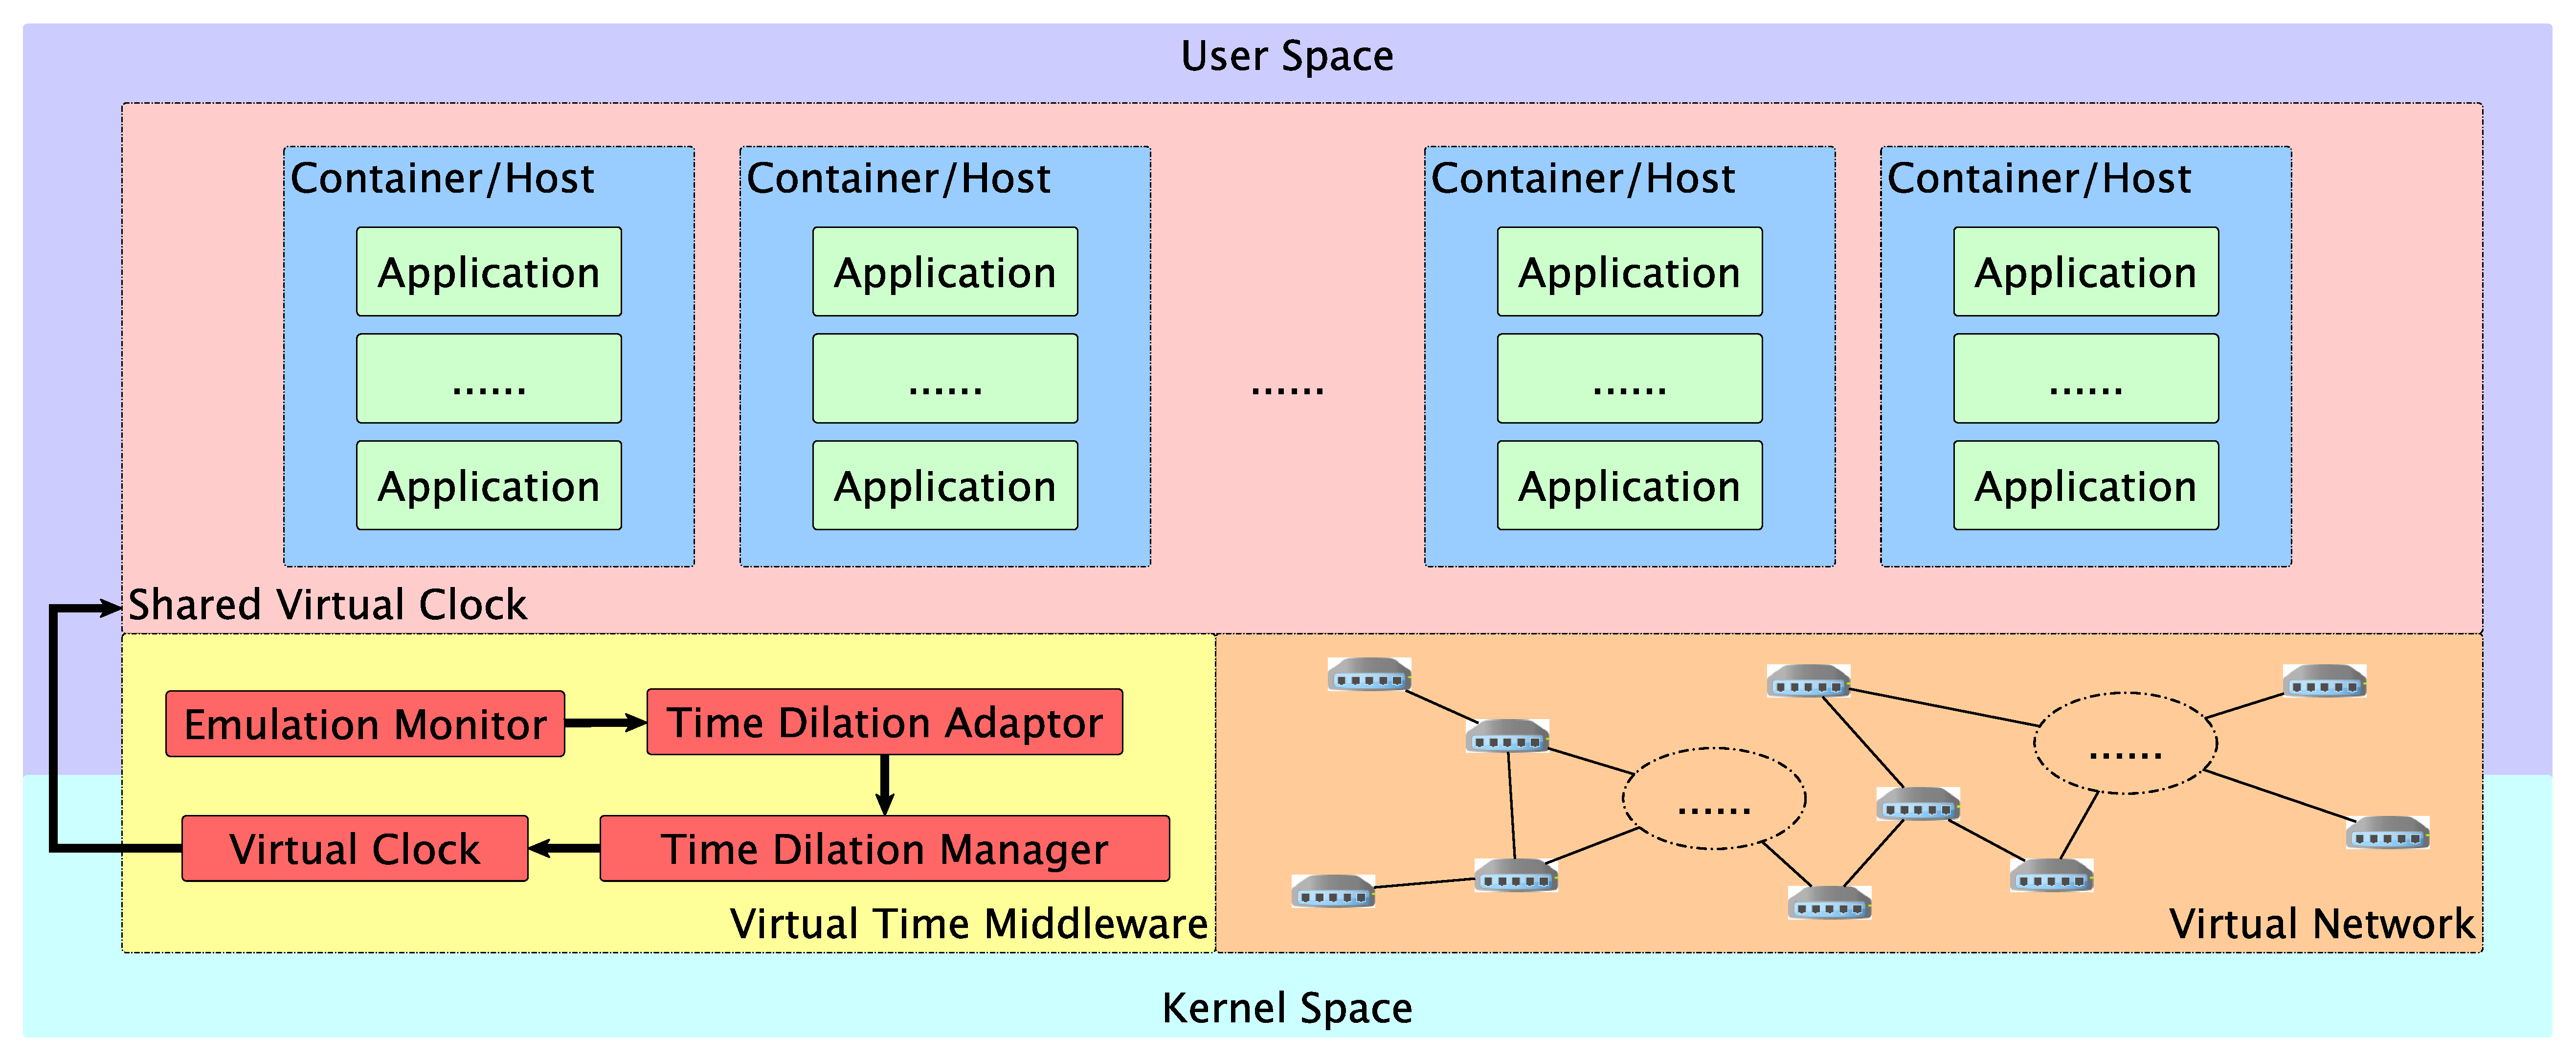
\epsfig{file=figures/ContainerVirtualTime.eps, height=2in, width=5in}
\caption{\textbf{Architecture of the Virtual Time System in a Container-based Network Emulator. Note that a typical container-based network emulator can be presented by this figure without the Virtual Time Middleware.}}
\label{Fig-ContainerVirtualTime}
\end{figure*}

\subsection{Virtual Time Management}
Our virtual time system, as shown in Figure \ref{Fig-ContainerVirtualTime}, is designed to meet all the requirements. The time dilation manager is responsible for computing and maintaining the virtual time, according to a given TDF for all the containers. It can offer per-container virtual time or the global virtual time for the emulator. The per-container virtual time is useful to support synchronized emulation (in virtual time) and facilitates the integration with network simulators. We have made a small set of changes in the kernel, in particular, a modified data structure to present virtual time, and a new algorithm to convert the elapsed wall-clock time to the dilated virtual time, with no dependency on third-party libraries.

We attach each container an integer-valued TDF, which could also be shared among all containers. A TDF of $k$ slows down a container's time advancement rate by a factor of $k$, thus re-scales a container's notion of time with reference to a physical network. This way, Mininet can emulate a seemingly $k$ times faster network owing to the accelerated rate of interaction between the containers and the virtual network
%When TDF is greater than 1, it appears to the containers that available resources including link bandwidth and CPU computation capacity are increased by a factor of TDF. 
Note that our design cannot scale the capacity of hardware components such as main memory, processor caches, and disk, firmware on network interfaces. 

The integration with Mininet, and potentially other container-based software is straightforward. We provide a set of simple APIs to (1) initialize containers with virtual time, and (2) inquire virtual time at run time. The system returns precise virtual time to container processes and transparently to all their child processes while returning the ordinary system time to other processes. We have integrated the system with Mininet. The implementation details are discussed in Section \ref{Sec-Implementation}, and we plan to make our code base available to public on GitHub soon. 

\subsection{Adaptive Time Dilation}

The key insight of virtual time is to trade time with available system resources. The execution time can be unnecessarily long with an overestimated TDF. It is difficult to avoid that with a fixed TDF when the resource demands vary substantially during the emulation. Therefore, we investigate means to adaptively adjust TDF in run-time with the goal of well balancing the execution speed and accuracy. We take a similar epoch-based approach described in \cite{NtwkEmultAdaptVirtTime}, and develop two modules, Emulation Monitor and Time Dilation Adaptor (see Figure \ref{Fig-ContainerVirtualTime}), to achieve the dynamic TDF adjustment. 

Emulation Monitor periodically collects the process-related information (not necessarily coincides with the epoch duration) and computes the run-time emulation load statistics, such as CPU utilization, number of waiting processes, or average process waiting time. Time Dilation Adaptor takes the inputs from Emulation Monitor, and adaptively computes the TDF for the next epoch based on a heuristic algorithm, whose details are presented in Section \ref{Sec-Implementation}. Currently we only use the CPU utilization as the feedback control indicator, and will leave the exploration of other control algorithms as future works. 

% Figure \ref{Fig-ContainerVirtualTime} presents the simplified structure of a regular container-based emulator if we eliminate all the parts inside the yellow rectangle. Usually, emulator will create container for each virtual host and later put the application that runs on a particular host into the correct container. As the key different from other virtualization techniques, container-based host share the guest OS's kernel; they are no different than a special process that think itself as the owner of the machine. In practice, it will be more efficient to put virtual network, including virtual switches, virtual interfaces and link, inside the kernel space. However, user space virtual network is also an option.

% Figure \ref{Fig-ContainerVirtualTime} also describes what the original architecture becomes after we add virtual time and dynamic time dilation management features in to the emulator. Since the only difference between with and without virtual time support is constrained inside the yellow part only, users can run previous experiments in no need of virtual time without any modification. To fulfill backward-compatibility, we add a middleware between (and inside) kernel and the containers application resides in. Such a design can let users execute applications or experiments that DOES need virtual time. If one wants to run his or her emulation with virtual time enabled, all one needs to do is to either feed a fixed time dilation factor or simply specify an dilation adaptor so that our system can take care of the dilation configuration from then on. In the term of software architecture, the network emulator with virtual time support can been seen as a 3-layered software: the Application Layer that includes containers and applications, the Virtual Time Management Middleware and OS Kernel Layer. We describe each layer one by one.

% \begin{figure*}
% \centering
% 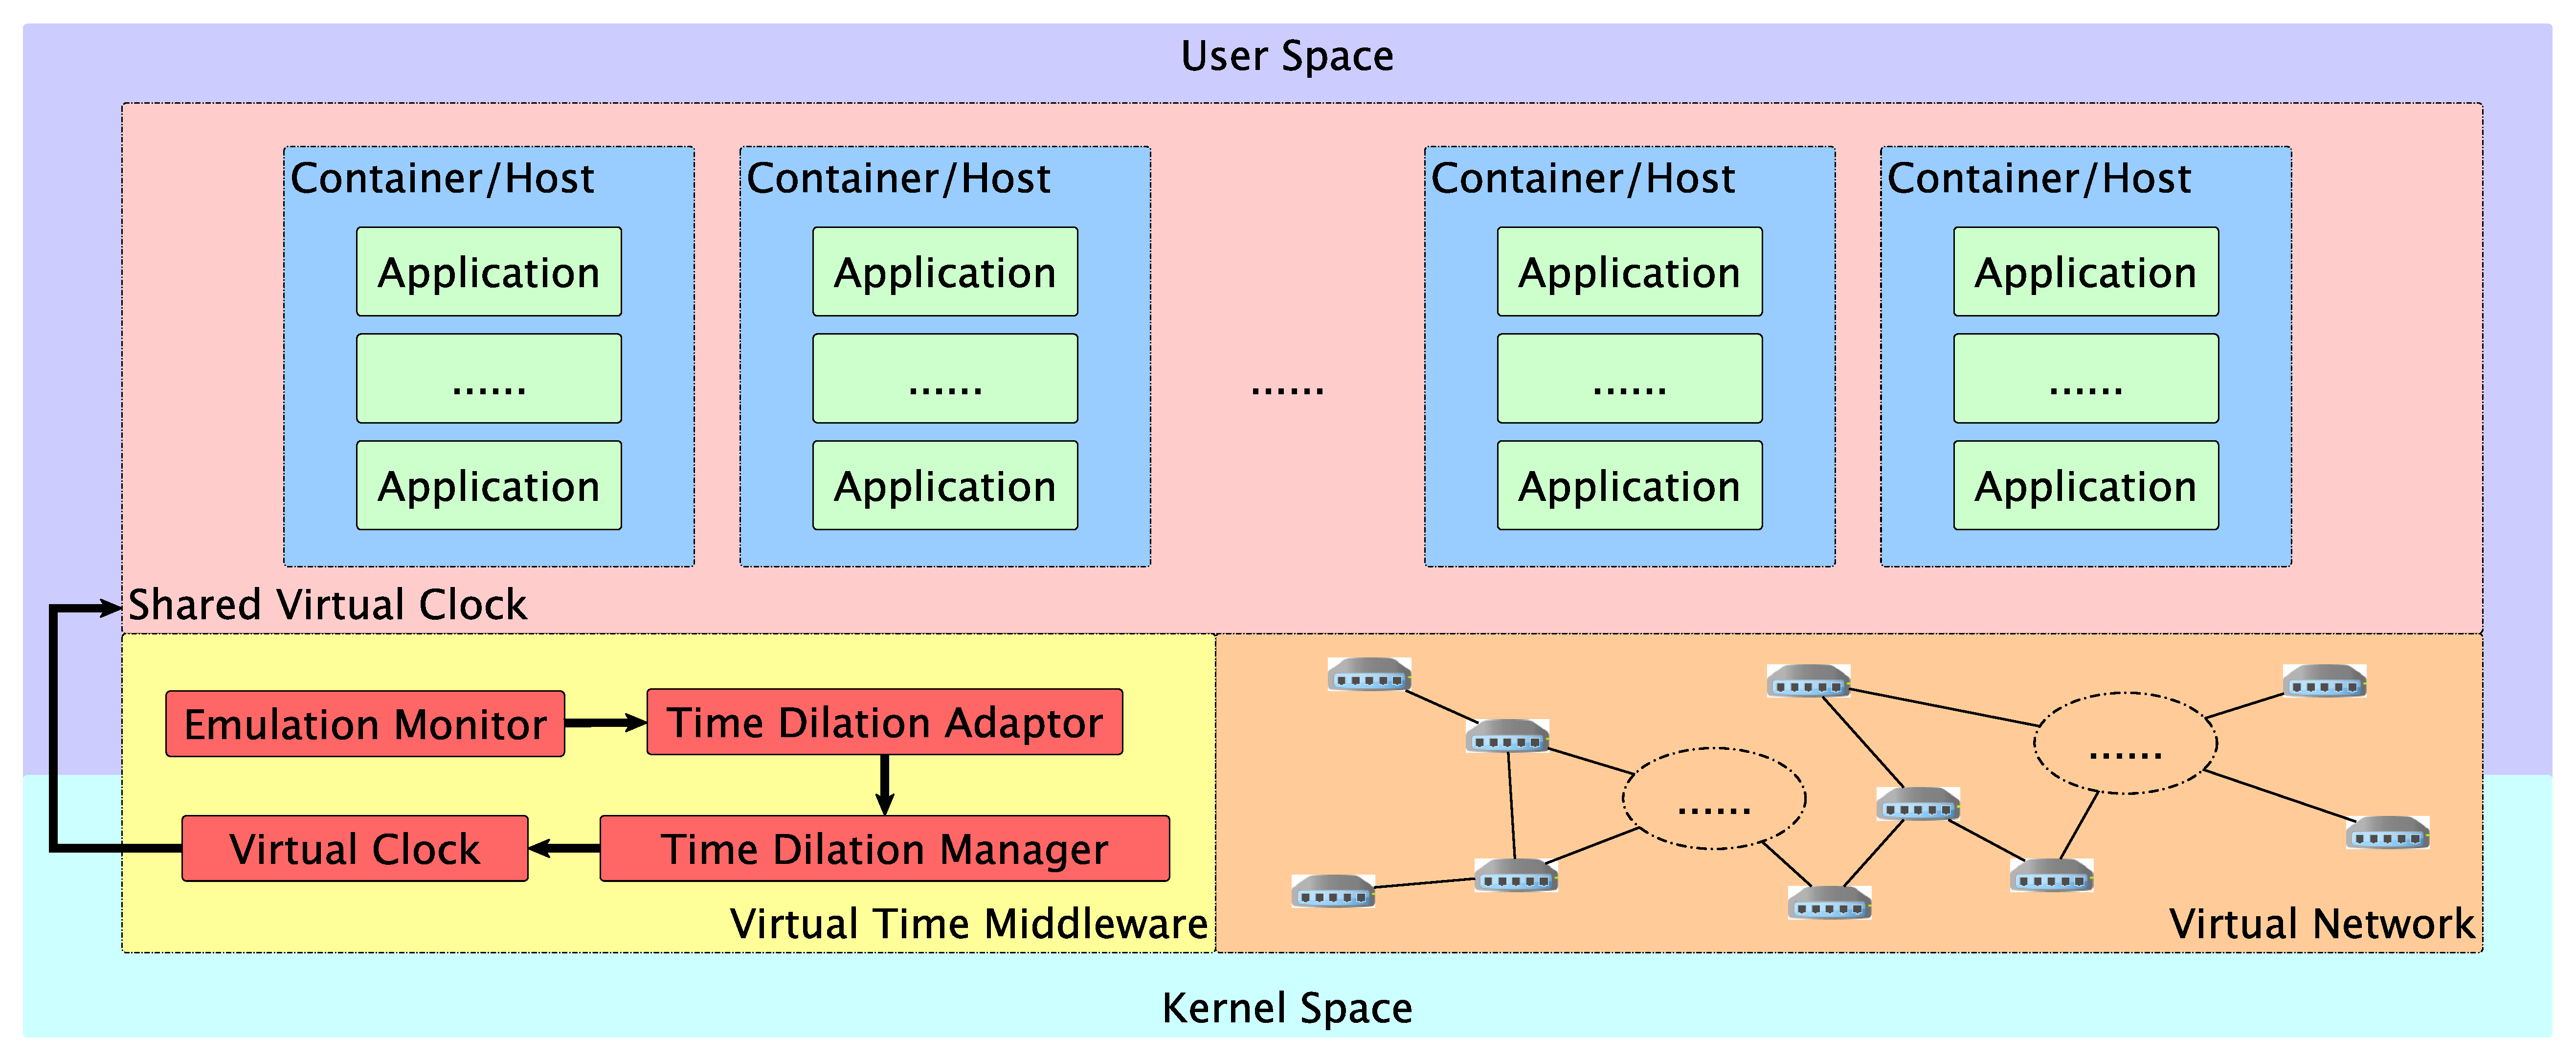
\epsfig{file=figures/ContainerVirtualTime.eps, height=2in, width=5in}
% \caption{\textbf{Virtual Time System Architecture Design with Integration of a Container-based Network Emulator}}
% \label{Fig-ContainerVirtualTime}
% \end{figure*}

% \subsection{OS Kernel Layer}
% In this layer, as shown in Figure \ref{Fig-ContainerVirtualTime}, we need to modify the kernel itself so that it has a virtual clock, e.g. the Virtual Time Supported Kernel. This involve patching many parts in the original kernel. For example, we should add data structures to present the virtual time, add algorithms to calculate virtual time from real time. Besides, in order to further schedule the speed of the Virtual Clock, a Time Dilation Management mechanism is a must. Those new features provided by modified kernel is available through new defined kernel APIs. Typically, we need to add an API to create a process that use virtual clock and an API to change a process's virtual clock speed. Returning virtual time to containers should use the old API that kernel uses when returning wall clock time. Only in this way can all the modifications be transparent to arbitrary applications.

% \subsection{Virtual Time Management Middleware}
% \label{Sub-Sec-VirtualTimeMiddleware}
% This layer exists as a service layer for applications that the users are interested to test with virtual time. If a user is willing to provide a time dilation because he or she already knows that the underlying hardware resource is not sufficient to run a experiment with high fidelity, emulator can accept it and enable virtual time right from the beginning of the emulation. Otherwise, our virtual time supported emulator is able to take care of the speed of the experiment for the users. That is to say, emulator have the freedom to choose a time dilation as large as possible such that experiment environment is scaled to the physical one that the user wants. However, it also have the responsibility to finish the experiment as soon as possible or report impossible to finish the experiment because it will take too long.

% In order to provide these features to user, our system borrows the concept of \textit{Epoch} from \cite{NtwkEmultAdaptVirtTime} to schedule time dilation factor. During an epoch, all virtual nodes in emulation run under the same constant TDF. Upon entering an new epoch, the emulator has the chance to tune the global TDF for itself. Epochs, naturally, should have distinguished characters of load, which measured by the system utilization, usually percentage of CPU time in practice.

% To collect load statistics of an Epoch and deal with the Epoch transition, we should have 2 modules in the virtual time management subsystem: Emulation Monitor and Time Dilation Adaptor. The Emulation Monitor polls OS periodically (may not coincides with Epoch's duration) and get comprehensive statistics that reflect the system load at run-time. In a container based network emulator, usually virtual nodes (including hosts, switches and controllers in a typical SDN network environment) are all processes inside independent containers; every application is being executed as child process of the node it runs on. Since containers are naturally separated from other processes in the same OS, it is quiet convenient to gather the load statistics only related to emulator. Using these information, emulator could consult Time Dilation Adaptor who returns an appropriate time dilation grounded on some heuristic algorithm. It can be as intuitive as the one in \cite{NtwkEmultAdaptVirtTime}. Note that changing TDF for a container actually happens in kernel space; emulator simply delegate this task to OS Kernel Layer who does the dirty works. 

% Our dynamic time dilation management system actually shares many concepts proposed by \cite{NtwkEmultAdaptVirtTime}, though the relation between Monitor and Adaptor in our design is different from theirs. However, the differences in implementation are significant. We will discuss these differences in subsection \ref{Sub-Sec-ImplementMininet}.

% \subsection{Application Layer}
% Emulator can directly create containers that virtualize network hosts. Each container has its own private network namespace/interface. After introducing virtual routing or virtual switch technique, a non-trivial network environment can be build upon a single machine. All containers are sharing the same virtual clock that can be faster or slower than the clock OS kernel uses. As for now, it only makes sense that all containers use virtual clocks of the same advance speed, e.g. share global time dilation factor. When using a time dilation factor (TDF) greater than 1, it appears to host that available resources, for example, link bandwidth and CPU computation capacity, increase to TDF times. However, as one of the most obvious and serious problem of virtual time, all the emulated hosts running TDF times slower now. Sometimes we can do nothing about it but notify user that the emulation have to take that long time because a smaller dilation cannot guarantee the target experiment environment. Fortunately, our Virtual Time Management Middleware can mitigate this problem in the cases that user feed an overestimated time dilation factor, or the resource demand varies during the emulation.

% Directly or indirectly, applications are developed on the basis of the APIs operating system exposed to the outside world. They are often kicked off by emulator. When adopting the design in Figure \ref{Fig-ContainerVirtualTime}, we do not need to modify anything in the applications; applications still ask for anything they need through the same API from software library or OS kernel, for example, asking for time. 

\section{Implementation}
\label{Sec-Implementation}

The implementation of the virtual time system and its integration with Mininet-Hifi (the latest version of Mininet) is composed of three parts, as shown in Figure \ref{Fig-VT-Mininet-Hifi}. First, we built a lightweight and independent middleware in the Linux kernel to provide virtual time support to user-space software. Second, we slightly modified the initialization procedure of Mininet with two additional python modules to realize (adaptive) virtual time in Mininet. Third, we discuss our design to enable transparent support of virtual time for applications running in the containers.

\begin{figure*}
\centering
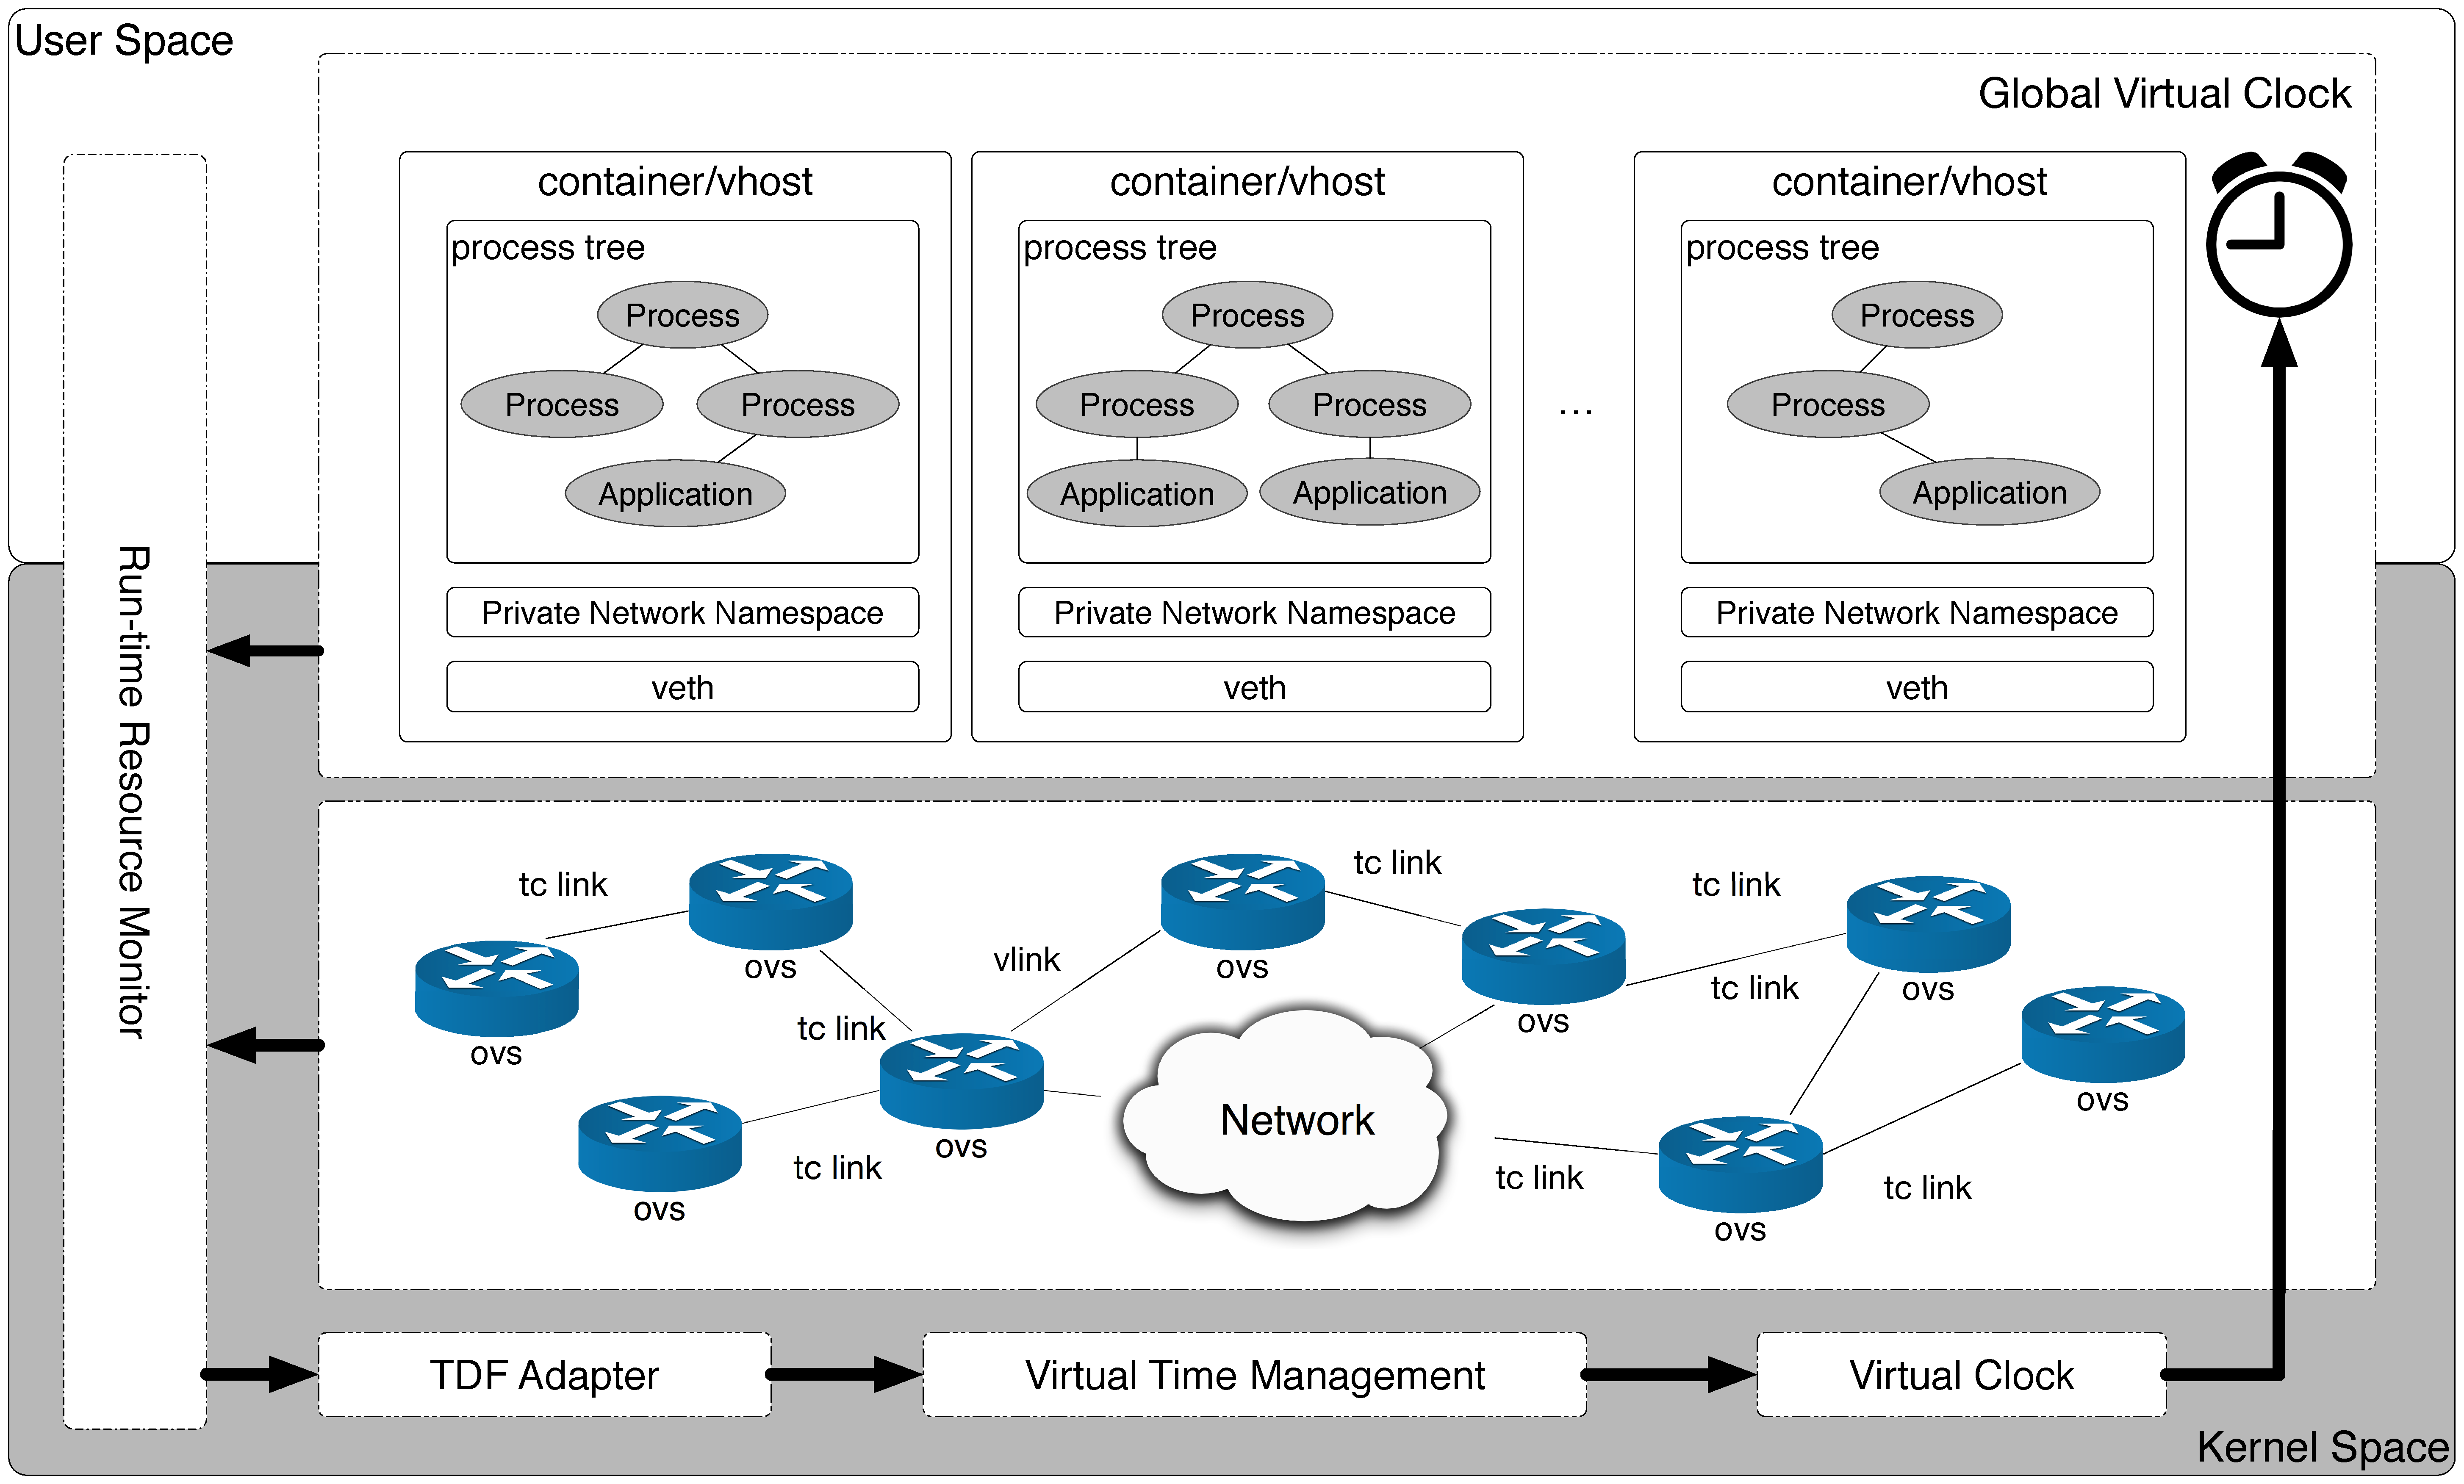
\epsfig{file=figures/VT-Mininet-Hifi.eps, height=3.3in, width=5.5in}
\caption{\textbf{Integration of Mininet-Hifi and Virtual Time}}
\label{Fig-VT-Mininet-Hifi}
\end{figure*}

\subsection{Linux Kernel Modifications}
\label{Sub-Sec-ExtendLinuxKernel}

Our implementation is based on a recent Linux kernel 3.16.3 with no third-part library dependency.

\subsubsection{Timing-related Kernel Modifications}
To make a process have its own perception of time, we added the following four new fields in the \texttt{task\_struct} struct type.
\begin{itemize}
	\item \texttt{virtual\_start\_nsec} represents the starting time that a process detaches from the system clock and uses the virtual time, in nanoseconds 
	\item \texttt{physical\_past\_nsec} represents how much physical time has elapsed since the last time the process requested the current time, in nanoseconds 
	\item \texttt{virtual\_past\_nsec} represents how much virtual time has elapsed since the last time the process requested the current time, in nanoseconds
	\item \texttt{dilation} represents the TDF of a time-dilated process
\end{itemize}

\setlength{\textfloatsep}{0pt}% Remove \textfloatsep
\setlength{\intextsep}{0pt}
\setlength{\floatsep}{0pt}
\algrenewcommand{\algorithmiccomment}[1]{\hskip3em$/*$ #1 $*/$}
\begin{algorithm*}[t]
\caption{Time Dilation Algorithm}%: Dilate \texttt{ts} if a current process uses virtual clock}
\label{Alg-DilateTimeKeeping}
\begin{algorithmic}[1]
\Function{init\_virtual\_time}{\texttt{struct task\_struct *tk, int dilation}}
\If{\texttt{dilation>0}}
    \State \texttt{tk$\rightarrow$virtual\_start\_nsec=0}
    \State \texttt{struct timespec ts}
    \State \texttt{getnstimeofday(\&ts)}
    \State \texttt{tk$\rightarrow$virtual\_start\_nsec=timespec\_to\_ns(\&ts)}
    \State \texttt{tk$\rightarrow$physical\_past\_nsec=0}
    \State \texttt{tk$\rightarrow$virtual\_past\_nsec=0}
    \State \texttt{tk$\rightarrow$dilation=dilation}
\EndIf
\EndFunction
\\
\Function{do\_dilatetimeofday}{\texttt{struct timespec *ts}}
\State{Let \texttt{p} denote the current process using virtual time} %system-wide}
\If{\texttt{p$\rightarrow$virtual\_start\_nsec > 0  and p$\rightarrow$dilation > 0}}
	\State \texttt{now = timespec\_to\_ns(ts)}
	\State \texttt{physical\_past\_nsec = now - p$\rightarrow$virtual\_start\_nsec}
	\State \texttt{virtual\_past\_nsec = (physical\_past\_nsec - p$\rightarrow$physical\_past\_nsec) / p$\rightarrow$dilation + p$\rightarrow$virtual\_past\_nsec}\Comment{virtual time computation}
	\State \texttt{dilated\_now = virtual\_past\_nsec + p$\rightarrow$virtual\_start\_nsec}
	\State \texttt{dilated\_ts = ns\_to\_timespec(dilated\_now)}
	\State \texttt{ts$\rightarrow$tv\_sec = dilated\_ts.tv\_sec}
	\State \texttt{ts$\rightarrow$tv\_nsec = dilated\_ts.tv\_nsec}
	\State \texttt{p$\rightarrow$physical\_past\_nsec = physical\_past\_nsec}\Comment{update process's physical time}
	\State \texttt{p$\rightarrow$virtual\_past\_nsec = virtual\_past\_nsec}\Comment{update process's virtual time}
\EndIf
\EndFunction
\end{algorithmic}
\end{algorithm*}
Algorithm \ref{Alg-DilateTimeKeeping} gives the details about how we implement the time dilation. 
To preserve an accurate virtual clock in the kernel, we added a private function \texttt{do\_dilatetimeofday} in the Linux's timekeeping subsystem to keep tracking the dilated virtual time based on the physical time passed and TDF. 
Based on process's \texttt{virtual\_start\_nsec}, the system determines the type of time to return, i.e., the physical system clock time or the virtual time.

\texttt{virtual\_start\_nsec} in \texttt{INIT\_VIRTUAL\_TIME} should first be initialized to zero so that the next gettimeofday always returns the undilated time to compute and record the exact physical time that a process starts to use virtual time.
To return the accurate virtual time upon requests, the duration since the last call to \texttt{do\_dilatetimeofday} is calculated and precisely scaled with TDF. 
To enable virtual time support for a wide range of timing-related system calls, we extensively traced the routines in Linux's subsystems that request timing information (such as \texttt{getnstimeofday}, \texttt{ktime\_get}, \texttt{ktime\_get\_ts}, etc.), and modified them to properly invoke \texttt{do\_dilatetimeofday}.


\subsubsection{Process-related Kernel Modifications}
To enable the virtual time perception to processes running in a network emulator, we added the following new system calls.
\begin{itemize}
\item \texttt{virtualtimeunshare} is essentially the \texttt{unshare} system call with time dilation inputs. It is used by container-based emulators, such as Mininet, to create emulated nodes. \texttt{virtualtimeunshare} creates a new process with a TDF in a different \texttt{namespace} of its parent process according to \texttt{flags}.
\item \texttt{settimedilaitonfactor} offers an interface to change the TDF of a process. Note that a command executed in an emulated host is equivalent to forking a shell command executed by \texttt{bash}. 
Therefore, adjusting a process' TDF requires the change of the calling process' parent (e.g., host's \texttt{bash}), which occasionally would lead to tracing back to the root of the process tree, especially in the case of dynamic TDF adjustment. 
\end{itemize}

We also modified the \texttt{do\_fork} system call to initialize the virtual-time-related attributes of a process, such as using the variable \texttt{stack\_size} to pass the TDF value. 
Another option is to set TDF to a default value in \texttt{virtualtimeunshare} and then relies on explicitly invoking \texttt{settimedilationfactor} to set desired TDF; this method prevents modifying the interface of creating \texttt{namespace} in traditional Linux. 
Functions in \texttt{timekeeping.c} were modified to invoke \texttt{do\_dilatetimeofday} in order to return the virtual time to system calls like \texttt{gettimeofday} and other kernel routines that request timing information.


\subsubsection{Networking-related Kernel Modifications}
In this work, we focus on capturing all the related system calls and kernel routings to support virtual time in Linux container with the application of Mininet. 
One particular case related to Mininet is the usage of \texttt{tc}, a network quality-of-service control module in Linux\cite{TrafficControl}. 
For instance, we can use \texttt{tc} to rate-limit a link to 100 Mbps using Hierarchic Token Bucket (HTB) \texttt{qdisc} in Mininet. If the TDF is set to 8, the link bandwidth would be approximately 800 Mbps from the emulated hosts' viewpoints as we observed from the time-dilated \texttt{iperf3} application.

As a network module in Linux, \texttt{tc} does not reference Linux kernel's time as the way user application does. 
Therefore, \texttt{tc} is transparent to our virtual time system. One way to solve this problem is to modify the network scheduling code in kernel to provide \texttt{tc} with a dilated traffic rate. 
In the earlier example with TDF set to 8, the experiment will run 8 times slower than the real time, and we can configure \texttt{tc}'s rate limit as $rate/TDF=12.5$ Mbps to emulate a 100 Mbps link. 
Note that we only tailored HTB in \texttt{tc}, which is the default \texttt{qdisc} used by Mininet. 
We will generalize the mechanism to other \texttt{qdiscs} including HFSC (Hierarchical Fair Service Curve) and TBF (Token Bucket Filter) in the future.

\subsection{Network Emulator Modifications}
\label{Sub-Sec-ImplementMininet}

\subsubsection{Virtual-Time-Enabled Container}
%Mininet uses Linux's container \cite{LXC} to enable scalable network emulation. 
Containers allow groups of process running on the same kernel to have independent views of system resources, such as process IDs, file systems and network interfaces. 
We add the virtual time property to a container's \texttt{namespace}\cite{LinuxNamespace} so that every container can have its own virtual clock. 
We design our system in the way that minimal modifications of Mininet are needed for integration, so that the virtual time system can be easily extended to other Linux-container-based applications. 

We modified the initialization procedure of Mininet, in particular, the \texttt{mnexec} program in Mininet, to process two additional parameters. 
When we create \texttt{Node}s in Mininet (hosts, switches, and controllers are all inherited from \texttt{Node}), users can feed in a TDF argument with \texttt{virtualtimeunshare} (as a replacement of \texttt{unshare}) with \texttt{-n} option. 
This way, a system-wide TDF can be conveniently set for all the emulated hosts. We also provide the ability to dynamically adjust the TDF for every emulated host during runtime. 
To do that, we added a new option \texttt{-t} in \texttt{mnexec} to invoke the aforementioned system call \texttt{settimedilaitonfactor} to do the actual TDF adjustment. 
The two modifications enable the integration of virtual time in Mininet, and also serve as the basis of the adaptive TDF management.

\subsubsection{Adaptive TDF Scheduling}
To optimize the performance of the virtual-time-enabled Mininet, we developed an adaptive TDF scheduler through two python modules \texttt{MininetMonitor} and \texttt{DilationAdaptor} (refer to Emulation Monitor and Time Dilation Adaptor in Figure \ref{Fig-ContainerVirtualTime}) to accelerate the experiment speed while preserving high fidelity.

\texttt{MininetMonitor} is responsible to monitor the CPU usage of the entire emulation system, consisting of a group of processes including the Mininet emulator, the Open vSwitch module, and emulated nodes (e.g., SDN controllers, hosts and switches). 
Also, applications are dynamically created, executed and destroyed within containers, in the form of child processes of their parent containers. 
\texttt{MininetMonitor} utilizes the \texttt{ps} command to collect the group's aggregate CPU percentage and periodically computes and passes the average CPU load statistics to \texttt{DilationAdaptor}. 
The core of \texttt{DilationAdaptor} is an adaptive algorithm to calculate an appropriate \textit{TDF}. %Only after receiving a new \textit{TDF} can Mininet pause the experiment and update its global time dilation factor. Otherwise it enters the next Epoch directly. 
Global \textit{TDF} updating was achieved by invoking the \texttt{mnexec\ -t\ tdf} program for every running host. 


% Algorithm \ref{Alg-AdaptiveTDF} illustrates our adaptive TDF scheduling, and we implemented it as a threshold-based \texttt{DilationAdaptor}. 
% %From the input fed by \texttt{MininetMonitor}, \texttt{DilationAdaptor} first define current load status. The key idea here is: if emulator is overloaded, we increase TDF with a large value; if it is underloaded, we may consider decrease TDF with a large value. 

% \algnewcommand\algorithmicswitch{\textbf{switch}}
% \algnewcommand\algorithmiccase{\textbf{case}}
% \algnewcommand\algorithmicassert{\texttt{assert}}
% \algnewcommand\Assert[1]{\State \algorithmicassert(#1)}%
% % New "environments"
% \algdef{SE}[SWITCH]{Switch}{EndSwitch}[1]{\algorithmicswitch\ #1\ \algorithmicdo}{\algorithmicend\ \algorithmicswitch}%
% \algdef{SE}[CASE]{Case}{EndCase}[1]{\algorithmiccase\ #1}{\algorithmicend\ \algorithmiccase}%
% \algtext*{EndSwitch}%
% \algtext*{EndCase}%

% \algrenewcommand{\algorithmiccomment}[1]{\hskip1em$/*$ #1 $*/$}
% \begin{algorithm}
% \caption{Adaptive Time Dilation Factor Scheduling}\label{Alg-AdaptiveTDF}
% \begin{algorithmic}[1]
% \State{Decide emulation $state$ through the resource indicator}\Comment{e.g., CPU utilization}
% \State{$MAX$ denotes the maximum allowed TDF value.}
% \State{$\Delta_{large}, \Delta_{small}$ denote the customizable large and small adjustment}
% \Switch{$state$}
% 	\Case{$OVERLOADED$}
% 		\State{$TDF_{new}=TDF_{prev}+\Delta_{large}$}
% 	\EndCase
% 	\Case{$WARNING$}
% 		\State{$TDF_{new}=TDF_{prev}+\Delta_{small}*2$}
% 	\EndCase
% 	\Case{$MODERATE$}
% 		\If{$TDF_{prev} == MAX$}
% 			\State{$TDF_{new}=TDF_{prev}-\Delta_{large}$}
% 		\ElsIf{$TDF_{prev} > \Delta_{small}$}
% 			\State{$TDF_{new}=TDF_{prev}-\Delta_{small}$}
% 		\Else
% 			\State{$TDF_{new}=TDF_{prev}$}%\Comment{Do not change TDF}
% 		\EndIf
% 	\EndCase
% 	\Case{$LIGHT$}
% 		\If{$TDF_{prev} > \Delta_{large}*2$}
% 			\State{$TDF_{new}=TDF_{prev}-\Delta_{large}$}
% 		\Else
% 			\State{$TDF_{new}=TDF_{prev}-\Delta_{small}*2$}
% 		\EndIf
% 	\EndCase
% \EndSwitch
% %\State{return $TDF_{new}$}
% \end{algorithmic}
% \end{algorithm}

Our adaptive virtual time scheduling design is similar to the one used in \cite{NtwkEmultAdaptVirtTime} in spirit with two major differences. 
First, both techniques target on different platforms. 
Our technique is applied to Linux-container-based network emulation to support scalable SDN experiments, and theirs uses virtual routing and executes OpenVZ instances inside Xen. 
Second, their solution needs be deployed on a cluster to emulate a medium-scale network, which results in much higher communication overhead in two types: (1) every VM's monitor needs to report the CPU usage, and (2) the adaptor needs to send new TDF to every VM. 
Therefore, the message transmission delay in LAN and the processing delay in protocol stacks contributes to the overall communication delay. 
In contrast, \texttt{MininetMonitor} runs as a lightweight background thread in Mininet, and \texttt{DilationAdaptor} is simply a python object that Mininet has a reference to. 
The communication in our system is through synchronized queues and method invocations, which is much faster. 

\subsection{Virtual Time Support for Applications in Containers}
\label{Sub-Sec-ModificationApplications}
Network applications running inside containers (e.g., \texttt{iperf3}\cite{iperf3} or \texttt{ping}) should also use virtual time. 
We do not need to modify the application code because they are running as child processes of Mininet's hosts. 
A child process always copies its parent's \texttt{task\_struct} when it is forked including the same \texttt{dilation} and \texttt{virtual\_start\_nsec} values. 
Although \texttt{virtual\_start\_nsec} does not present the virtual starting time of the child process, our algorithm is designed to work with relative values since it does necessary initial processes during \texttt{do\_fork}. 
When applications inquire about the system time, the modified kernel knows that they are using virtual clock and return the virtual clock time instead of the system clock time.

One issue we notice is that the 64-bit Linux kernel running on Intel-based architectures provides the Virtual Dynamic Shared Object (vDSO) and the \texttt{vsyscall} mechanism to reduce the overhead of context switches caused by the frequently invoked system calls, for example, \texttt{gettimeofday} and \texttt{time}\cite{VDSO}. 
Therefore, applications may bypass our virtual-time-based system calls unless we explicitly use the \texttt{syscall} function. Our solution is to disable vDSO with respect to \texttt{\_\_vdso\_gettimeofday} in order to transparently offer virtual time to applications in the containers.

\section{Evaluation}
\label{Sec-Experiments}

In this section, we give experimental results to validate our implementation of the virtual time supported Mininet-Hifi network emulator. Very straightforward but nontrivial network typologies are adopted to demonstrate that the emulation system described in \ref{Sec-Implementation} can improve fidelity, scalability as well as efficiency. 

All the experiments are conducted on a Dell XPS 8700 Desktop with one Intel Core i7-4790 CPU, 12 GB RAM and one gigabit Ethernet interface. The machine runs a 64-bit Ubuntu 14.04.1 LTS with our customized 3.16.3 Linux kernel. The benchmark scores of this machine's CPU and FPU are: 1.52 seconds for Blowfish, 1045.62 MiB/seconds for CryptoHash, 0.63 seconds for FFT and 2.56 seconds for Raytracing. Our virtual-time-enabled Mininet was built on the latest version of Mininet (2.1.0), also named Mininet-Hifi, at the time of development.

\paragraphb{Fidelity.}
We first evaluate how our virtual time system improves Mininet's fidelity through a basic network scenario:  a single TCP flow transmission through a chain of switches in an emulated SDN network. As shown in Figure \ref{Fig-ChainTopoExample}, the network topology consists of a client-server pair connected by a chain of Open vSwitch switches in Mininet. We setup the default OpenFlow controller to function as a learning switch. In this set of experiments, we connected two hosts through 40 switches in Mininet, and all the links are configured with 10 $\mu s$ delay. We used \texttt{iperf3}\cite{iperf3} to generate a TCP flow between the client and the server. TDF was set to 1 (i.e., no virtual time) and 4 for comparison. We also setup a real testbed for ``ground truth" throughput data collection. The testbed was composed of two machines connected by a 10 Gbps Ethernet link. We varied the bandwidth link from 100 Mbps to 10 Gbps and measured the throughput using \texttt{iperf3}. In the real testbed, we manually configured the link bandwidth and delay using \texttt{tc}, and the delay was set as the corresponding round trip times (RTTs) measured in the switch chain topology in Mininet, so that the networking settings were tightly coupled for comparison. Although we did not setup an exact network with SDN switches, the stabilized TCP throughputs generated by the physical testbed should reflect what occurs in a real SDN network. Each experiment was repeated 10 times and the results with bandwidth 4 Gbps, 8 Gbps and 10 Gbps were reported in Figure \ref{Fig-Perf40SwDiffBw}. 


We observe that when the bandwidth was no greater than 4 Gbps (we only displayed the 4 Gbps case in the figure),  Mininet was able to accurately emulate the TCP flow with and without virtual time, as the average throughputs were very close to the ones collected from the physical testbed. However, when we continued to increase the bandwidth, Mininet was not able to produce the desired throughputs, e.g., 28\% (8 Gbps) and 39\% (10 Gbps) smaller than the physical testbed throughputs. With virtual time (TDF = 4), Mininet was capable to accurately emulate the TCP flow even at high bandwidth, and the results were nearly the same as the ones measured in the physical testbed. 

The root cause is that the machine running Mininet does not have sufficient resources to emulate networks with bandwidth greater than 4 Gbps, which would lead to fidelity issues, e.g., low expected throughputs.
% and higher throughput in the 8 Gbps case than the 10 Gbps case. By examining the TCP flows, we observed that in the 10 Gbps case, the congestion window (cwnd) never reached 4 MB because of multiple re-transmissions (around 450 times in 1 seconds) caused by packet losses and long latency, whereas in the 8 Gbps case, cwnd could reach 6.75 MB. 
Note that we only emulated a single flow, and the results could be much worse and unpredictable in complicated multi-flow scenarios. Results show that virtual time can significantly enhance the performance fidelity by ``slowing down" the experiments so that the system has sufficient resources and time to correctly process the packets. We further illustrate the effect by plotting the time series of throughput changes for the 10 Gbps cases in Figure \ref{Fig-Perf40Sw10GbLink}. With virtual time, the throughputs measured in Mininet closely match the real testbed results; without virtual time ($TDF = 1$), the ramp up speed was much slower, in particular, 22 seconds ($TDF = 1$) rather than 4 seconds ($TDF = 4$), and the throughput was incorrectly stabilized below 6.1 Gbps.

\paragraphb{Scalability.}
Virtual time also improves the scale of networks that one can emulate without losing fidelity. In this set of experiments, we used the same switch chain topology in Figure \ref{Fig-ChainTopoExample}, and set the link bandwidth to 4 Gbps. We want to investigate, with virtual time, how many switches Mininet is capable to emulate without losing fidelity, i.e., preserving nearly 4 Gbps throughput. This time we increased the number of switches with the following values \texttt{\{20, 40, 60, 80, 100\}}, and TDF was selected to be 1 (no virtual time) and 4. We ran \texttt{iperf3} for 25 seconds between the client and the server. Each experiment was repeated ten times, and the throughput measurement is reported in Figure \ref{Fig-ScaleDiffSw4GbLink}.

In the case of $TDF = 1$, the average throughput kept decreasing as the number of switches grew over 20. The throughput decreased dramatically when the number of switches was greater than 60 (e.g., decreased by 41\% for 60 switches, 65\% for 80 switches, and 83\% for 100 switches). The standard deviation, indicated the undesired high disturbance, also grew as number of switches increased. When virtual time was applied with $TDF = 4$, the throughput was always around 3.8 Gbps with small standard derivations in all the experiments. It is clear that virtual time helps to scale up the emulation. In this case, Mininet can emulate 100 switches with 4 Gbps links and still generate the accurate throughputs, rather than being saturated at 20 switches without virtual time. 

We also recorded the running time in Figure \ref{Fig-ScaleTime}. Longer execution time is the tradeoff for the fidelity and scalability improvement. When $TDF=4$, the execution time was about 4 times longer than the time required in the case of $TDF=1$ in all the experiments. In fact, we have conducted extensive experiments with different TDF values on multiple network scenarios. The general observation is that a larger TDF allows an emulator to conduct accurate experiments with larger scale on the same physical machine, but typically requires longer execution time, approximately proportional to the TDF.  This leads to the question on how to balance the speed and fidelity, and our approach is to explore the adaptive time dilation scheduling, whose evaluation is presented in the next section. 

\begin{figure*}
\centering
	\subfloat[\textbf{Switch Chain Topology for Fidelity and Scalability Evaluation}]
	{
		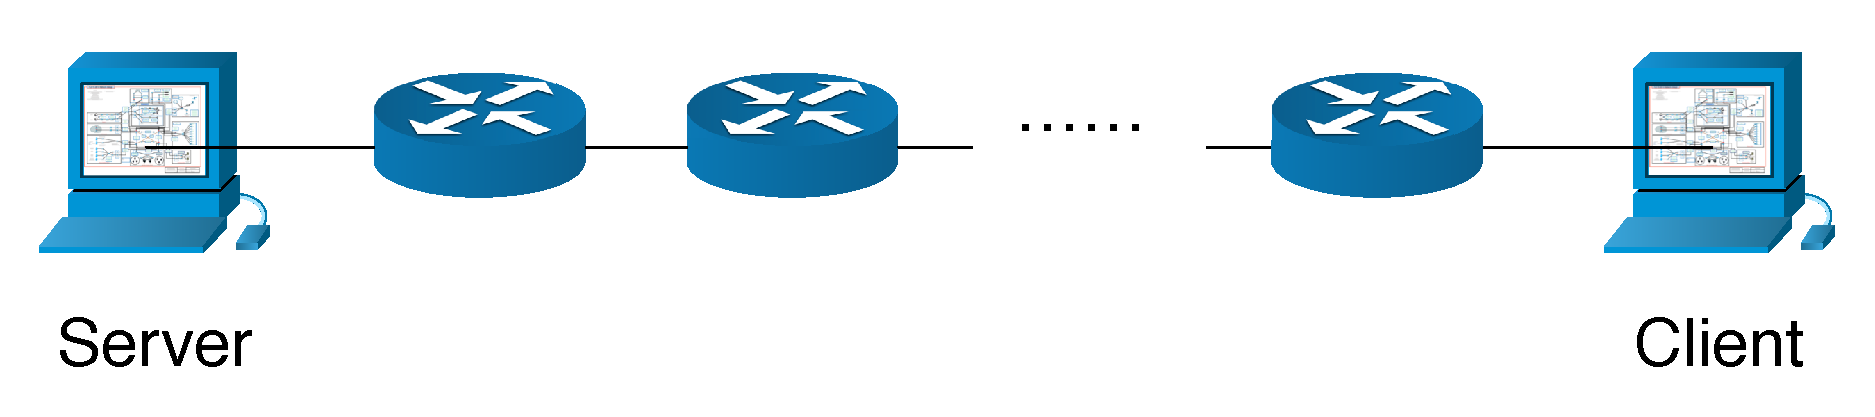
\epsfig{file=figures/TopoChainExample.eps, height=0.5in, width=2.6in}
		\label{Fig-ChainTopoExample}
	}~
	\subfloat[\textbf{Network Topology for Adaptive Virtual Time Evaluation}]
	{
		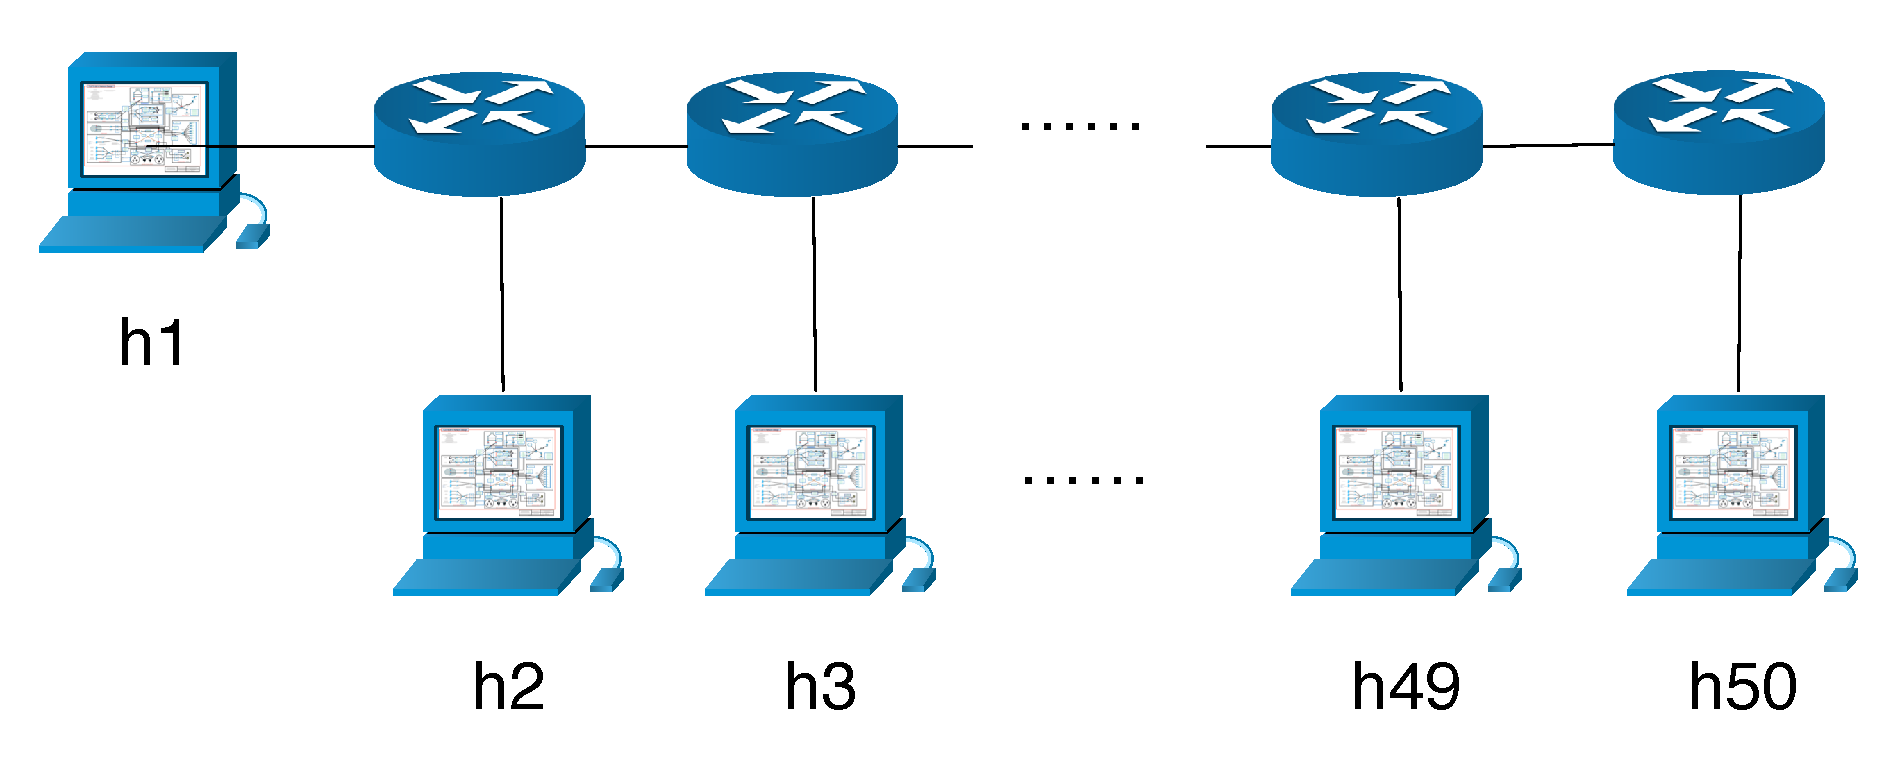
\epsfig{file=figures/TopoLinearExample.eps, height=1.0in, width=2.7in}
		\label{Fig-LinearTopoExample}
	}
	\caption{\textbf{Network Topologies for Evaluation}}
\end{figure*}

\begin{figure*}
\centering
	\subfloat[\textbf{TCP Throughput with Different Link Bandwidth}]
	{
		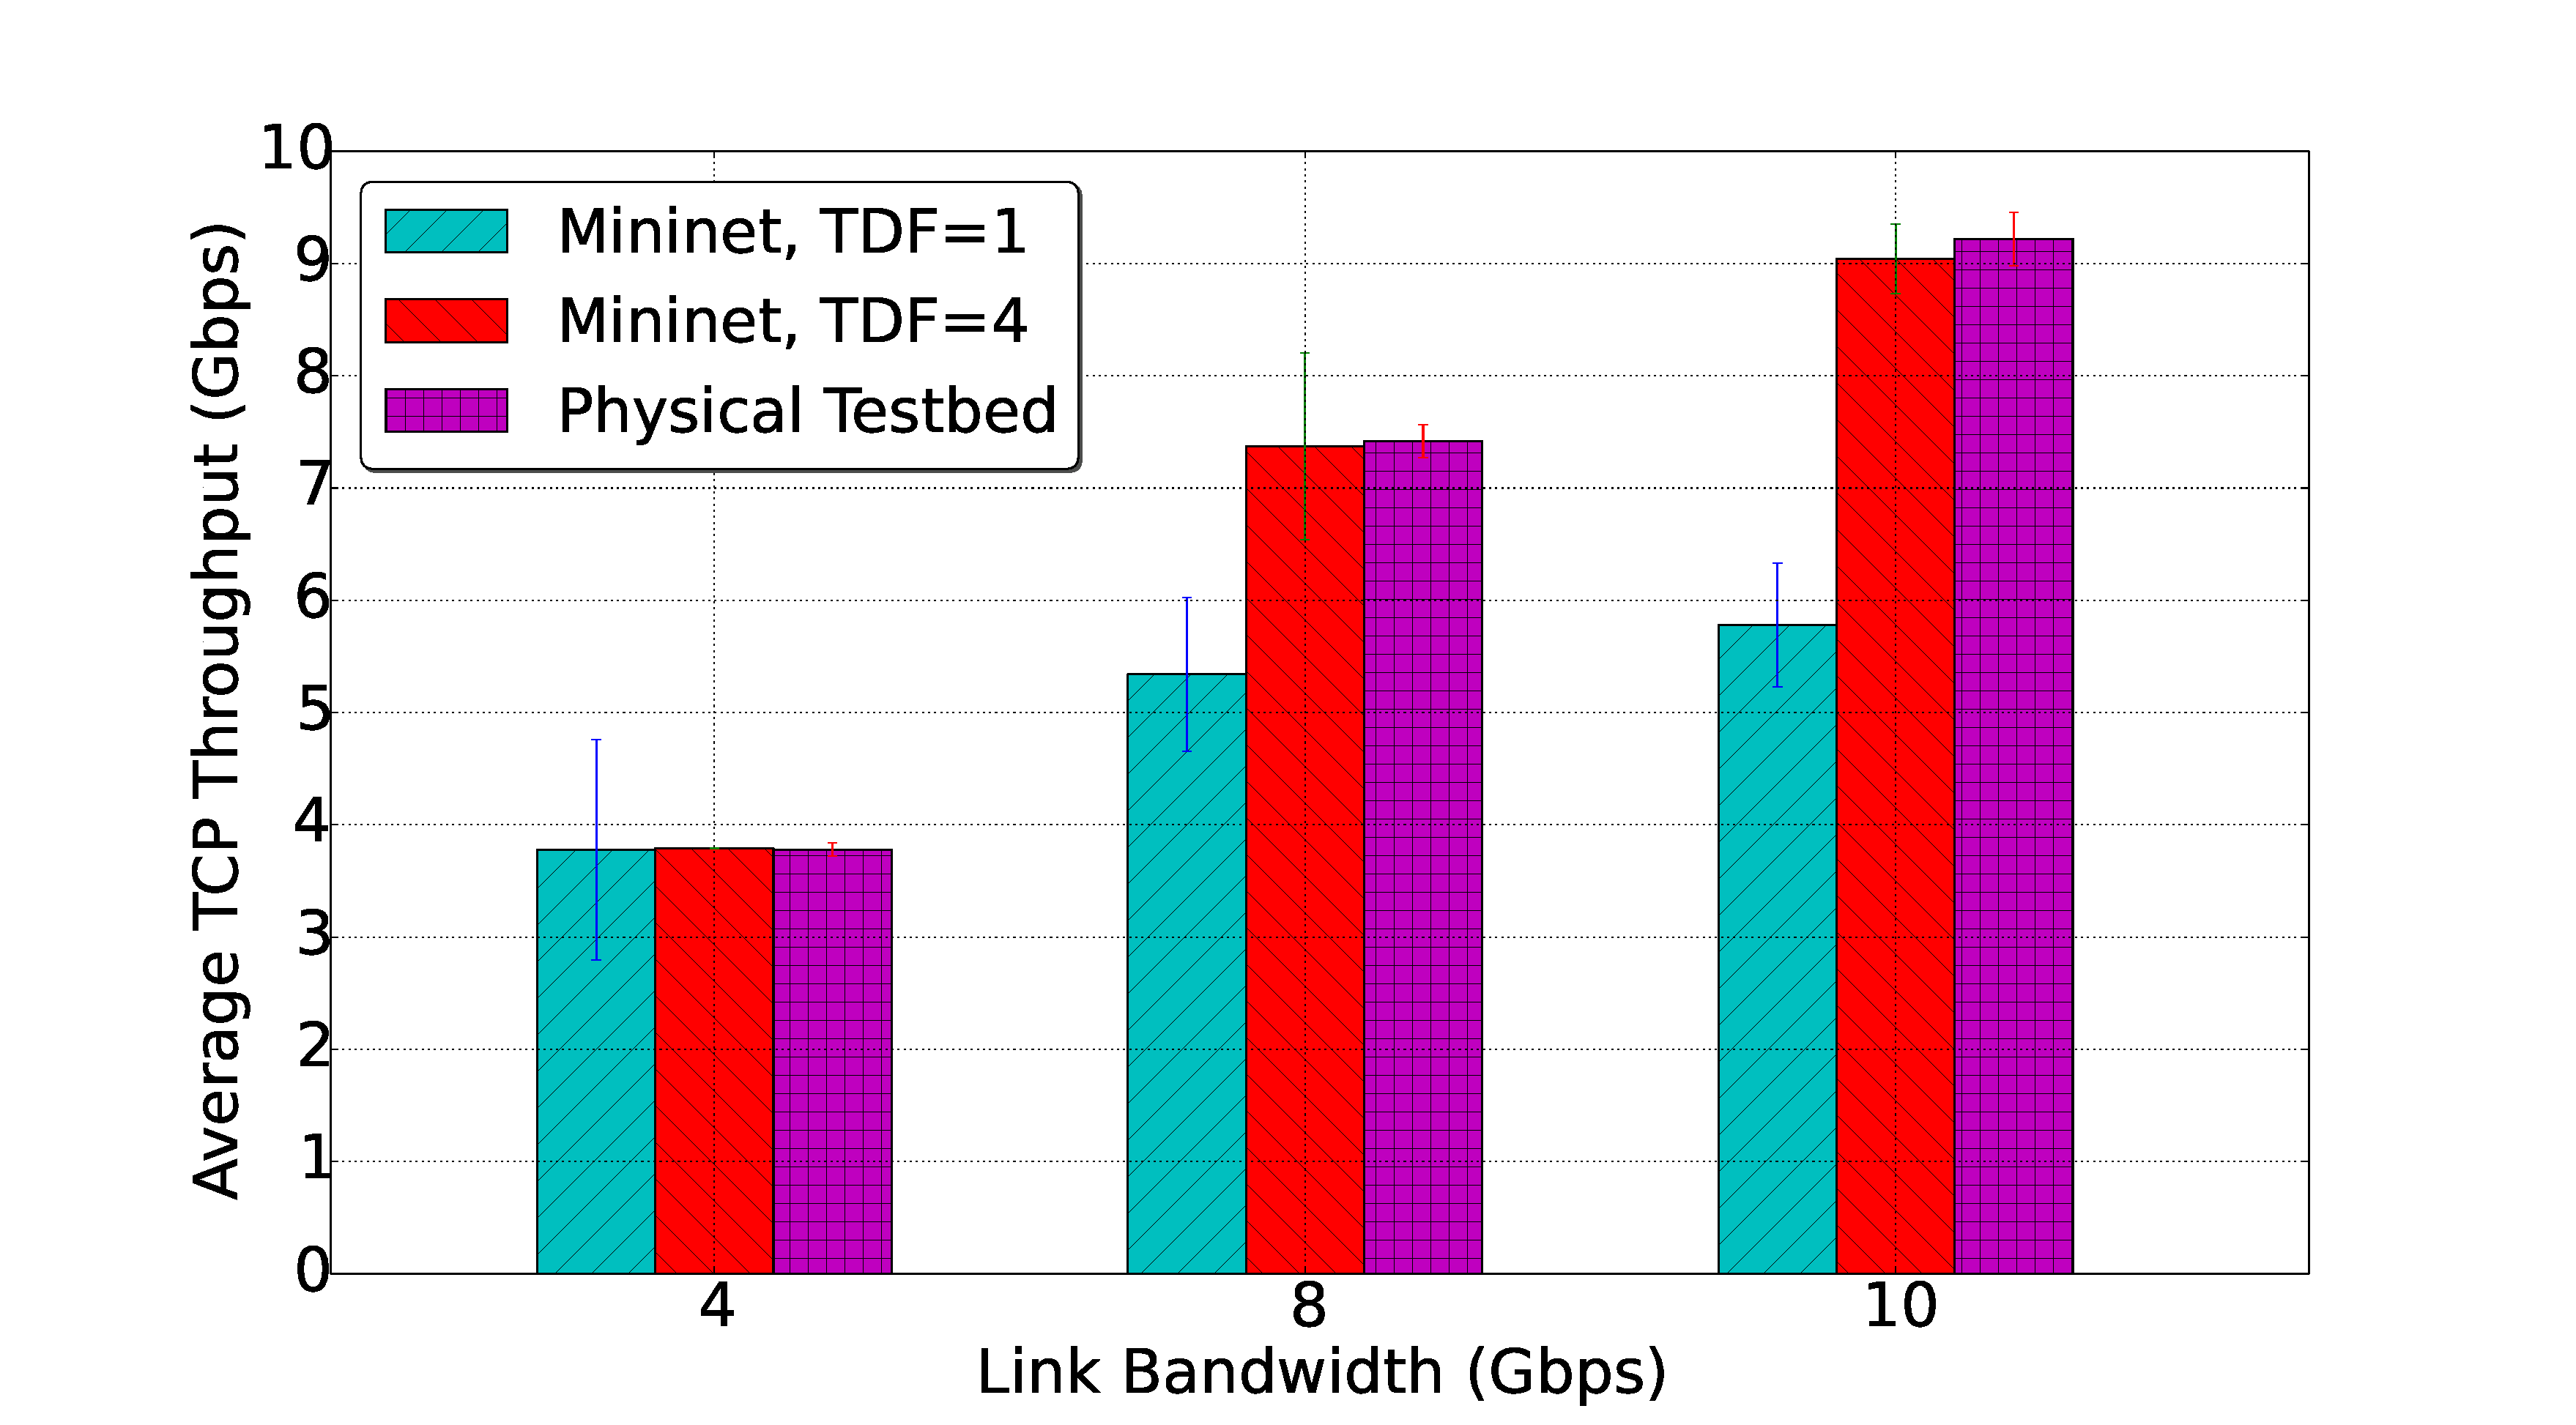
\epsfig{file=figures/Perf40SwDiffBw.eps, height=2.0in, width=3.4in}
		\label{Fig-Perf40SwDiffBw}
	}~
	\subfloat[\textbf{TCP Throughput with 10 Gbps Links}]
	{
		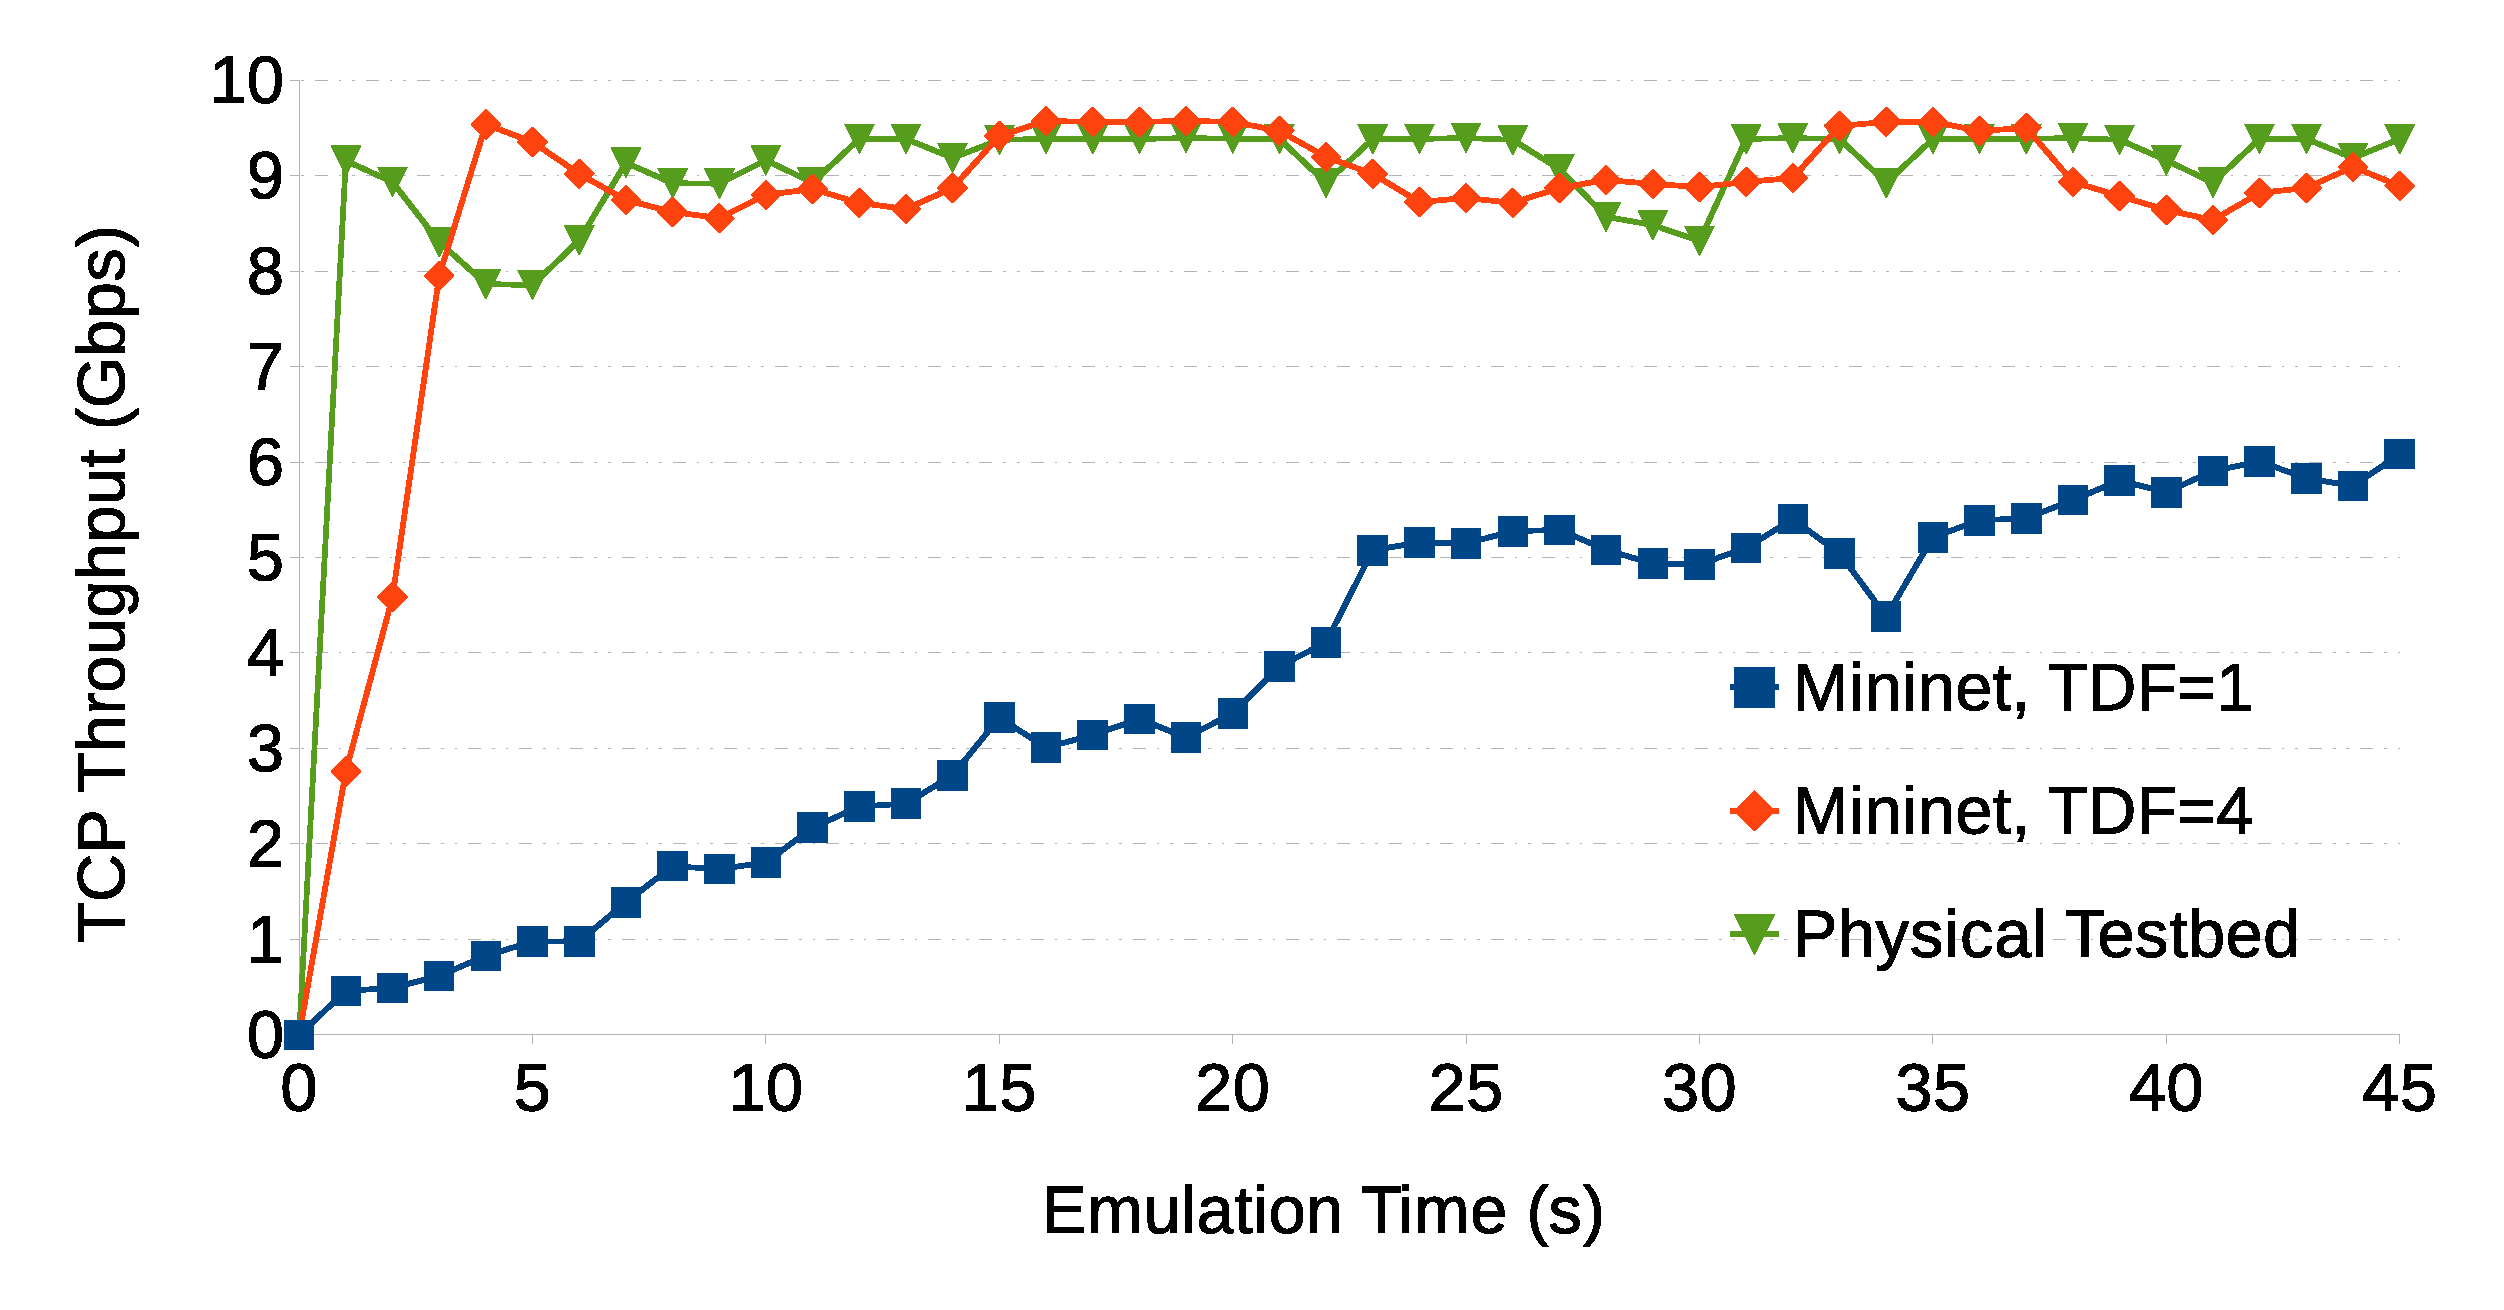
\epsfig{file=figures/Perf40Sw10GbLink.eps, height=1.8in, width=3.4in}
		\label{Fig-Perf40Sw10GbLink}
	}

\caption{\textbf{Fidelity Evaluation Experimental Results}}
\end{figure*}

\begin{figure*}
\centering
	%\subfloat[Mean \& Stdev of TCP Throughput.]{
	\subfloat[\textbf{TCP Throughput}]{
		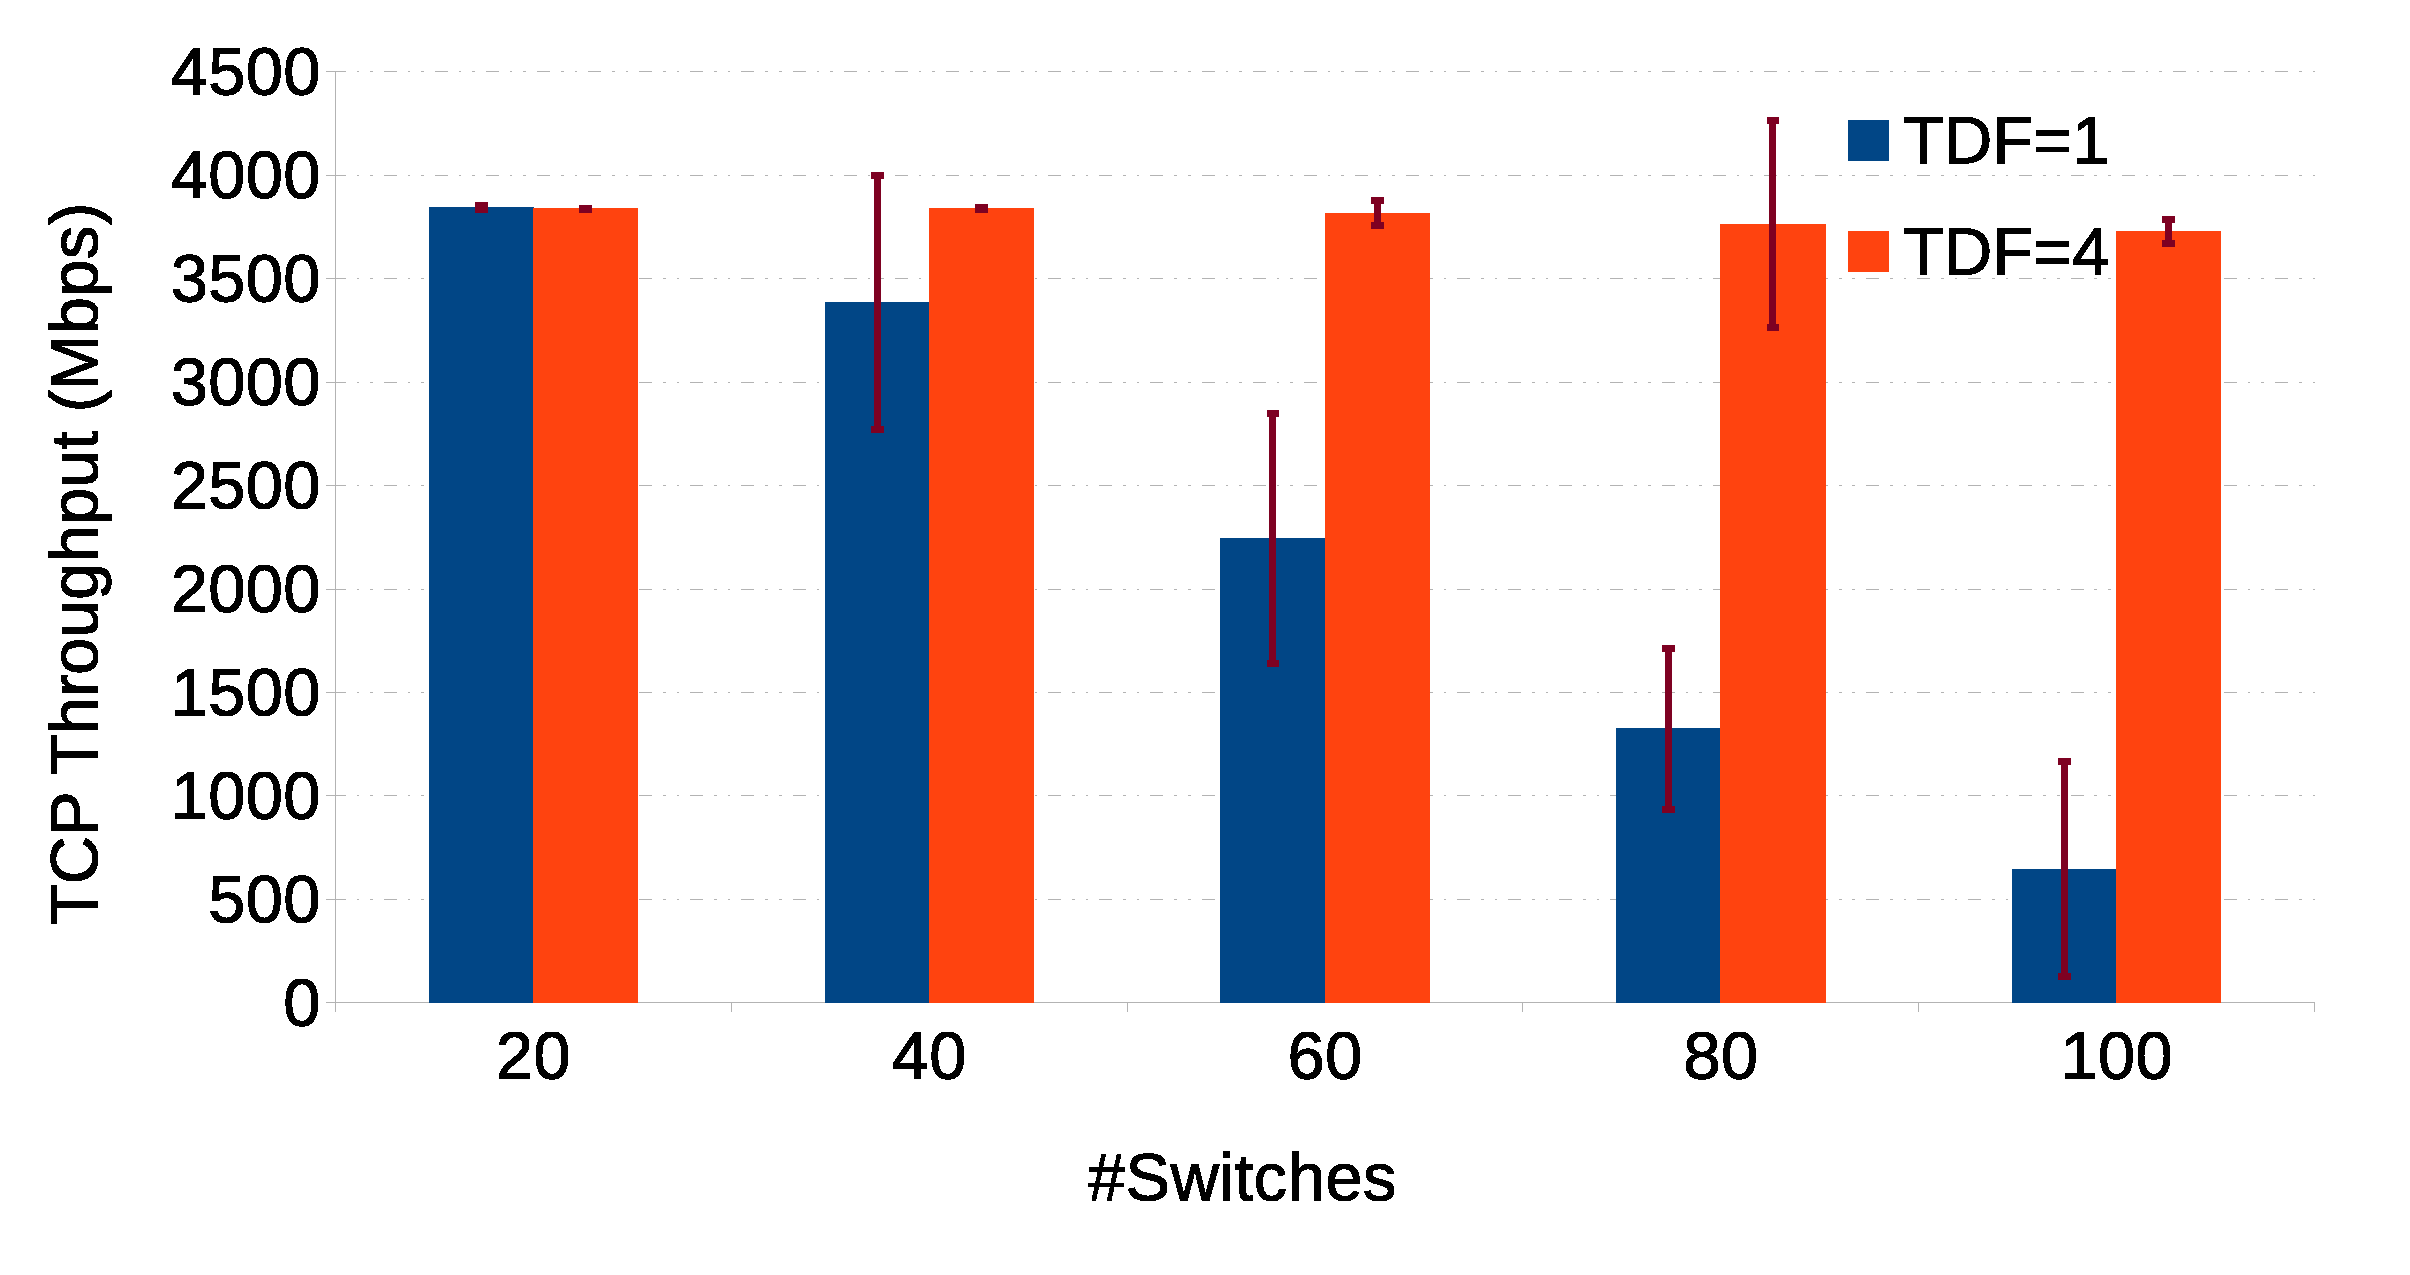
\epsfig{file=figures/ScaleDiff100Sw4GbLink.eps, height=2.0in, width=3.5in}
		\label{Fig-ScaleDiffSw4GbLink}
	}~
%	\subfloat[Scalability Limit Under Different TDFs.]
%	{	
%		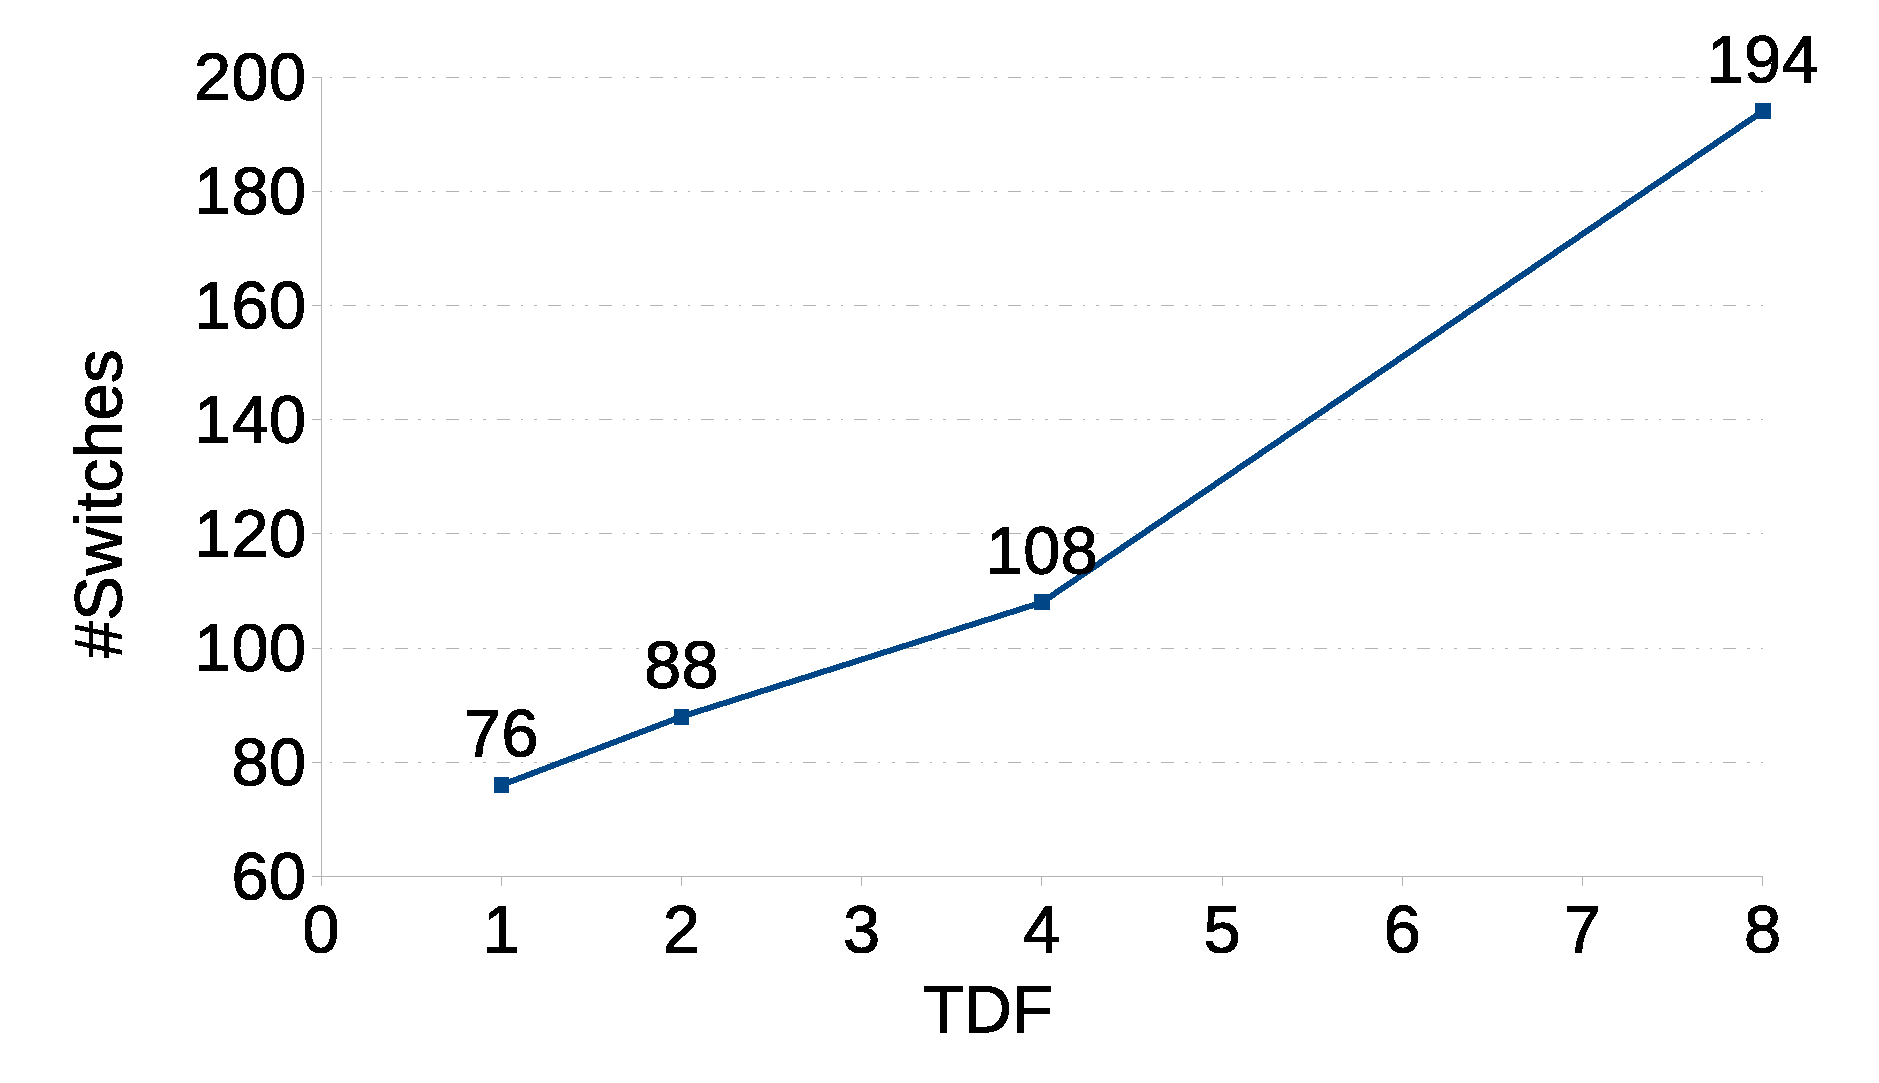
\epsfig{file=figures/ScaleSwThreshold.eps, height=2.0in, width=3.5in}
%		\label{Fig-ScaleSwThreshold}
%	}\\
	%\subfloat[Emulation Running Time.]
	\subfloat[\textbf{Emulation Running Time}]
	{
		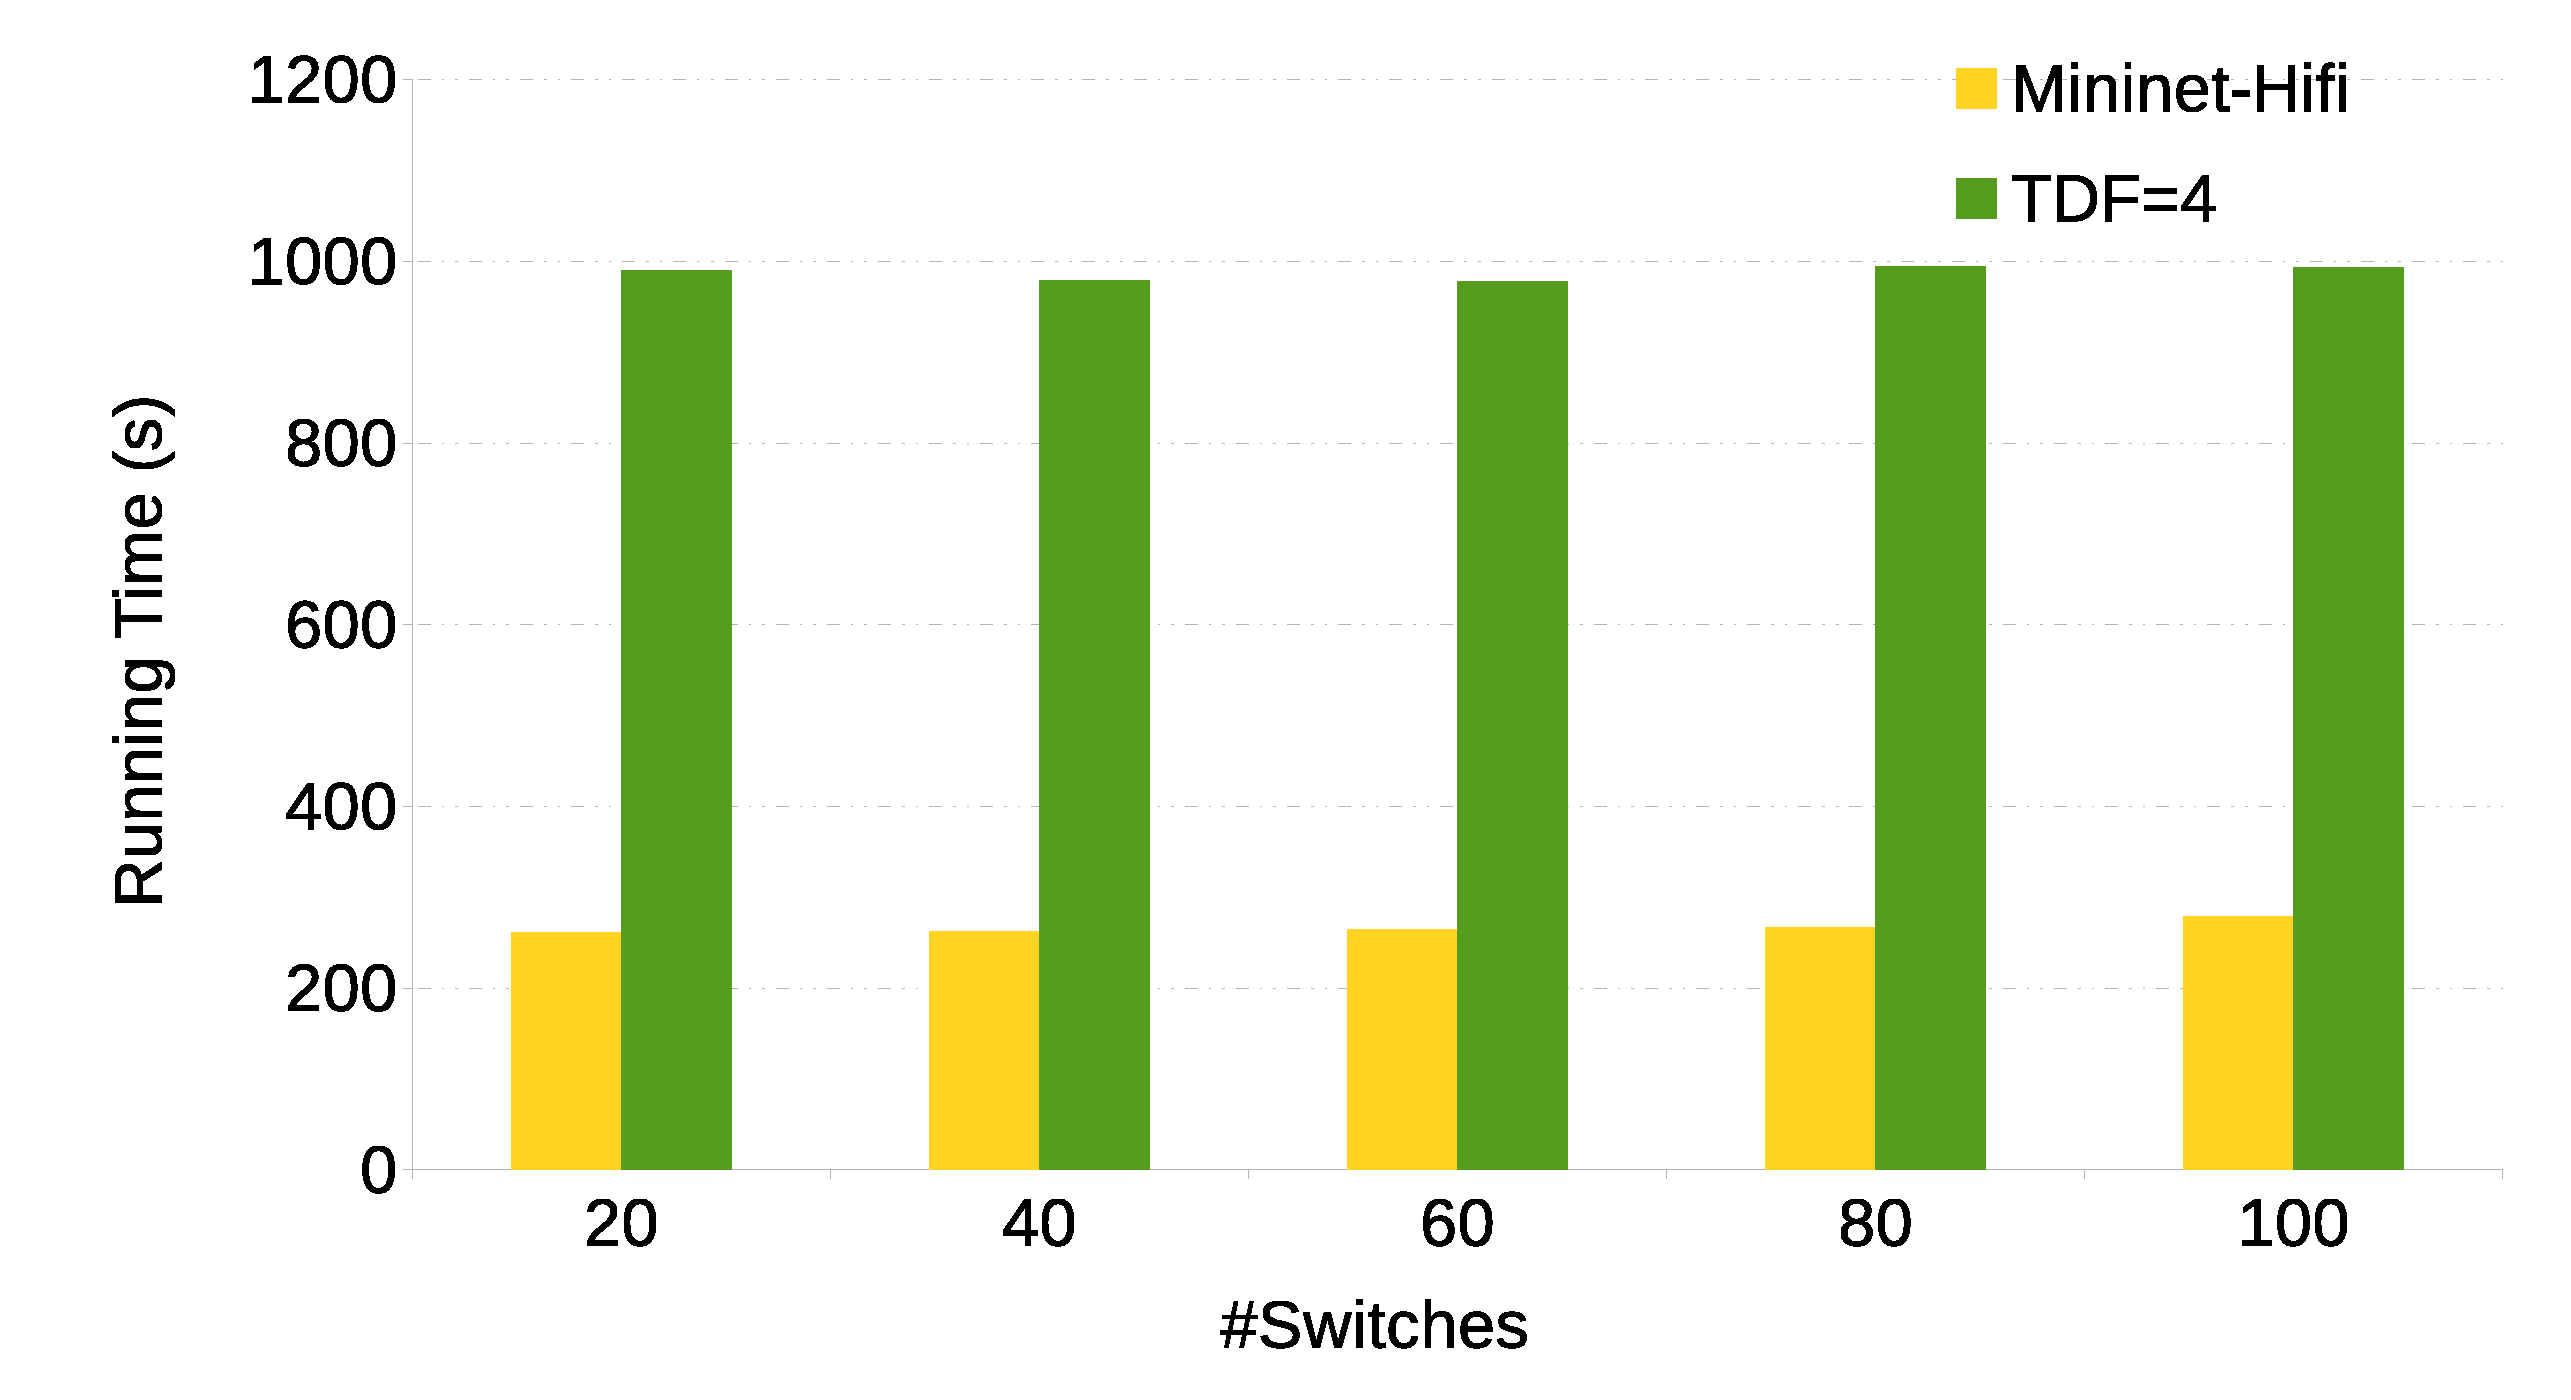
\epsfig{file=figures/ScaleTime100Sw4GbLink.eps, height=2.0in, width=3.5in}
		\label{Fig-ScaleTime}
	}%
\caption{\textbf{Scalability Evaluation Experimental Results}}
\end{figure*}

\paragraphb{Adaptive TDF Scheduling.}
We design a set of emulation experiments consisting of multiple TCP flows to evaluate the adaptive TDF scheduling algorithm. The network topology has a simple linear structure as shown in Figure \ref{Fig-LinearTopoExample} and consists of 100 hosts and 99 switches. All the links are of 100 Mbps bandwidth and 1 ms delay. We selected 5 non-overlap client-server pairs: \texttt{(h1, h20), (h21, h40), h(41, h60), h(61, h80), (h81, h100)}. The entire experiment was divided into three phases: (1) initially, transmit flow \texttt{(h1,h20)}, (2) after 50 seconds, transmit all five flows, and (3) after 150 seconds, stop all the transmissions except for flow \texttt{(h1,h20)}. The goal is to evaluate how our adaptive time dilation scheduler behaves under dynamic emulation workloads with the peak load exceeding Mininet's capability.
 
We ran the experiments in three cases. In case 1, TDF was set to 1 (i.e., no virtual time) and the adaptive virtual time scheduling was disabled. All flows' TCP throughputs measured by \texttt{iperf3} over time are plotted in Figure \ref{Fig-5FlowsNoVT}. 
%We also record the average CPU utilization of the emulation experiment, obtained by \texttt{MininetMonitor} (see Section \ref{Sub-Sec-ImplementMininet}), in Table \ref{Tab-CompareRunTime}. 
In case 2, we enabled the adaptive time dilation management system with TDF initially set to 1, and conducted the same emulation experiments. Figure \ref{Fig-5FlowsAdaptiveVT} plots the throughputs of all five flows. In case 3, we used a fixed TDF ($TDF = 11$) and disabled the adaptive virtual time scheduling. Results are shown in Figure \ref{Fig-5FlowsFixedVT}. We set $TDF=11$ because 11 was the largest value observed in the TDF changing history in case 2. In addition, the entire trace of the dynamic TDF in case 2 is plotted in Figure \ref{Fig-HistoryTDF}. We repeated each experiment for 5 times and observed very similar behaviors. All the time series reported in Figure \ref{Fig-Adaptive} were based on the data collected from one run. 

In phase 1, Mininet had sufficient system resources to emulate a single TCP flow \texttt{(h1, h21)}. Therefore, we observe the close-to-line-rate throughput, i.e., 100 Mbps, in all three cases. In phase 2, there were five concurrent flows in the network and each case demonstrated different behaviors. Note that those flows were non-overlap flows because they did not share any links or switches. Therefore, all five flows should achieve close-to-line-rate throughputs, i.e., 100 Mbps, in physical world applications.
In case 1, the throughputs of all five flows were very unstable as shown in Figure \ref{Fig-5FlowsNoVT}, which reflected the heavy resource contention in Mininet. In contrast, in case 3, all five flows have stable, close-to-100-Mbps throughputs because of the virtual time. In case 2, we observed disturbances in throughput at the beginning of phase 2, but the five flows quickly converged to the stable close-to-line-rate throughput because the adaptive TDF scheduler managed to compute the optimal TDF value. The details of TDF adjustment are depicted in Figure \ref{Fig-HistoryTDF}. In phase 3, the emulation returned back to a single flow \texttt{(h1, h21)}, and the measured throughputs were accurate in all three cases.
As indicated by Figure \ref{Fig-HistoryTDF}, our scheduler decreased the TDF value accordingly in case 2 to save emulation time in phase 3 while still preserving the fidelity. 

Table \ref{Tab-CompareRunTime} summarizes the execution time, the average TDF, and the rate of execution time in wall clock to the emulation time (200 seconds) of all three cases. 
%Note that in case 1 with no virtual time, the experiment lasted for 240 seconds. The overhead was not introduced by our scheduler nor by Mininet. //but emulation time != wall-clock time. 
We can see that case 3 ($TDF = 11$) is around 10 times slower than case 1 ($TDF = 1$) in order to guarantee fidelity. Our adaptive time dilation scheduler managed to reduce 46\% of the running time as compared to case 3 with little fidelity loss. 

\begin{figure*}
\centering
	\subfloat[\textbf{TCP Throughput without Virtual Time}]
	{
		{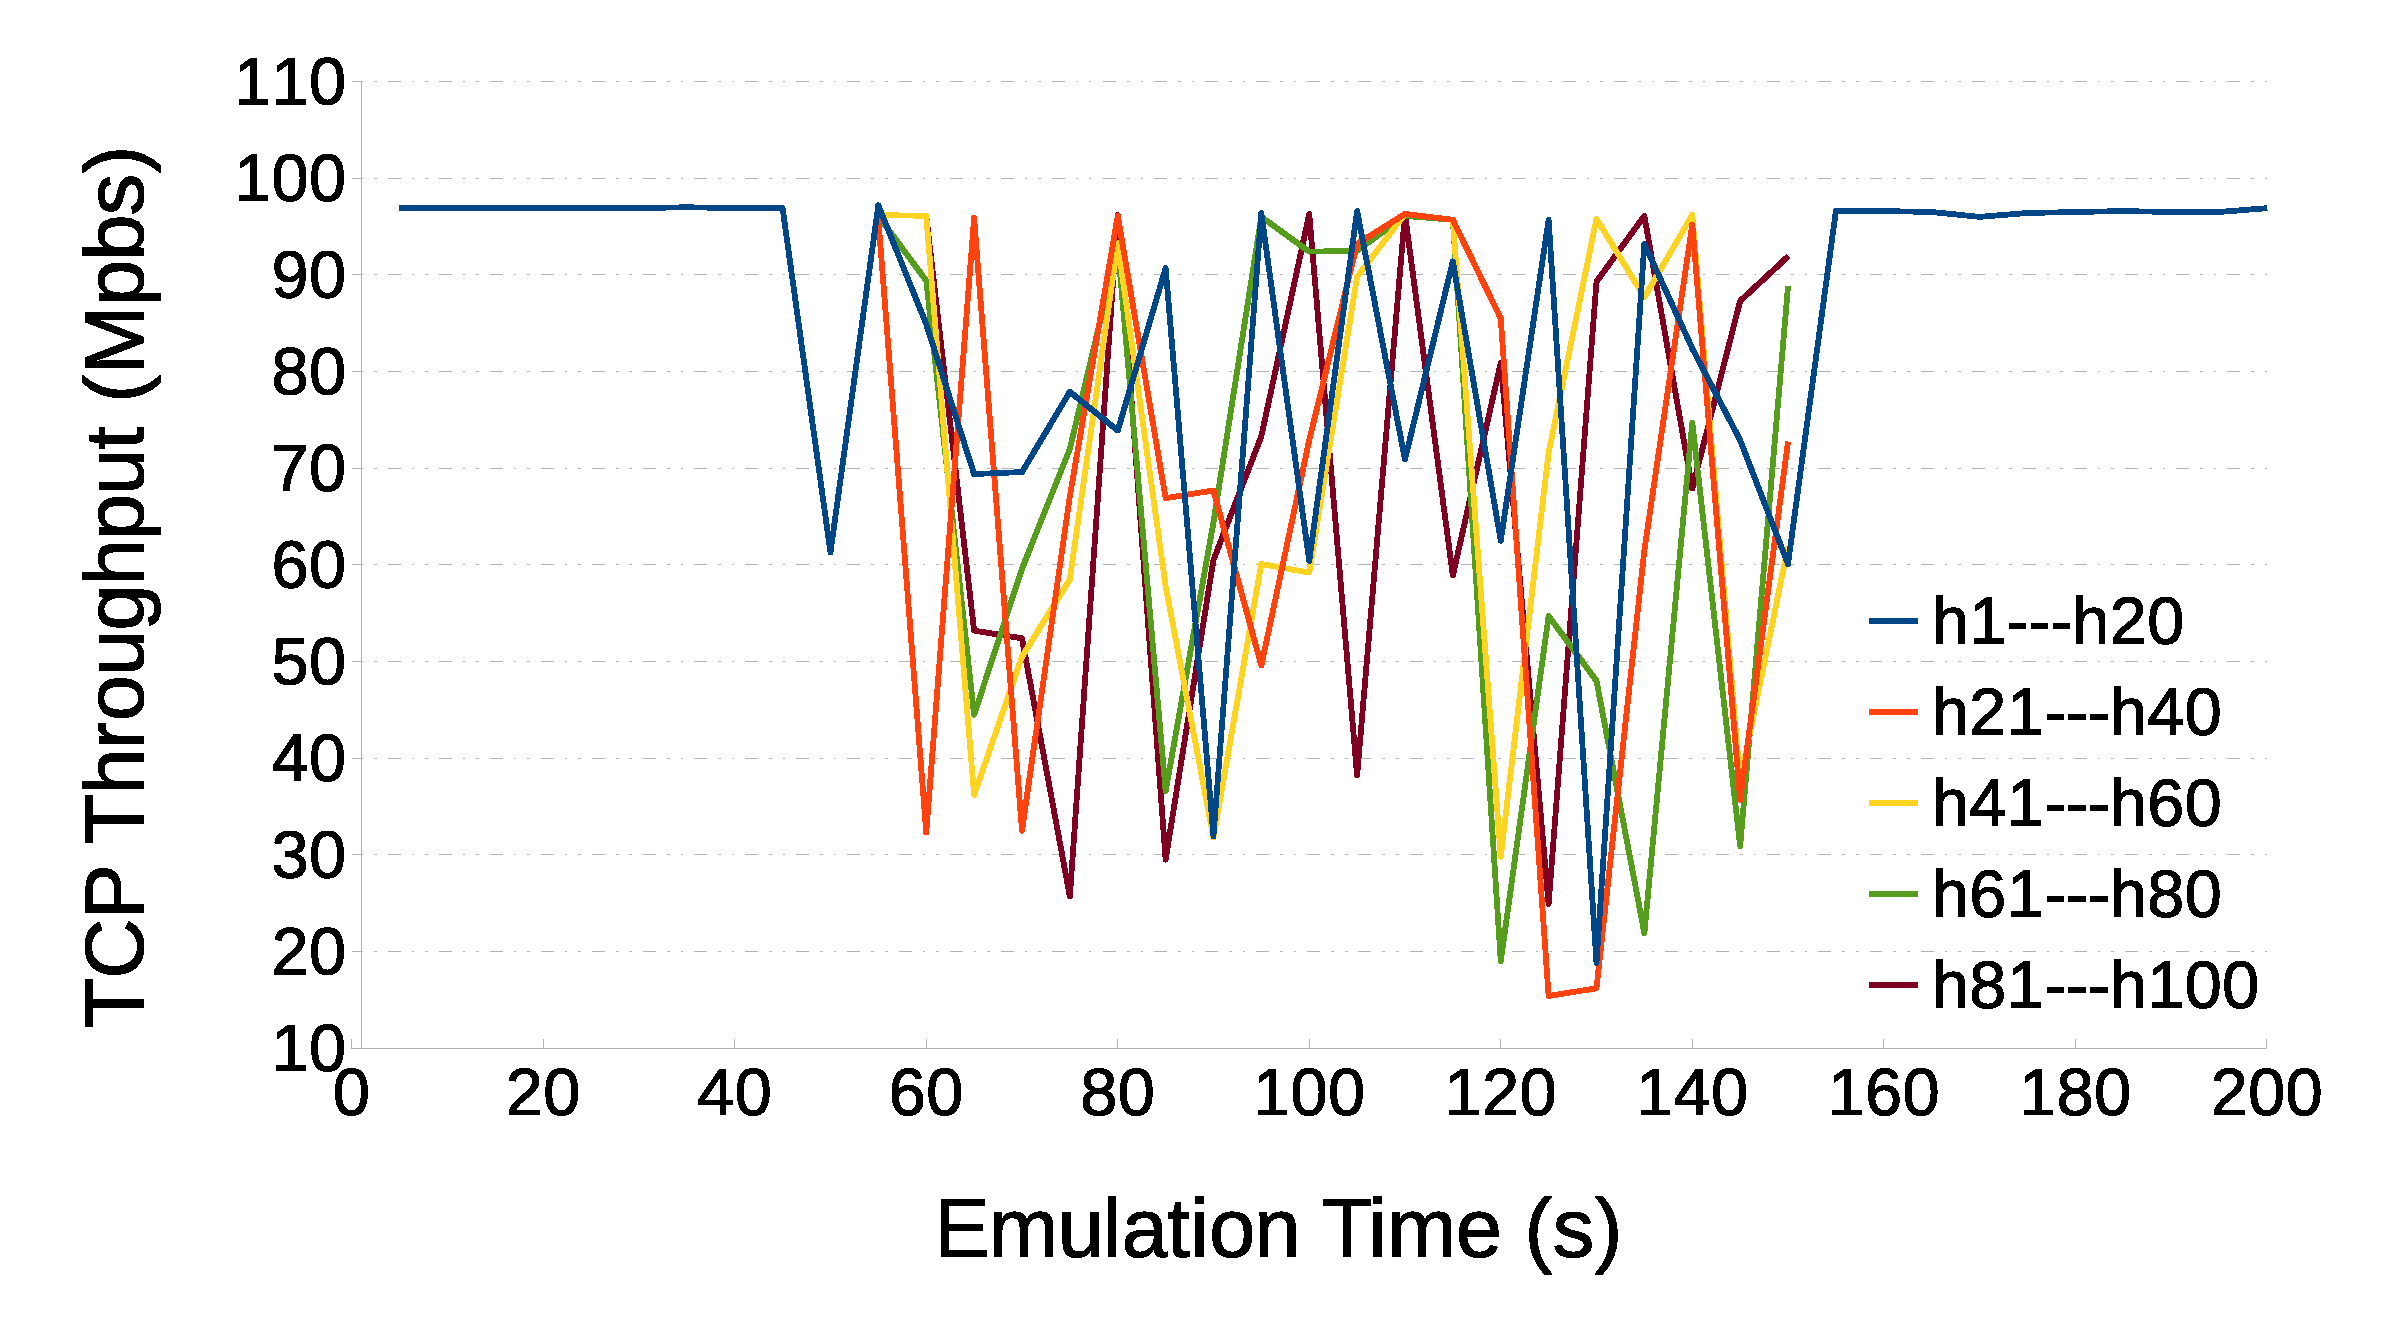
\epsfig{file=figures/5FlowsNoVT.eps, height=1.8in, width=3.3in}}
		\label{Fig-5FlowsNoVT}
	}~
	\subfloat[\textbf{TCP Throughput with Adaptive Time Dilation}]
	{
		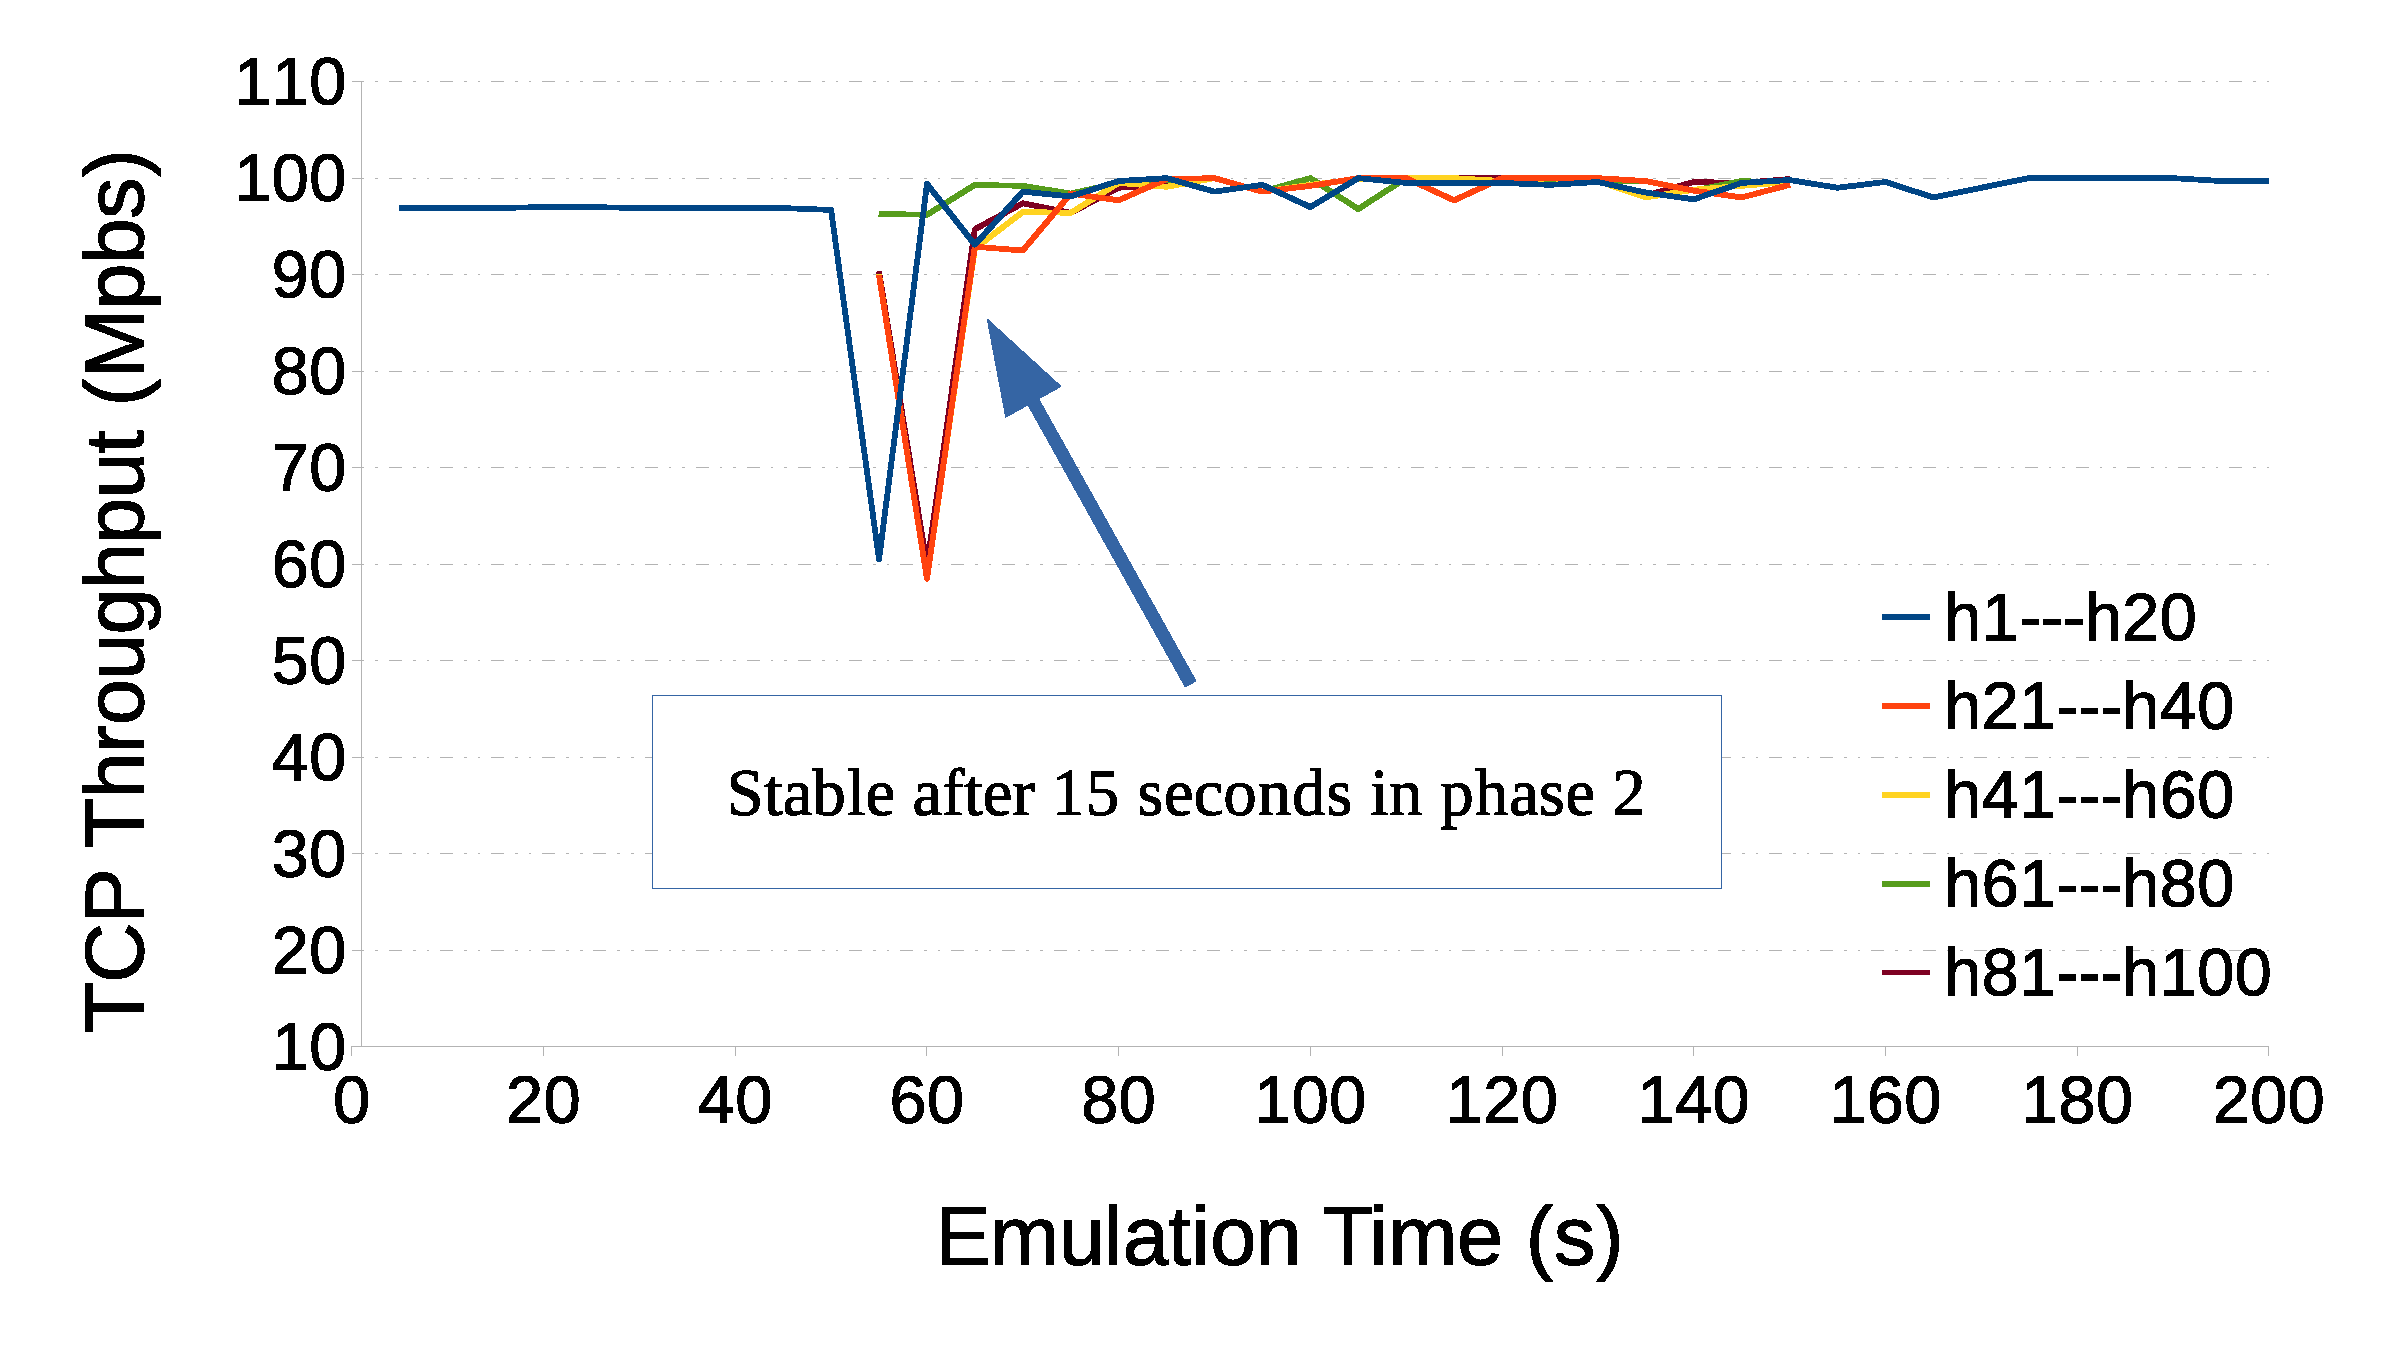
\epsfig{file=figures/5FlowsAdaptiveVT.eps, height=1.8in, width=3.3in}
		\label{Fig-5FlowsAdaptiveVT}
	}
	
	\subfloat[\textbf{TCP Throughput with Fixed Time Dilation (11)}]
	{
		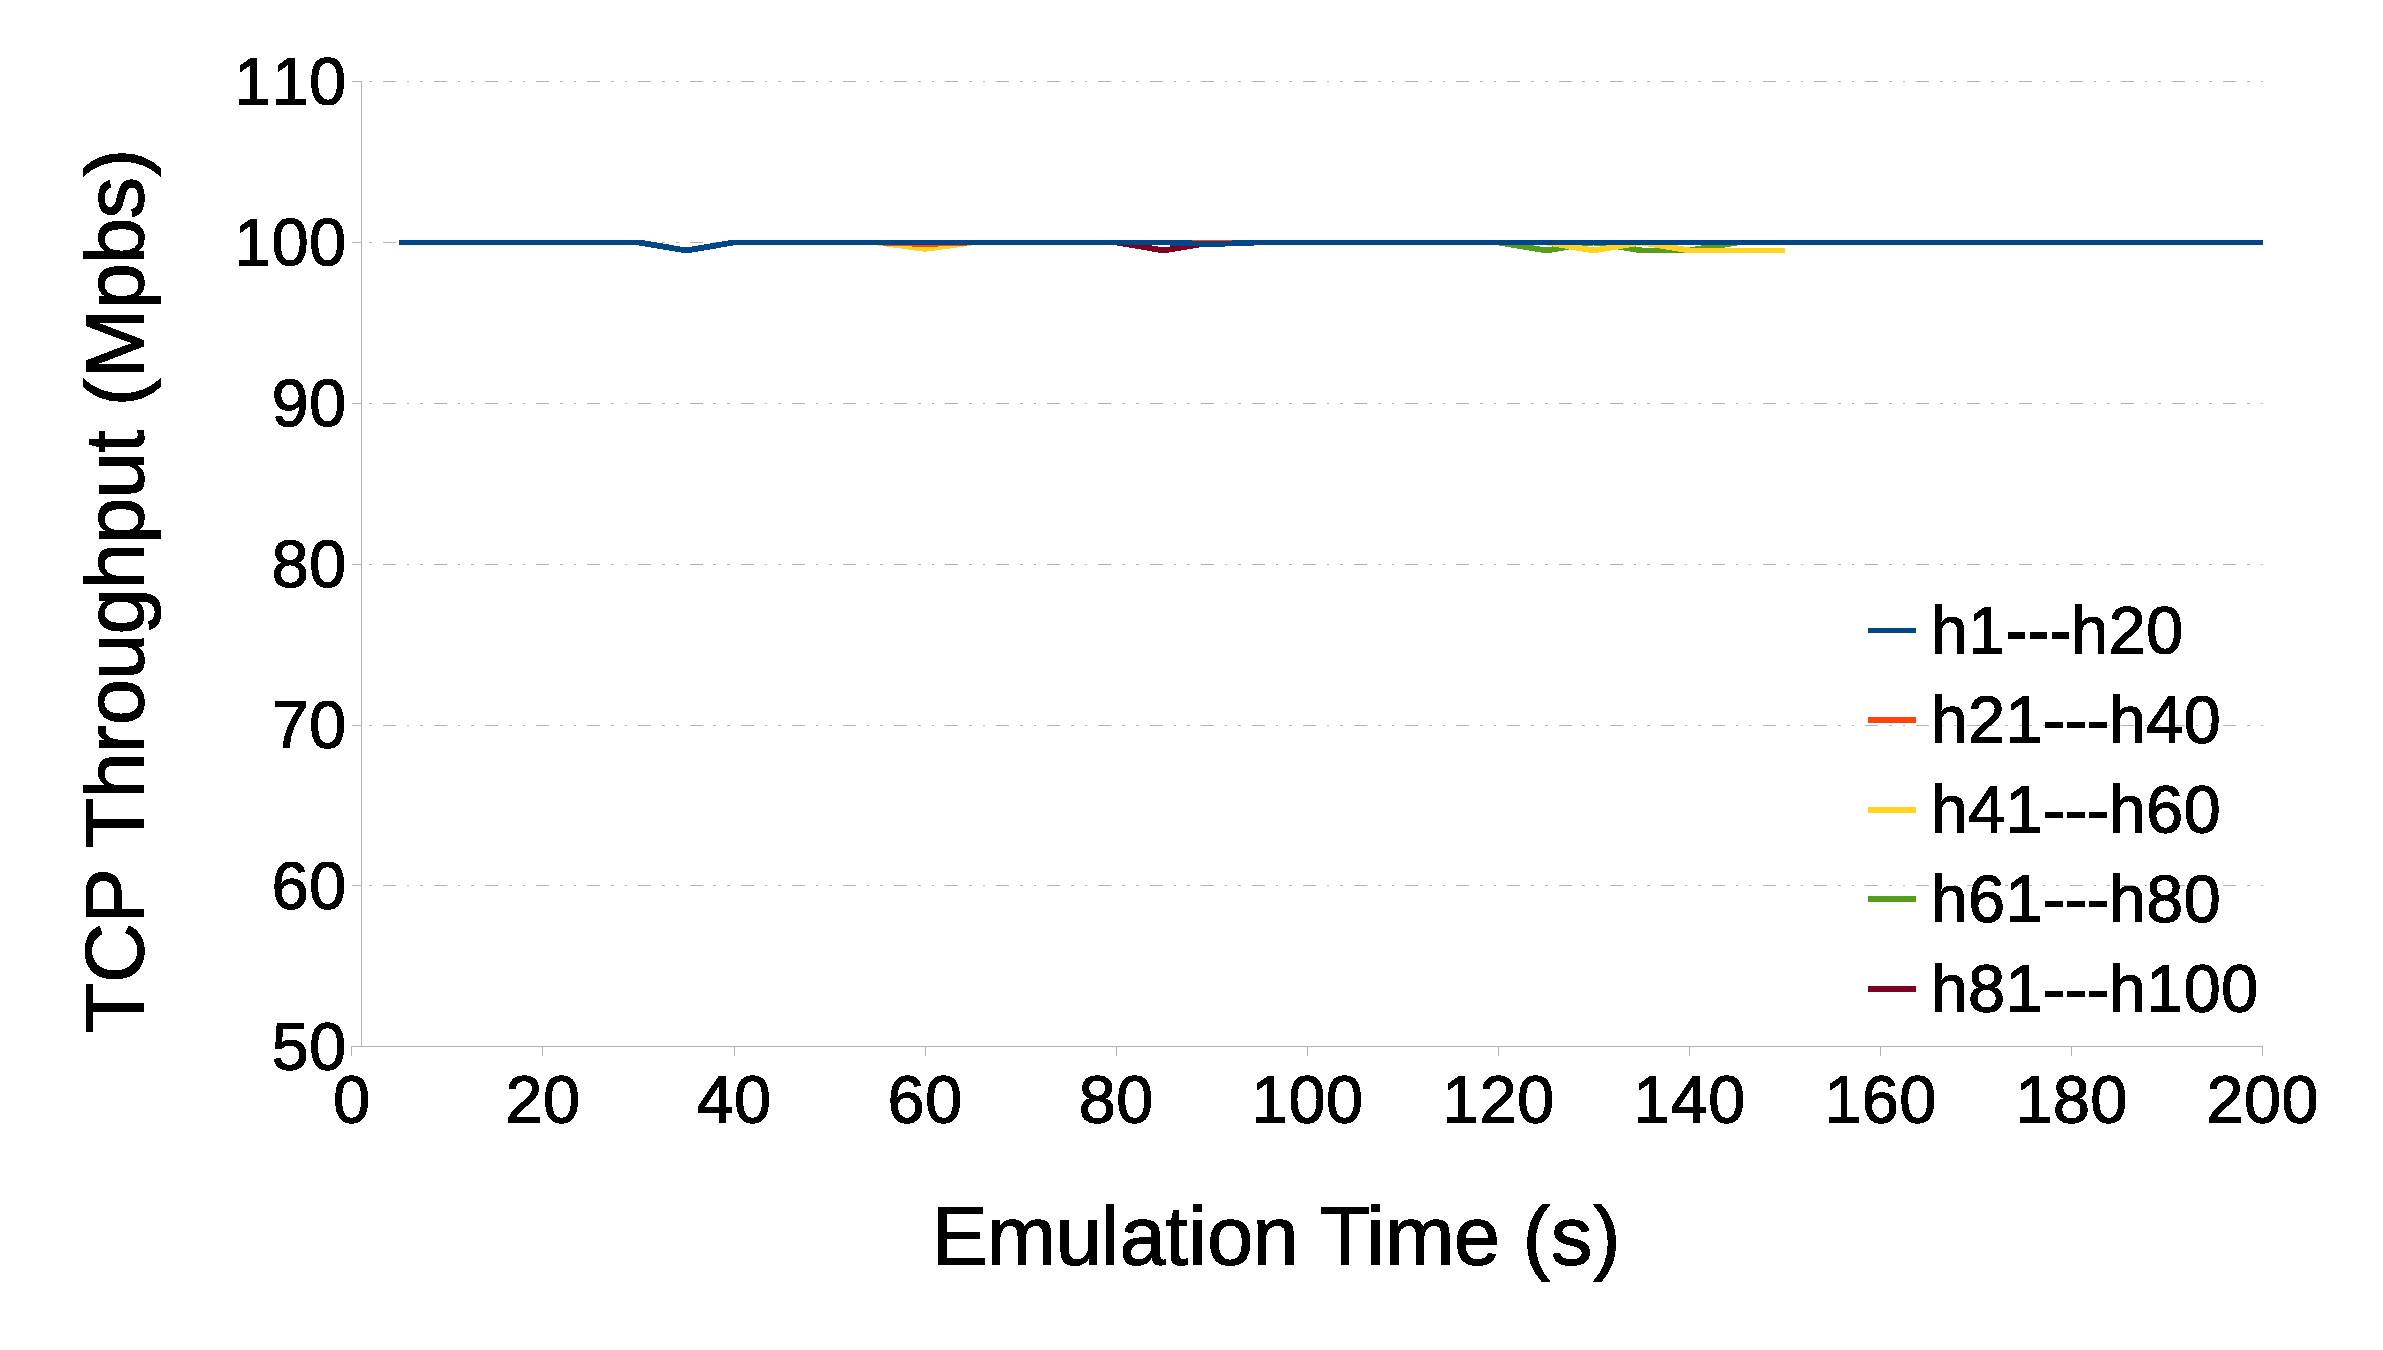
\epsfig{file=figures/5FlowsFixedVT.eps, height=1.8in, width=3.3in}
		\label{Fig-5FlowsFixedVT}
	}~
	\subfloat[\textbf{TDF Trace: Adaptive Virtual Time Scheduling}]
	{
		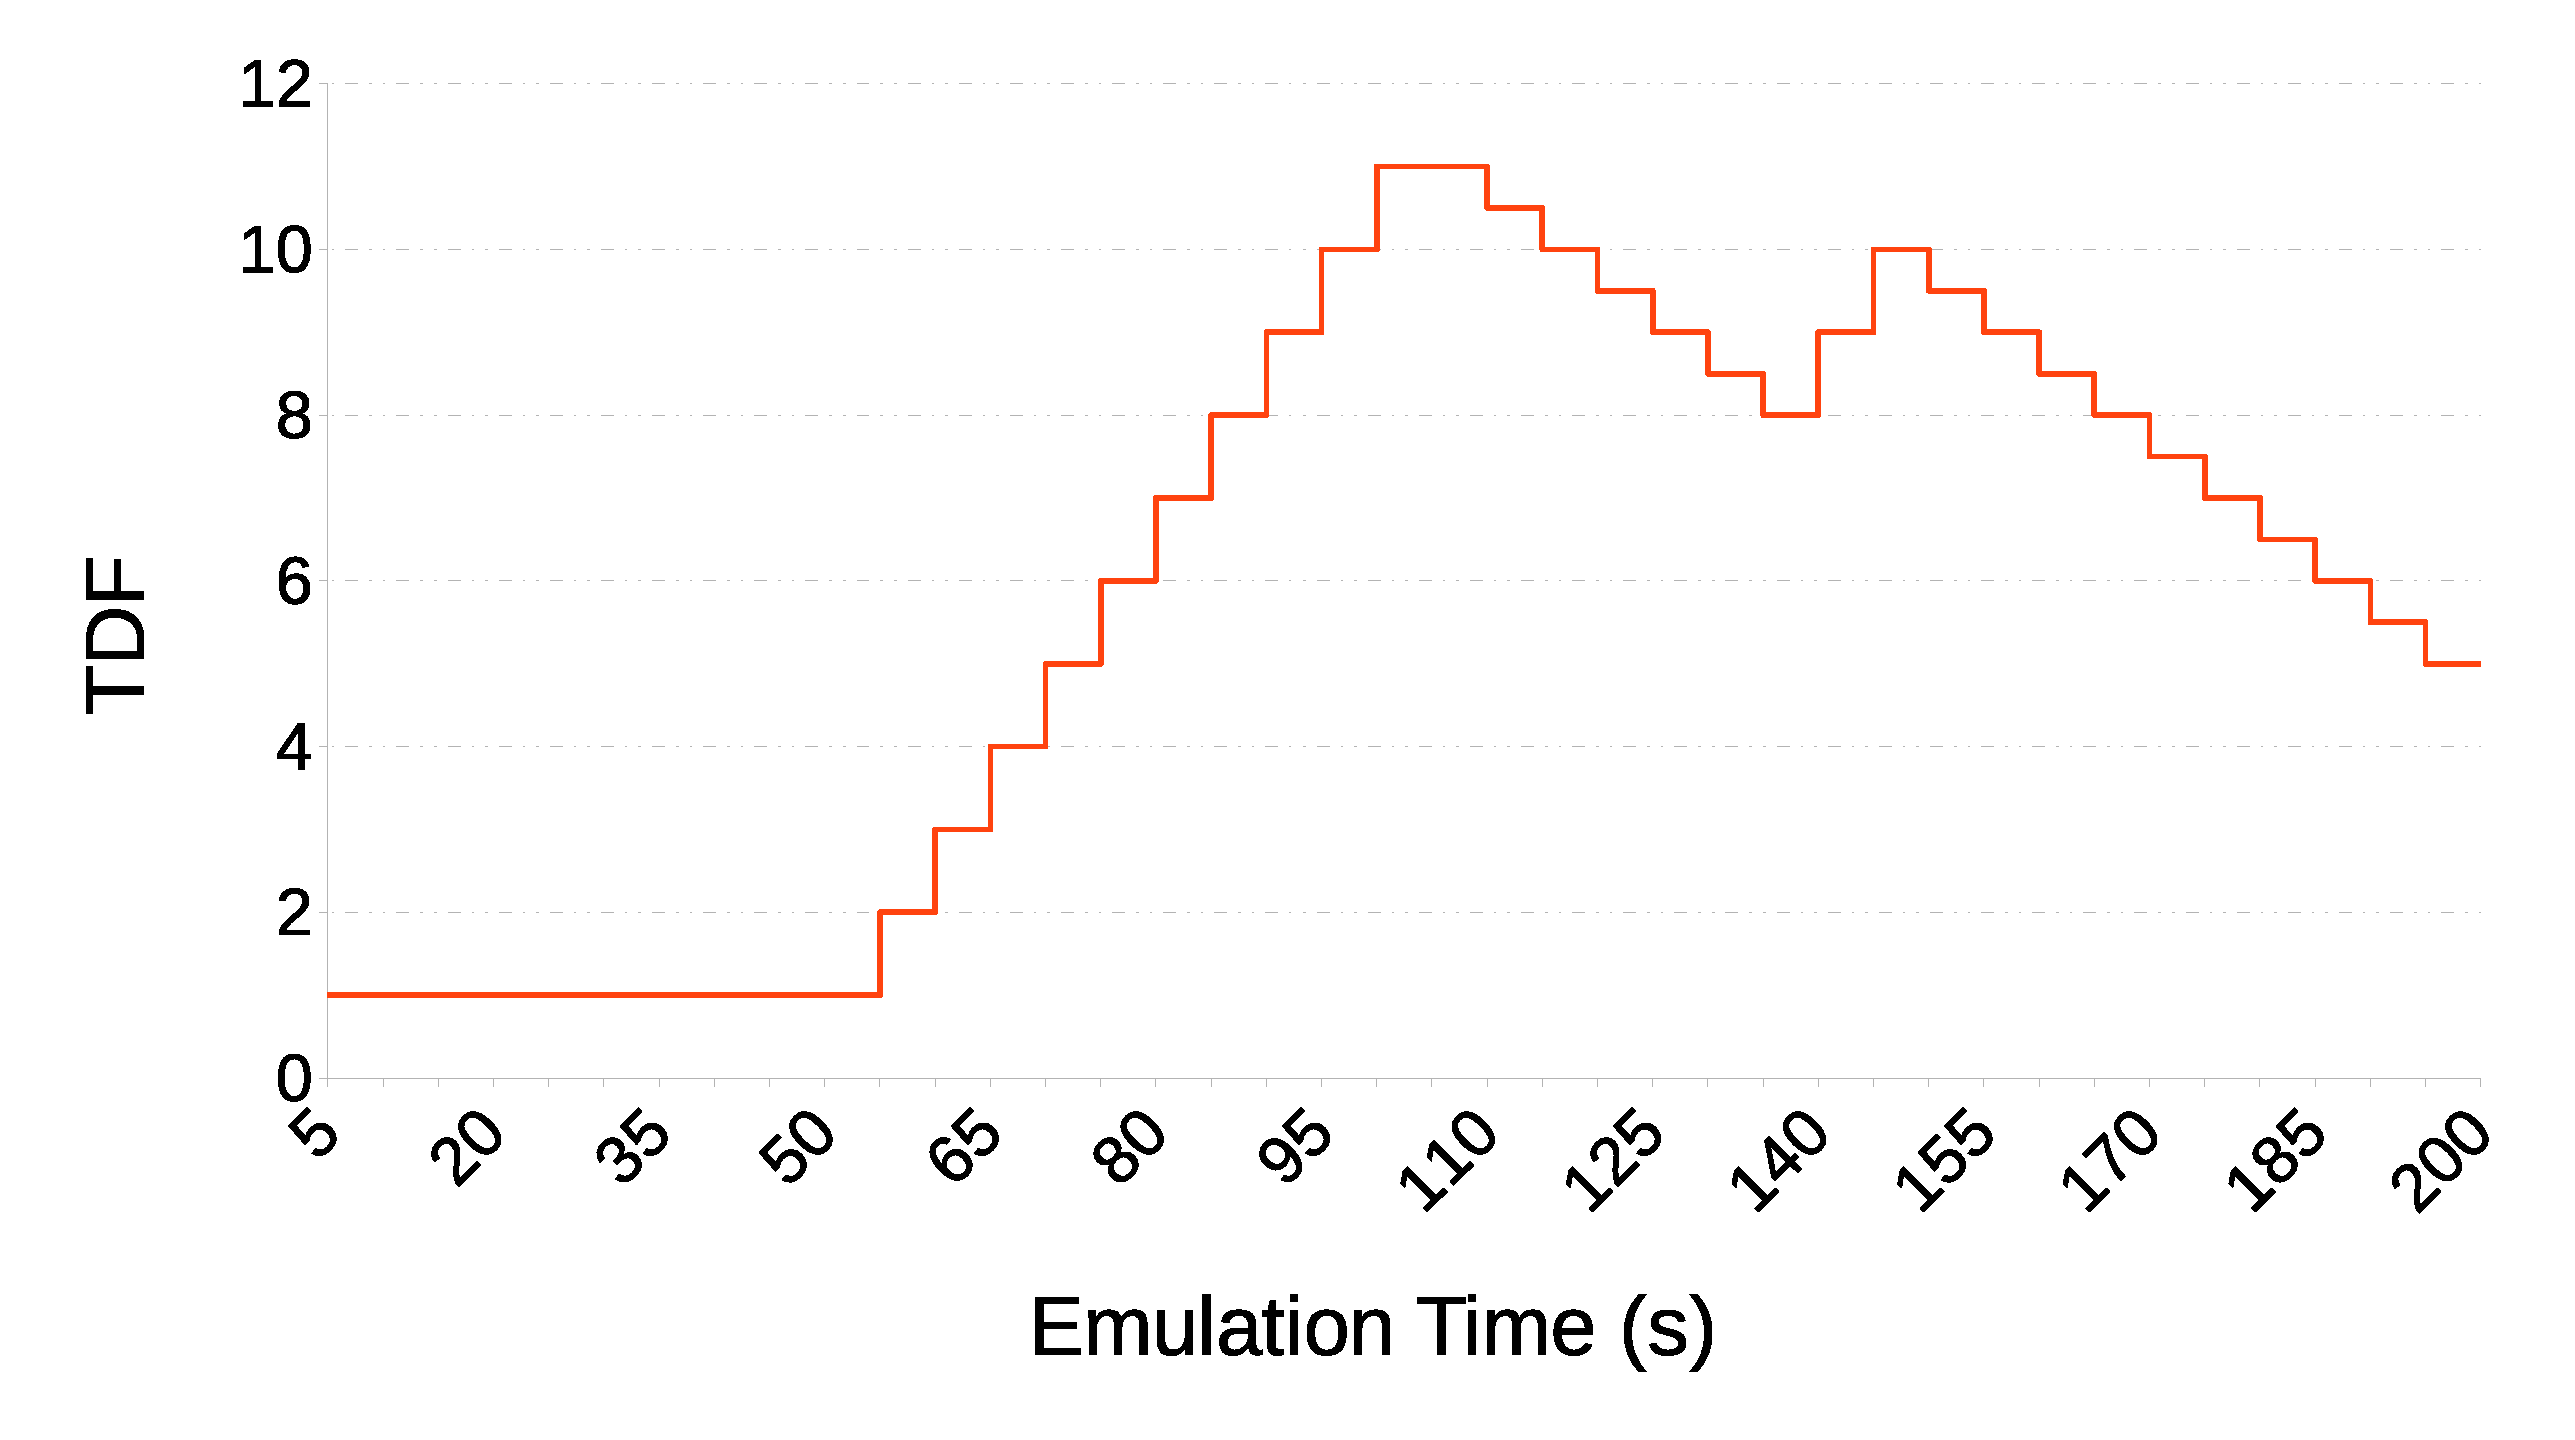
\epsfig{file=figures/5FlowsHistoryTDF.eps, height=1.8in, width=3.3in}
		\label{Fig-HistoryTDF}
	}
\caption{\textbf{Experimental Results: Adaptive Virtual Time Scheduling Evaluation}}
\label{Fig-Adaptive}
\end{figure*}

\begin{table*}
\centering
\caption{\textbf{Comparison of Emulation Execution Time}}
\begin{tabular}{|c|c|c|c|c|} 
\hline
 & No Virtual Time & Adaptive Virtual Time & Fixed Virtual Time \\ 
\hline
Running Time (s)  & 240.730 & 1332.242 & 2434.910 \\ 
\hline
Average TDF & 1.000 & 5.900 & 11.000 \\ 
\hline
%Slow Down Ratio & 1.204 & 5.534 & 10.115 \\
Slow Down Ratio & 1.000 & 5.534 & 10.115 \\
%\hline
%AVG. CPU\% & 31.968 & 28.287 & 20.376 \\ 
%\hline
%STDEV. CPU\% & 10.915 & 7.175 & 4.173 \\ 
\hline
\end{tabular}
\label{Tab-CompareRunTime}
\end{table*}



%\subsection{System Overhead}
\paragraphb{System Overhead.}
Our virtual time system introduces overhead with the following two reasons: (1) the computation cost in Algorithm \ref{Alg-DilateTimeKeeping} and (2) the pauses of emulation when changing containers' TDFs. We measured both types of overhead and report the results in Table \ref{Tab-Overhead}.

First, we invoked both non-dilated and dilated \texttt{gettimeofday} 10,000,000 times from a user space application. The average overhead for one dilated \texttt{gettimeofday} is 0.013 microseconds.  We then used \texttt{strace} to count the number of invocations for \texttt{gettimeofday} in a 60-second \texttt{iperf3} run on both the server and the client. The total overhead is 18,145 microseconds after tracing 1,397,829 calls, which is about 0.03\% of the 60-second experiment. 
Actually, \texttt{iperf3} intensively invokes \texttt{gettimeofday}, because its timer is designed to exhaustively inquiry the OS time. The overhead amount will be even less for many other network applications. We also repeatedly changed a process's TDF 10,000,000 times using another test program. The average pause time was 0.063 microseconds, which is reasonably small. Since the number of TDF changes issued by the current adaptive TDF scheduling algorithm is a few orders of magnitude less than the number of calls to \texttt{gettimeofday} (e.g., only 14 TDF transitions occurred per host over the period of 1,332 seconds in the earlier adaptive TDF experiment), that overhead is also negligible.

\section{Case Study: Evaluation of ECMP in Data Center Networks}
\label{Sec-CaseStudy}
Network emulation testbeds are widely used to test and evaluate designs of network applications and protocols with the goal of discovering design limitations and implementation faults before the real system deployment. In this section, we present a case study to demonstrate how our virtual-time-enabled Mininet has been utilized to reproduce and validate the limitations of the equal-cost multi-path (ECMP) routing strategy in a data center network.

Many modern data center networks employ multi-rooted hierarchical tree topologies, and therefore ECMP-based protocols \cite{ECMP} are commonly used in data center networks for load-balancing traffic over multiple paths. When an ECMP-enabled switch has multiple next-hops on the best paths to a single destination, it selects the forwarding path by performing a modulo-N hash over the selected fields of a packet's header to ensure per-flow consistency. The key limitation of ECMP is that the communication bottleneck would occur when several large and long-lived flows collide on their hash and being forwarded to the same output port \cite{Hedera}. We borrowed the experiment scenario on a physical testbed described in \cite{Hedera}, and created a set of emulation experiments in Mininet to demonstrate the limitation of ECMP. We built a fat-tree topology in Mininet as shown in Figure \ref{Fig-FattreeTopoExample}, and generated stride-style traffic patterns. Note that stride($i$) means that a host with index $x$ sends to the host with index $(x + i)$ mod $n$, where $n$ is the number of hosts \cite{Hedera}. The hash-based ECMP mechanism is provided by the RipL-POX SDN controller \cite{RipLPox}. The Mininet code was developed with reference to \cite{ReproNetReserch}. In all the following experiments, we set up 8 sender-receiver pairs transmitting stride-pattern traffic flows using step 1 and 4.

\begin{figure*}[htbp]
\centering
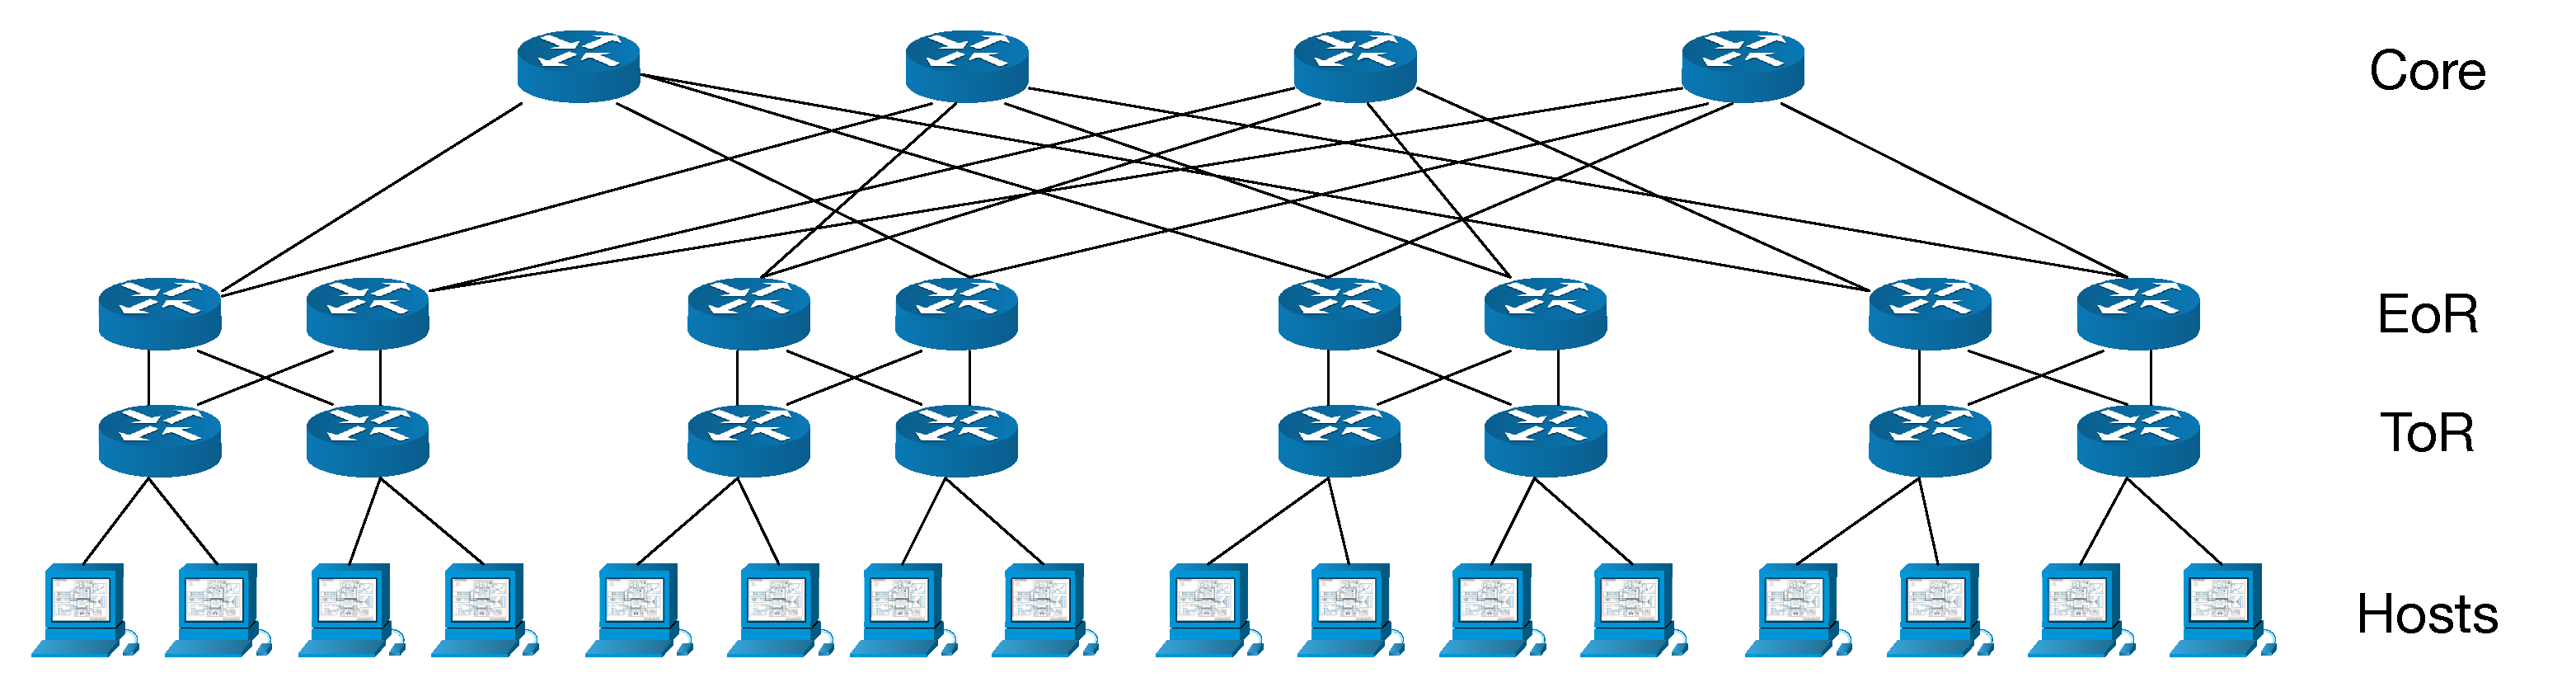
\epsfig{file=figures/TopoFatTreeExample.eps, height=1.4in, width=4.8in}
\caption{\textbf{A Data Center Network with a Degree-4 Fat Tree Topology}}
\label{Fig-FattreeTopoExample}
\end{figure*}

We first set all the link bandwidth (switch-to-switch and switch-to-host) to 100 Mbps, and conducted each experiment over three independent runs. The average throughput of 8 TCP flows was plotted in Figure \ref{Fig-FatTreeAvgBw100M}, and each individual flow's throughput (24 in total) was plotted in Figure \ref{Fig-FatTreeIndividualBw100M}. The limitation of ECMP presented in \cite{Hedera} was clearly observed. When many conflicting flows occurred with stride-4 flow patterns, the average throughput in the fat-tree network dramatically fell below 30 Mbps with up to 75\% throughput drop. As shown in Figure \ref{Fig-FatTreeIndividualBw100M}, every flow's throughput was largely affected by the hash collision limitation of ECMP in the stride-4 scenario.

\begin{figure*}[htbp]
\centering
	\subfloat[\textbf{Average TCP Flow Throughput}]{
		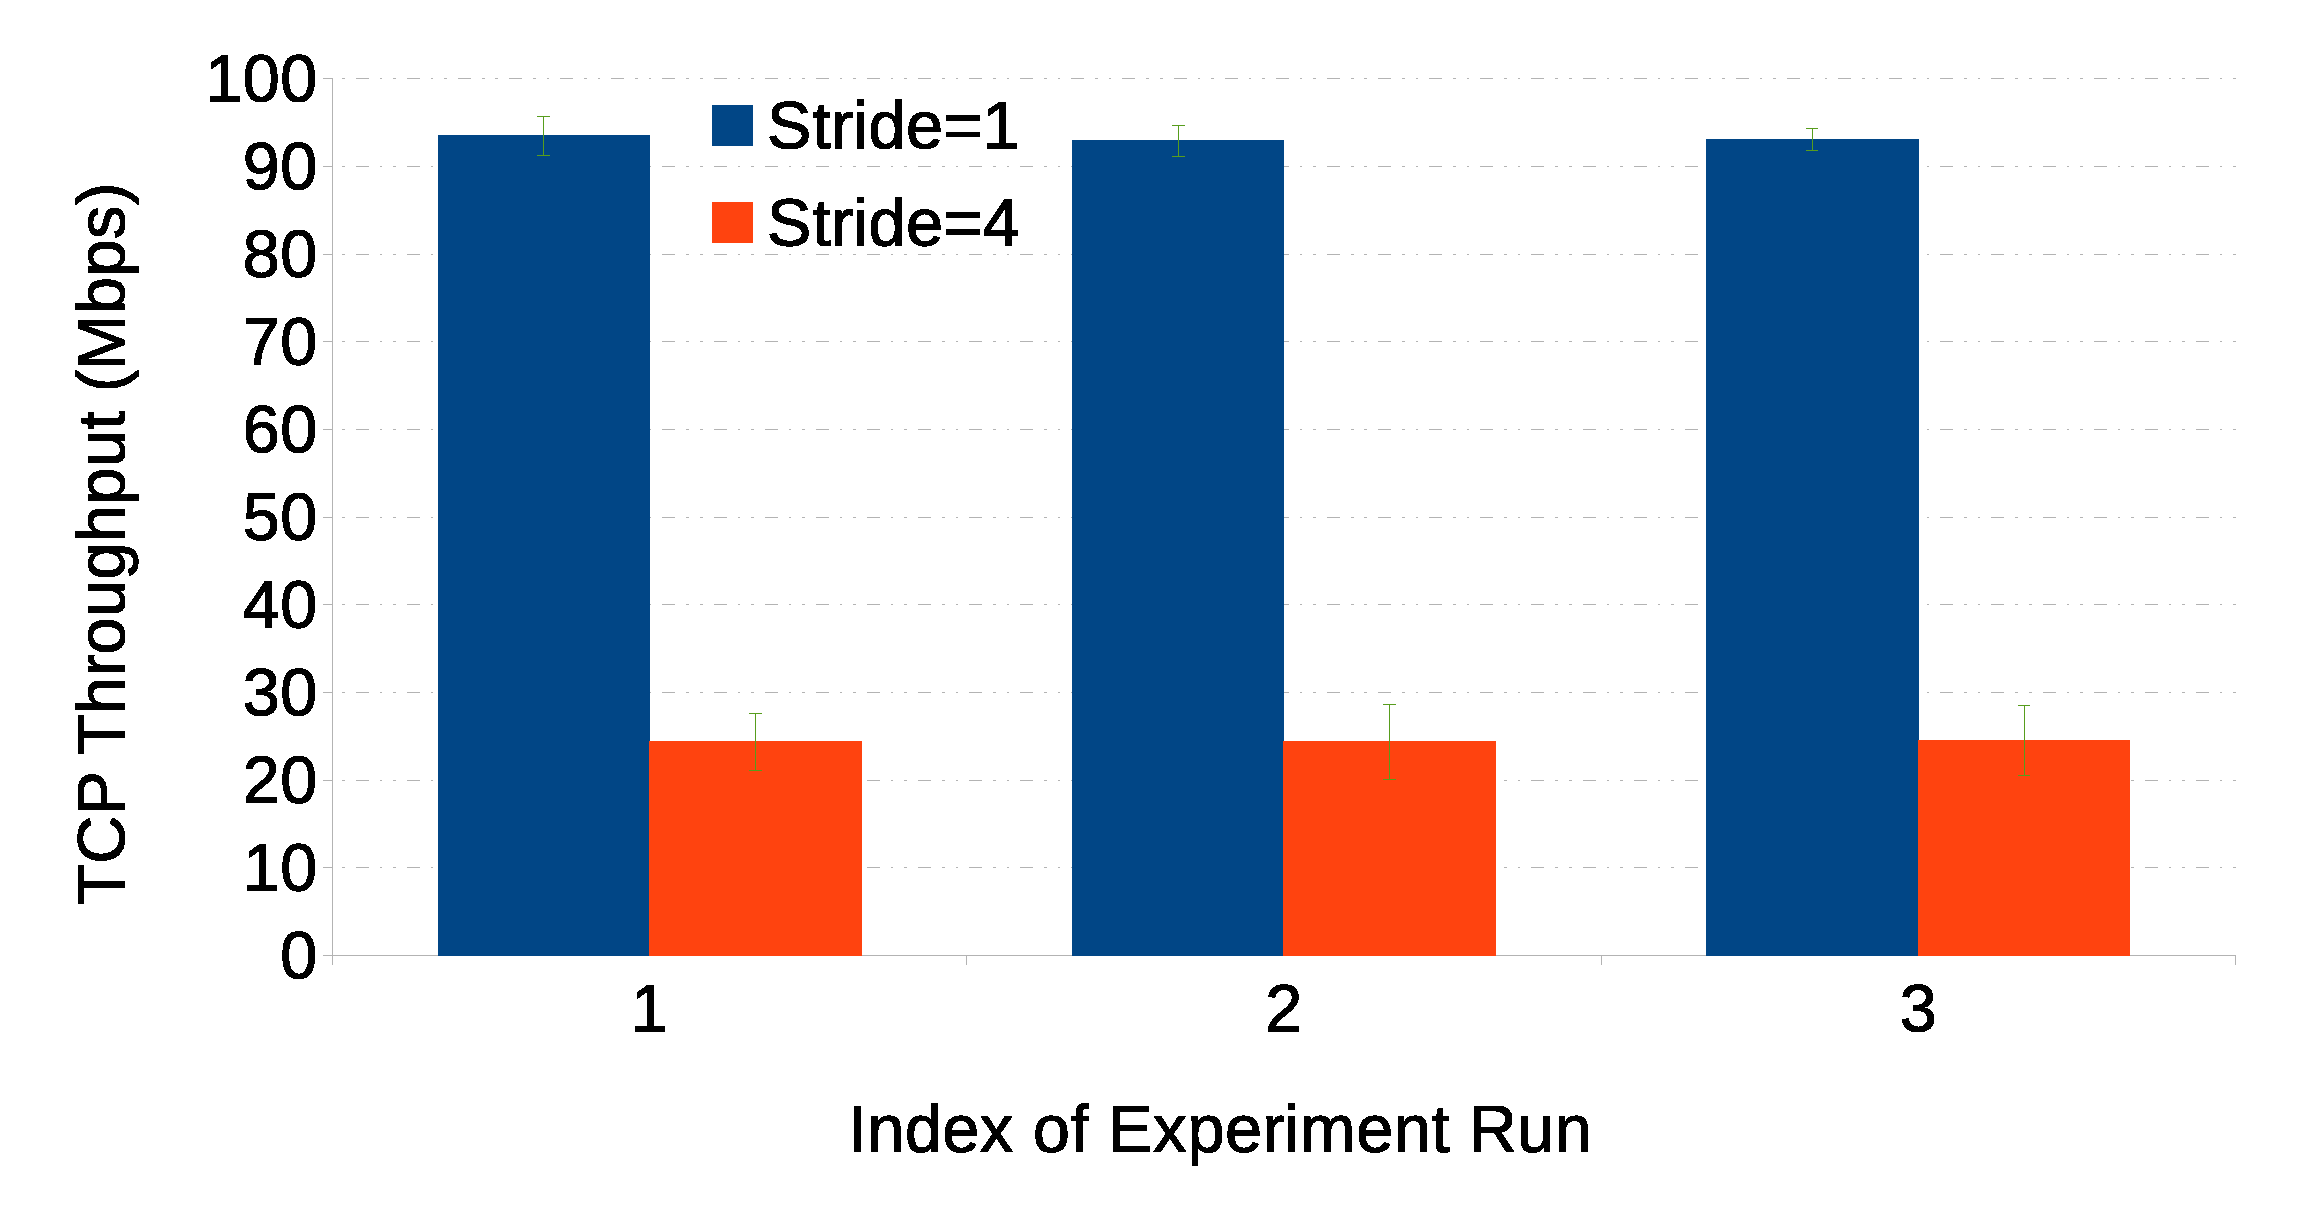
\epsfig{file=figures/FattreeAvgAggBw100M.eps, height=1.8in, width=3.5in}
		\label{Fig-FatTreeAvgBw100M}
	}~
	\subfloat[\textbf{Throughput of Individual TCP Flow}]{
		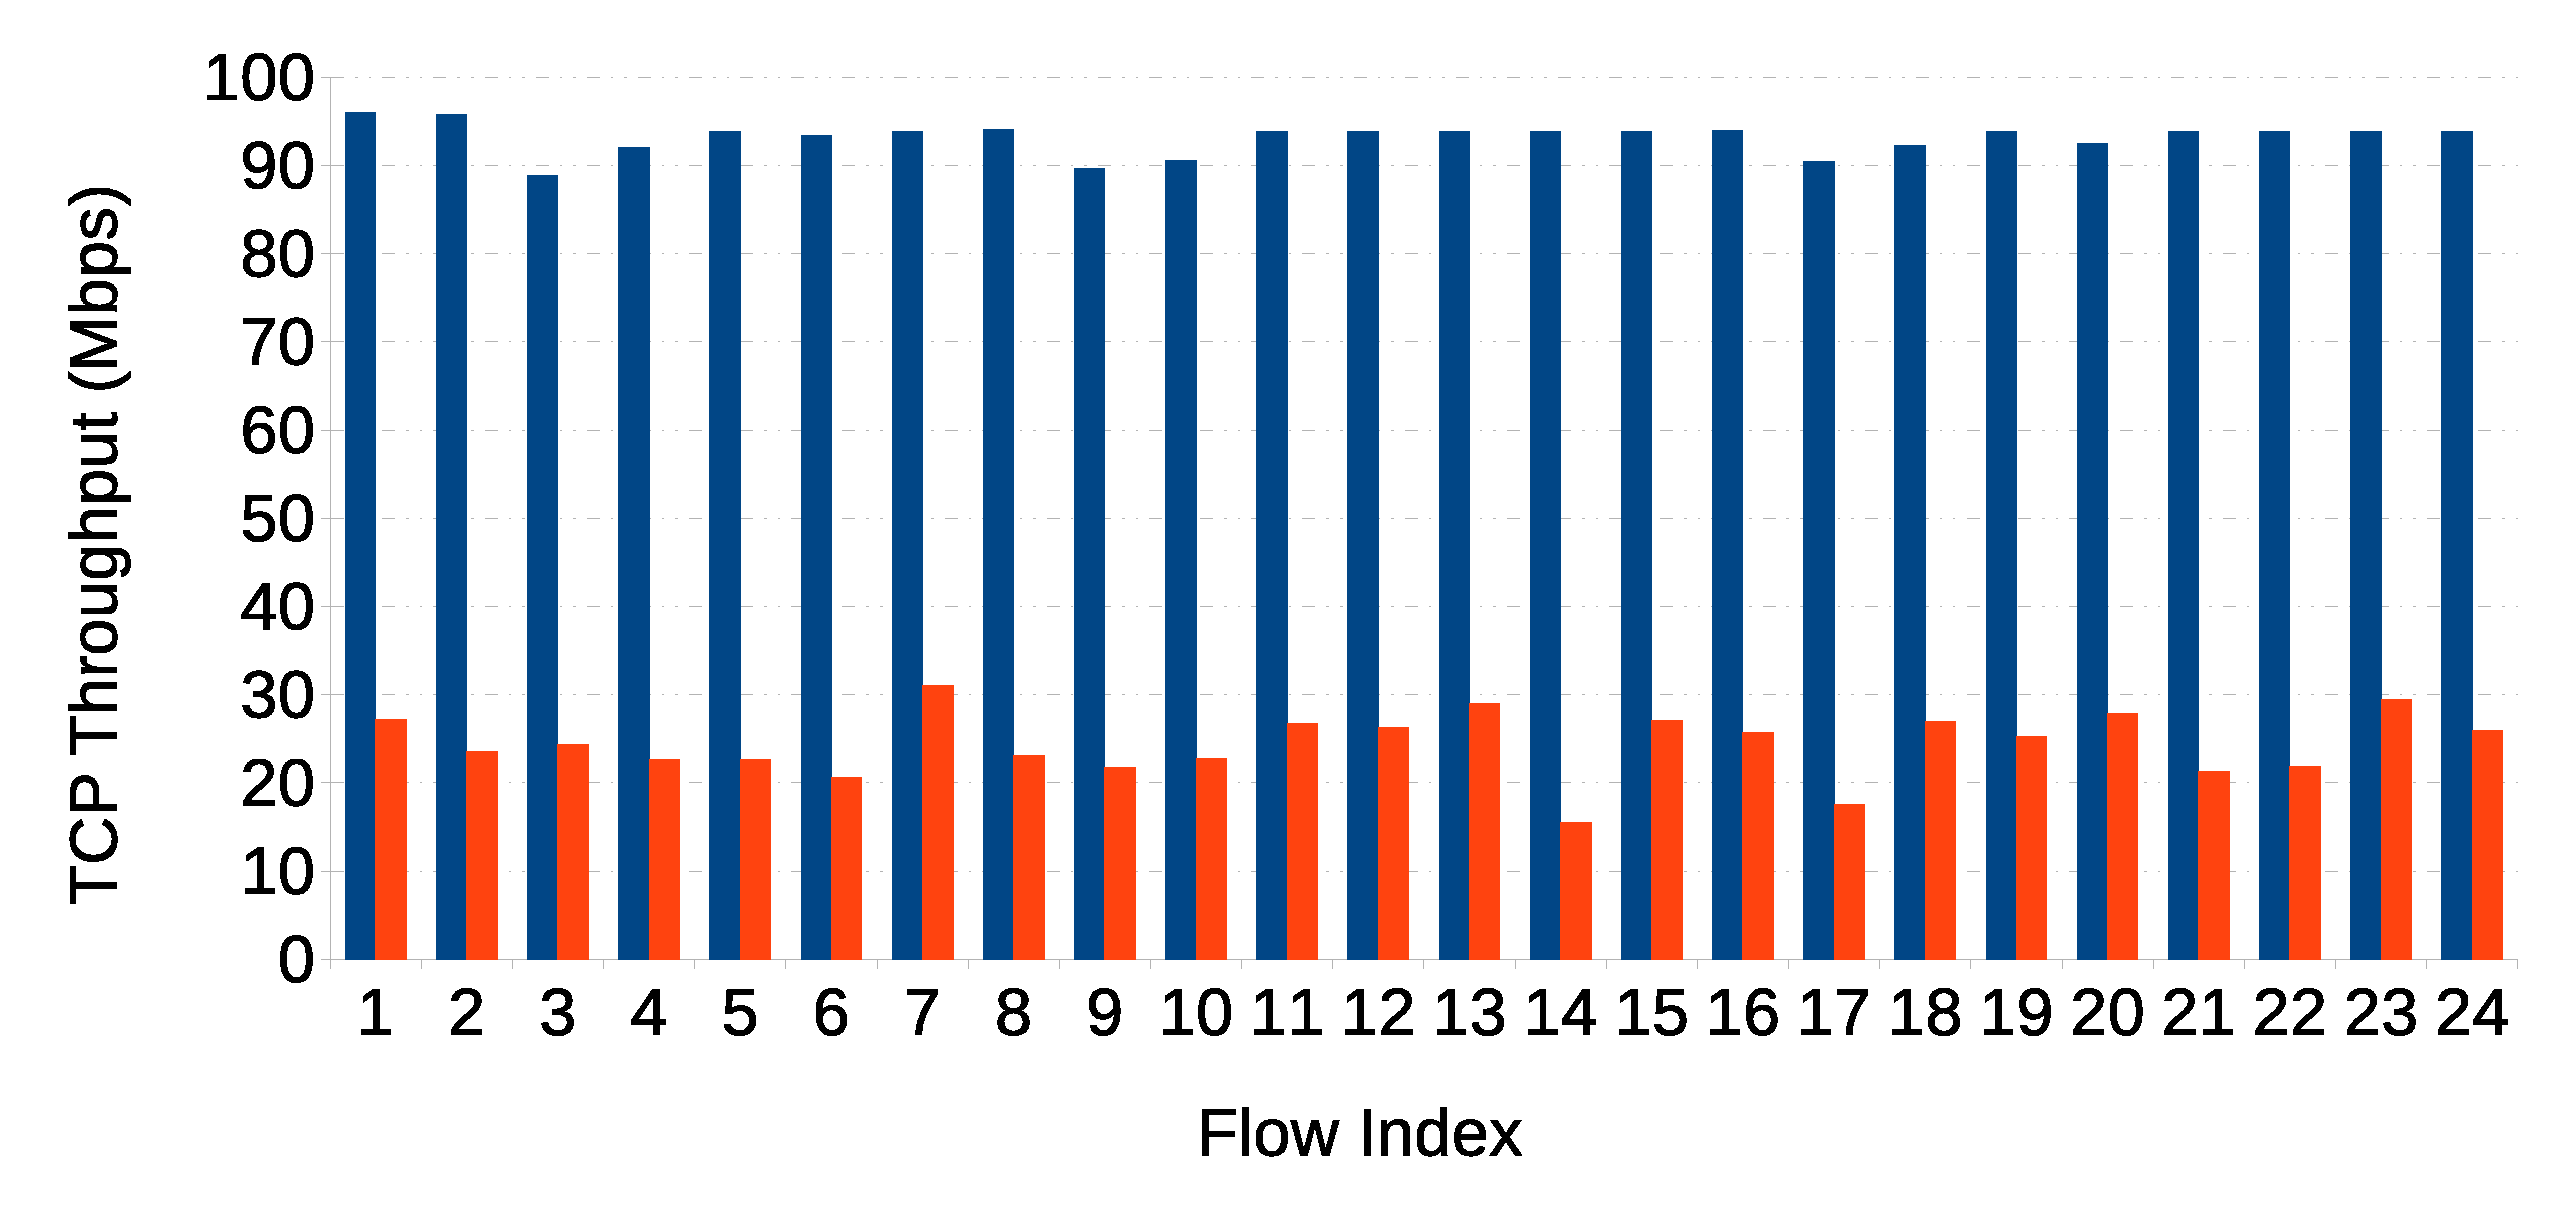
\epsfig{file=figures/FattreeFlowDistBw100M.eps, height=1.8in, width=3.5in}
		\label{Fig-FatTreeIndividualBw100M}
	}
\caption{\textbf{Mininet Emulation Results: ECMP Limitation in a Fat-tree-based Data Center Network with 100 Mbps Link Bandwidth}}
\end{figure*}

However, the link bandwidth configuration in the previous experiments are not realistic. As early as in 2009, links connecting edge hosts to top of rack switches (ToR), ToR to edge of rank switches (EoR), and EoR to Core switches in a data center had been already above gigabit, in particular, 10 Gbps switch-to-switch links and 1 Gbps host-to-switch links \cite{ScaleEffDCN}. Can Mininet still show us the limitation of ECMP with such high link bandwidth? If not, can virtual time help to overcome the issue? Using the same configurations except that links were set to 10 Gbps, we re-ran the experiments in Mininet without virtual time ($TDF=1$) and with virtual time ($TDF = 4$). We plotted the average flow throughput in Figure \ref{Fig-FatTreeAvgBw10G} and individual flow throughput in Figure \ref{Fig-FatTreeIndividualBw10G}.

\begin{figure*}[htbp]
\centering

	\subfloat[\textbf{Average TCP Flow Throughput}]{
		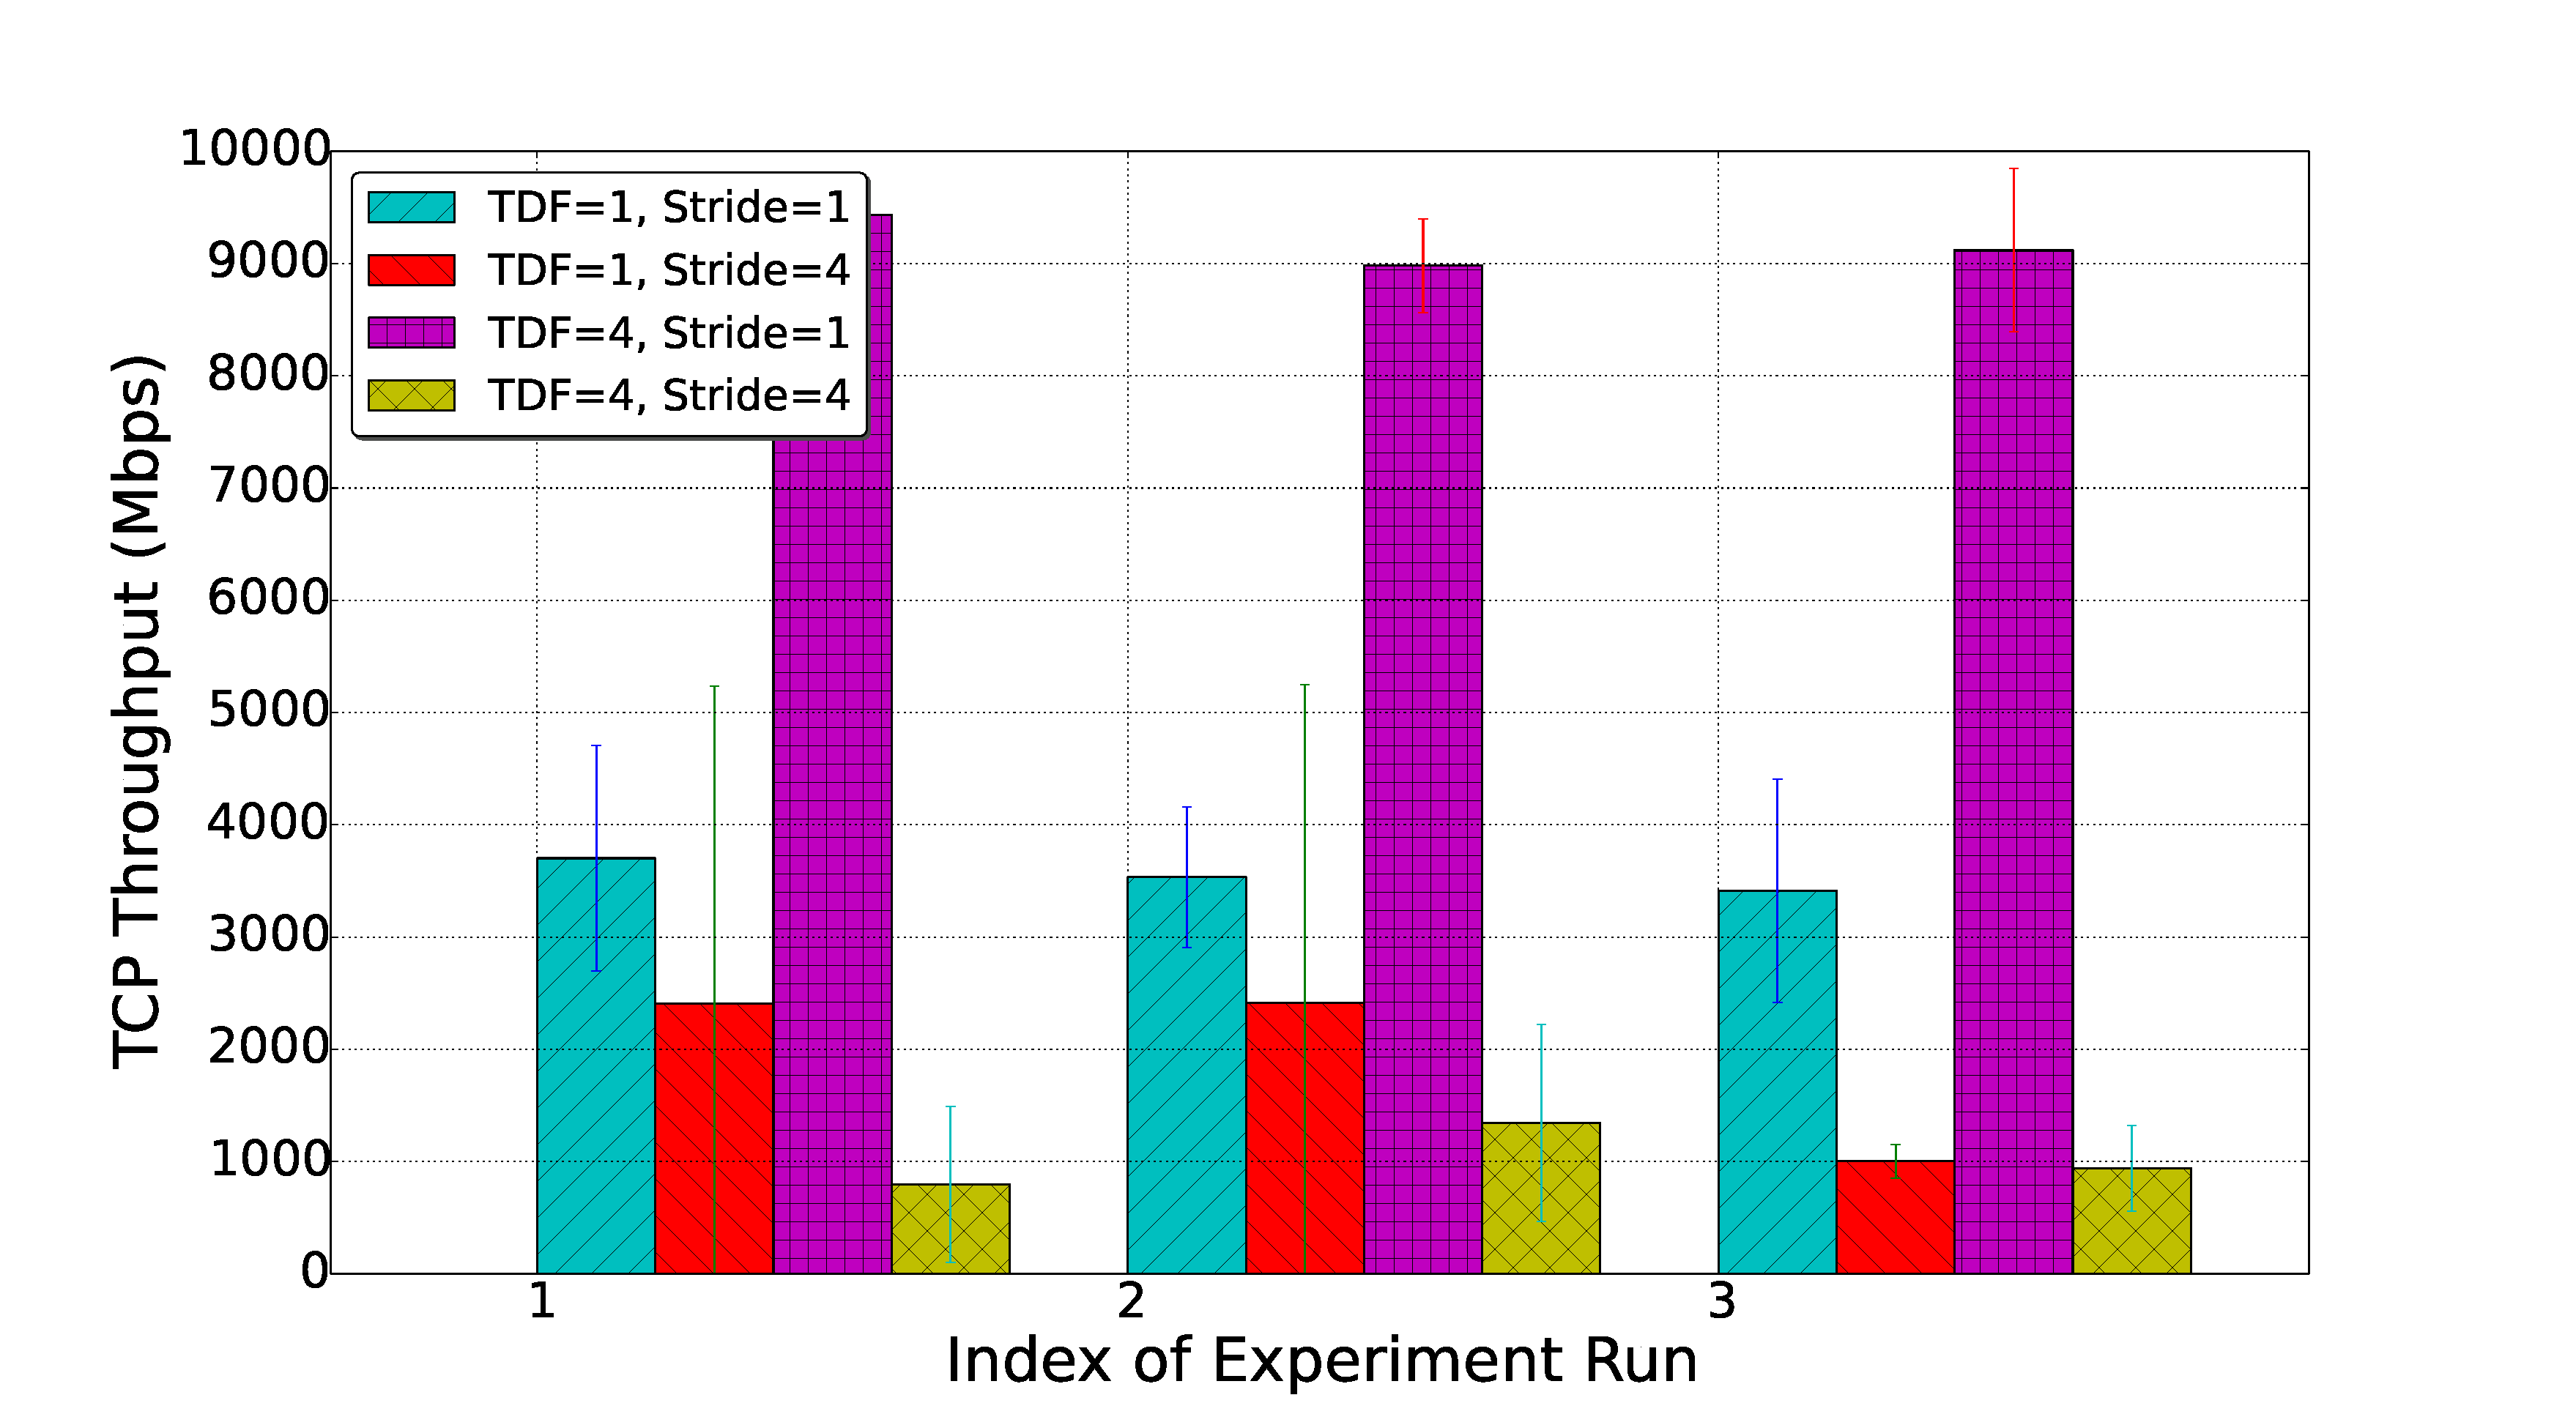
\epsfig{file=figures/FattreeAvgAggBw10G.eps, height=2.1in, width=3.5in}
		\label{Fig-FatTreeAvgBw10G}
	}~
	\subfloat[\textbf{Throughput of Individual TCP Flow}]{
		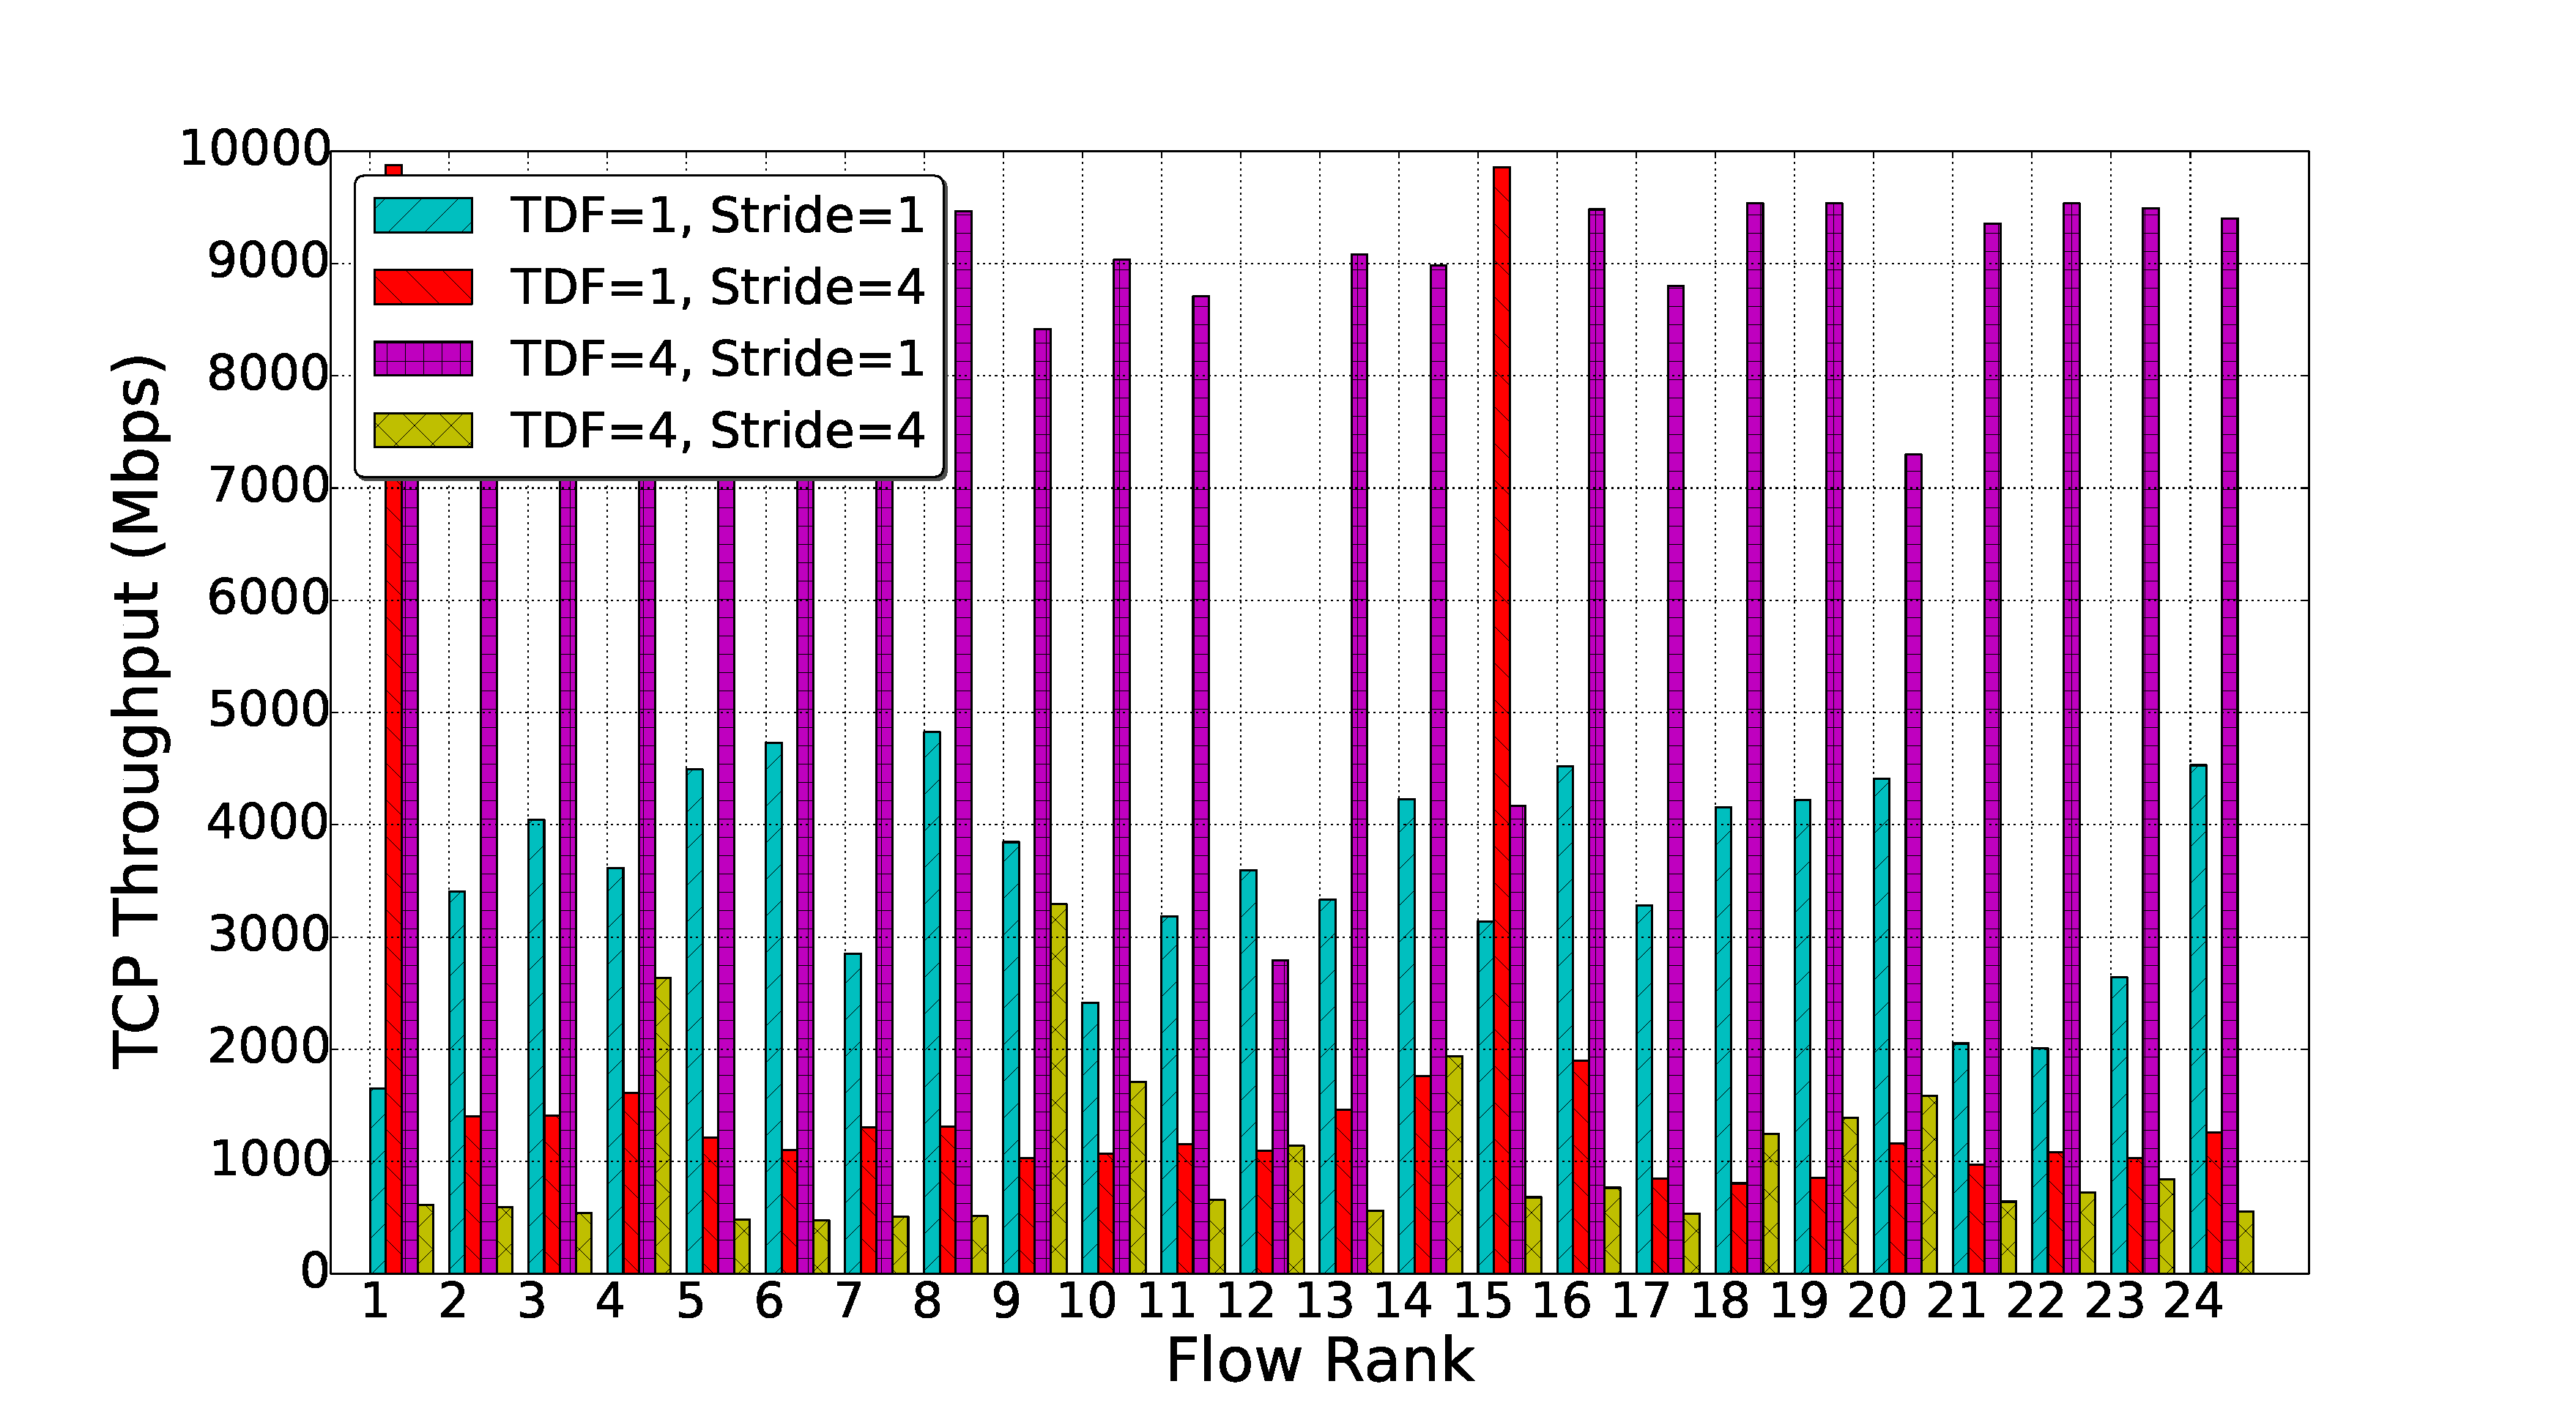
\epsfig{file=figures/FattreeFlowDistBw10G.eps, height=2.1in, width=3.5in}
		\label{Fig-FatTreeIndividualBw10G}
	}

%\caption{Demonstration of How Virtual Time Helps Find Limitation of ECMP in DCN with Fat Tree Topology: All link bandwidth are 10 Gbps}
\caption{\textbf{Mininet Emulation Results with Virtual Time: ECMP Limitation in a Fat-tree-based Data Center Network with 10 Gbps Link Bandwidth}}
\end{figure*}

\begin{table*}
\centering
\caption{\textbf{Lightweight Virtual Time System: Overhead of System Calls}}
\begin{tabular}{|c|c|c|c|c|} 
\hline
 & No Virtual Time & Virtual Time & Avg Overhead Per System Call \\%& Overhead Rate in E  \\ 
\hline
\texttt{gettimeofday}  & 0.0532 $\mu$s & 0.0661 $\mu$s & 0.0129 $\mu$s\\% & $3.0 \times 10^{-4}$\\ 
\hline
\texttt{settimedilationfactor} & 0  & 0.0628 $\mu$s & 0.0628 $\mu$s\\% & $3.65\times 10^{-9}$ \\ 
\hline
\end{tabular}
\label{Tab-Overhead}
\end{table*}


In the case of stride-1, there were very few collisions among flows. Hence, the network performance ought to be close to the ideal throughput, i.e., 160 Gbps bisection bandwidth and 10 Gbps average bandwidth between each pair. In the experiments that $TDF=4$, the average throughput is above 9.0 Gbps, which is close to the theoretical value, and also match well with the results obtained from the physical testbed built upon 37 machines \cite{Hedera}. In the experiments that $TDF=1$, however, the throughput barely reaches 3.8 Gbps because of the limited system resources that Mininet can utilize. In addition, as shown in Figure \ref{Fig-FatTreeIndividualBw10G}, we observe that the variation of throughput is large among flows when $TDF=1$. This is incorrect because no flow shares the same link in the case of stride-1. In contrast, when $TDF = 4$, the throughput of all 8 flows are close with little variation, which implies the desired networking behaviors. 

In the case of stride-4, flows may collide both on the upstream and the downstream paths, thus using ECMP could undergo a significant throughput drop, e.g., up to 61\% as experimentally evaluated in \cite{Hedera}.  The virtual-time-enabled Mininet ($TDF=4$) has successfully captured such throughput drop phenomenon. We can see that average throughput dropped about 80\% when RipL-Pox controller used ECMP to handle multi-path flows. Large deviation (more than 55\% of average throughput value) also indicates that the flows were not properly scheduled with ECMP. When $TDF=1$ (no virtual time), Mininet also reported plummeted TCP throughput in the case of stride-4. However, we cannot use the result to experimentally demonstrate the limitation of ECMP. It is hard to distinguish whether the throughput drop was caused by insufficient resources to handle 10 Gbps or the limitation of ECMP, given the fact that the throughput was already too low in the collision-free case. Without a correct baseline (benchmark for the collision-free scenario), it is difficult to perform further analysis and qualify the limitation.

% In the first place, Mininet-Hifi without virtual time cannot guarantee a good precondition: when nearly no flow collisions exist at first, the throughput performance of DCN is already abnormally low. On the other hand, even though we assume the reduced throughput when $stride =4$ is actually caused by ECMP, we cannot say too much about how serious it can be: without a correct baseline, it is impossible to estimate the percentage of throughput loss.  At last, one may argue that the reason of bandwidth loss in Mininet-Hifi without virtual time is mainly because the emulator is unable to handle too much intervening 10Gbps flows, instead of the flaw of the ECMP routing mechanism.



\section{Related Work}
\label{Sec-RelatedWorks}

\subsection{Virtual Time System}
Virtual time has been investigated to improve the scalability and fidelity of virtual-machine-based network emulation. 
There are two main approaches to develop virtual time systems. The first approach is based on time dilation, a technique to uniformly scale the virtual machine's perception of time by a specified factor. 
It was first introduced by Gupta et al. \cite{ToInfinityBeyond}, and has been adopted to various types of virtualization techniques and integrated with a handful of network emulators. 
Examples include DieCast\cite{DieCast}, SVEET\cite{SVEET}, NETbalance\cite{NETbalance}, TimeJails\cite{ComparisonVR-VM, TimeJails} and TimeKeeper\cite{TimeKeeper}. 
The second approach focuses on synchronized virtual time by modifying the hypervisor scheduling mechanism. 
Hybrid testing systems that integrate network emulation and simulation have adopted this approach. 
For example, \cite{jin2012virtual} integrates an OpenVZ-based virtual time system \cite{VirtTimeOpenVZ} with a parallel discrete-event network simulator by virtual timer.
SliceTime\cite{SliceTime} integrates ns-3\cite{NS-3} with Xen to build a scalable and accurate network testbed.

Our approach is technically closest to TimeKeeper \cite{TimeKeeper} through direct kernel modifications of time-related system calls. 
The differences are (1) we are the first to apply virtual time in the context of SDN emulation, (2) our system has a wider coverage of system calls interacting in virtual time, and (3) our system has an adaptive time dilation scheduler to balance speed and fidelity for emulation experiments.

\subsection{Adaptive Virtual Time Scheduling}
The key insight of virtual time is to trade time with system resources. 
Therefore, a primary drawback is the proportionally increased execution time. To determine an appropriate TDF, VENICE \cite{VirtualTimeMachine} proposes a static management scheme to forecast the recourse demand. 
One problem of static time dilation management is that we often assume the maximum load to ensure fidelity and thus overestimate the scaling factor. 

TimeJails \cite{TimeJails} presents a dynamic management scheme \cite{NtwkEmultAdaptVirtTime} to adjust TDF in run-time based on CPU utilization. 
We take a similar approach with two differences: the target platform and communication overhead. TimeJails is a Xen-based platform extended to a 64-node cluster for scalability, while our system supports more scalable experiments on a single machine with Linux container.
TimeJails requires a special protocol to prioritizing TDF request message in local area networks, while the communication overhead of our system is much lower, either through synchronized queues or method invocations among extended modules in the emulator.

% \newpage
\subsection{SDN Emulation and Simulation}
OpenFlow \cite{Openflow} is the first standard communications interface defined between the control and forwarding planes of an SDN architecture. 
Examples of OpenFlow-based SDN emulation testbeds include Mininet \cite{LaptopSDN}, Mininet-HiFi \cite{ReproNetExprCBE}, EstiNet \cite{EstiNet}, ns-3 \cite{NS-3} and S3FNet\cite{jin2013parallel}.
Mininet is currently the most popular SDN emulator, which uses process-based virtualization technique to provide a lightweight and inexpensive testbed. 
NS-3 \cite{NS-3} has an OpenFlow simulation model and also offers a realistic OpenFlow environment through its generic emulation capability, which has been linked with Mininet \cite{MininetLinkNS3}. 
S3FNet\cite{jin2013parallel} supports scalable simulation/emulation of OpenFlow-based SDN through a hybrid platform that integrates a parallel network simulator and a virtual-time-enabled OpenVZ-based network emulator \cite{S3F_website}. 
%Mininet support linking simulation with ns-3 \cite{MininetLinkNS3}.


% \subsection{Virtual Time}

% Nowadays, it is common to see emulators taking the advantage of virtualization technology like OpenVZ\cite{OpenVZ} or Xen\cite{Xen} to emulate large scale distributed system on single server or moderate cluster. After all, virtual machines now are easy to setup and control and have been always cost-efficient. Virtualization based emulator is also of high functional fidelity because in emulations real code are executed. However, it is limited by its limited physical resource when the scale of targeted distributed or network system increases. Hence, virtual time is widely used by many researchers to improve the scalability and efficiency of their emulators or testbeds.

% For example, Zheng and Nicol\cite{VirtTimeOpenVZ} have modified OpenVZ and OpenVZ's schedulers so as to measure the time used by virtual machine in computation and have Linux return virtual time to virtual machines. Lamps and Nicol\cite{TimeKeeper} design and implement a lightweight virtual time system TimeKeeper and integrated it with CORE\cite{CORE}. Our work bears similarity to that of the TimeKeeper, all take the advantage of Linux container mechanism. However, we want to use a simpler method to inject virtual time to Mininet's virtual hosts. 

% Many researchers\cite{ToInfinityBeyond, ComparisonVR-VM, SVEET, NETbalance} implemented virtual time on Xen virtual machines. Aside from implementation details, generally speaking, \textit{two} major modifications are needed to support time dilation in their emulation system. The first one goes to Xen's hypervisor (VM Monitor). It includes a shared data structure of wall clock time passing between Xen VMM and guesting OS and timer interrupts. Second, developers also need to modify guest OS's kernel to read appropriately scaled version of the hardware Time Stamp Counter (TSC). 

% \subsection{Adaptive Scheduling}

% The magic of virtual time, of course, comes with a cost. All the works mentioned above has two major problems. The first one is that it is subtle to select an adequate dilation value for entire experiment duration. A simple solution used by many emulators\cite{ToInfinityBeyond, SVEET, TimeJails} is to run the entire experiment with a enough large time dilation factor so that dilated resource matches that of the target system's. Sometimes this will lead to unacceptable running time. The second problem is that load generated by the experiment scenario may vary over time. Without a dynamic management scheme, one can only select  for the period with maximum load. When the experiment goes into a low load phase, emulator with fixed  cannot intelligently speed up the progress of the experiment.

% To solve the first problem, VENICE\cite{VirtualTimeMachine} has been adopted a two-level management scheme. At global level, they formulate the problem of finding appropriate time dilation factor as a optimal graph partition problem subjecting to resource constrains. At local level, they proposed load-driven and deadline-driven resource management solutions on VM scheduler, both depending on proper predictive method to forecasting resource needed with respect to future workload or progress deadline. Since time dilation factor can be determined when user setups emulation, we refer it as \textit{static virtual time management solution.}

% \cite{TimeJails} introduced the concept of Epochs to schedule time dilation factor. During an epoch, TDF remains constant and all physical nodes run under same TDF. At an epoch transition, all VMs synchronously switch to a new TDF. In an Epoch, a monitor collect information of emulation system load such as percentage of CPU time used by VMs and utilization of physical network. Whenever the emulator exceeds an overload or falls behind a underload warning threshold, a coordinator should initiate epoch transition and increase or decrease TDF. In their further works\cite{NtwkEmultAdaptVirtTime, NETapproach}, they implemented a simple but effective TDF adaptation scheme on the basis of the threshold of system load. We refer their work as \textit{dynamic virtual time management solution.}

\section{Conclusion and Future Works}
\label{Sec-Conclusion}
In conclusion, we present a Linux-container-based virtual time system and integrated it to a widely used SDN emulator, Mininet. The lightweight system uses a time-dilation-based design to offer virtual time to the containers, as well as the applications running inside the containers with no code modification. Experimental results show the promising fidelity and scalability improvement of Mininet with virtual time, particularly for high workload network scenarios. We have also used the platform to precisely evaluate the limitations of the ECMP routing in a realistic data center network with the results being validated by a physical testbed. Future works include the investigation of other effective control algorithms to further improve the adaptive TDF scheduler, and the integration to network simulators based on virtual time for large-scale network analysis.


% The following two commands are all you need in the
% initial runs of your .tex file to
% produce the bibliography for the citations in your paper.
\bibliographystyle{abbrv}
% \bibliography{sigproc}
% \clearpage
\bibliography{short}
% sigproc.bib is the name of the Bibliography in this case
% You must have a proper ".bib" file
%  and remember to run:
% latex bibtex latex latex
% to resolve all references
%
% ACM needs 'a single self-contained file'!
%
\end{document}
